\documentclass[a4paper]{article}
\usepackage[T1]{fontenc}			% \chapter package
\usepackage[english]{babel}
\usepackage[english]{isodate}  		% date format
\usepackage{graphicx}				% manage images
\usepackage{amsfonts}
\usepackage{booktabs}				% high quality tables
\usepackage{amsmath}				% math package
\usepackage{amssymb}				% another math package (e.g. \nexists)
\usepackage{bm}                     % bold math symbols
\usepackage{mathtools}				% emphasize equations
\usepackage{stmaryrd} 				% '\llbracket' and '\rrbracket'
\usepackage{amsthm}					% better theorems
\usepackage{enumitem}				% manage list
\usepackage{pifont}					% nice itemize
\usepackage{cancel}					% cancel math equations
\usepackage{caption}				% custom caption
\usepackage[]{mdframed}				% box text
\usepackage{multirow}				% more lines in a table
\usepackage{textcomp, gensymb}		% degree symbol
\usepackage[x11names]{xcolor}		% RGB color
\usepackage[many]{tcolorbox}		% colorful box
\usepackage{multicol}				% more rows in a table (used for the lists)
\usepackage{listings}
\usepackage{url}
\usepackage{qrcode}
\usepackage{fontawesome5}
\usepackage{ragged2e}
\usepackage{cite}                   % references
\usepackage{imakeidx}               % index
\makeindex[program=makeindex, columns=1,
           title=Index, 
           intoc,
           options={-s index-style.ist}]
\usepackage{fancyhdr}


\definecolor{codegreen}{rgb}{0,0.6,0}
\definecolor{codegray}{rgb}{0.5,0.5,0.5}
\definecolor{codepurple}{rgb}{0.58,0,0.82}
\definecolor{backcolour}{rgb}{0.95,0.95,0.92}
\lstdefinestyle{mystyle}{
    backgroundcolor=\color{backcolour},   
    commentstyle=\color{codegreen},
    keywordstyle=\color{magenta},
    numberstyle=\tiny\color{codegray},
    stringstyle=\color{codepurple},
    basicstyle=\ttfamily\footnotesize,
    breakatwhitespace=false,         
    breaklines=true,                 
    captionpos=b,                    
    keepspaces=true,                 
    numbers=left,                    
    numbersep=5pt,                  
    showspaces=false,                
    showstringspaces=false,
    showtabs=false,                  
    tabsize=2
}
\lstset{style=mystyle}


% draw a frame around given text
\newcommand{\framedtext}[1]{%
	\par%
	\noindent\fbox{%
		\parbox{\dimexpr\linewidth-2\fboxsep-2\fboxrule}{#1}%
	}%
}


% table of content links
\usepackage{xcolor}
\usepackage[linkcolor=black, citecolor=blue, urlcolor=cyan]{hyperref} % hypertexnames=false
\hypersetup{
	colorlinks=true
}


\newtheorem{theorem}{\textcolor{Red3}{\underline{Theorem}}}
\renewcommand{\qedsymbol}{QED}
\newcommand{\dquotes}[1]{``#1''}
\newcommand{\longline}{\noindent\rule{\textwidth}{0.4pt}}
\newcommand{\circledtext}[1]{\raisebox{.5pt}{\textcircled{\raisebox{-.9pt}{#1}}}}
\newcommand{\definition}[1]{\textcolor{Red3}{\textbf{#1}}\index{#1}}
\newcommand{\example}[1]{\textcolor{Green4}{\textbf{#1}}}
\newcommand{\highspace}{\vspace{1.2em}\noindent}


\begin{document}
    \newcounter{definition}[section]
    \newcounter{example}[section]
    
    \newtcolorbox[use counter = definition]{definitionbox}[1][]{%
        colback=red!5!white,
        colframe=red!75!black,
        fonttitle=\bfseries,
        title={Definition \thetcbcounter #1} %
    }
    
    \newtcolorbox[use counter = example]{examplebox}[1][]{%
        breakable,
        enhanced,
        colback=Green4!5!white,
        colframe=Green4!75!black,
        fonttitle=\bfseries,
        title={Example \thetcbcounter #1} %
    }

    %%%%%%%%%%%%%%%
    % Notes cover %
    %%%%%%%%%%%%%%%
    \author{260236}
\title{Software Engineering for HPC - Notes}
\date{\printdayoff\today}
\maketitle

    %%%%%%%%%%%
    % Preface %
    %%%%%%%%%%%
    \section*{Preface}

Every theory section in these notes has been taken from two sources:
\begin{itemize}
    \item None
\end{itemize}
About:
\begin{itemize}
    \item[\faIcon{github}] \href{https://github.com/PoliMI-HPC-E-notes-projects-AndreVale69/HPC-E-PoliMI-university-notes}{GitHub repository}
\end{itemize}
    
    %%%%%%%%%%%%%%%%%%%%%
    % Table of contents %
    %%%%%%%%%%%%%%%%%%%%%
	\tableofcontents
    \newpage

    %%%%%%%%%%%%%%%%%%%
    % Fancy pagestyle %
    %%%%%%%%%%%%%%%%%%%
    \pagestyle{fancy}
    \fancyhead{} % clear all header fields
    \fancyhead[R]{\nouppercase{\leftmark\hfill\rightmark}}

    %%%%%%%%%%%%%%%%
    % Introduction %
    %%%%%%%%%%%%%%%%
    \section{Software Configuration Management}

\subsection{Introduction}

\href{https://www.atlassian.com/microservices/microservices-architecture/configuration-management}{Configuration Management (CM)} is a systems engineering process for establishing consistency of a product's attributes throughout its life. In the technology world, configuration management is an IT management process that tracks individual configuration items of an IT system. IT systems are composed of IT assets that vary in granularity. An IT asset may represent a piece of software, or a server, or a cluster of servers. The following focuses on configuration management as it directly applies to IT software assets and software asset CI/CD.

\highspace
\definition{Software Configuration Management} is a \textbf{systems engineering process that tracks and monitors changes to a software systems configuration metadata}. In software development, configuration management is commonly used alongside version control and CI/CD infrastructure (explained later).

\highspace
The basic \textbf{approach to using a decentralized CM} is to have a repository (project) on the server side. 
\begin{itemize}
    \item When we want to work on the project, we clone the repository on the local PC. This workflow is used because we can work offline and on the local project without making critical changes to the repository server side.
    
    \item The local changes can be saved using the commit command and when we are ready to publish our changes, we use the push command to update the repository on the server side.
    
    \item After a push, anyone who has a local copy should make a pull command to update the local project.
\end{itemize}
This workflow can be done using git commands, and a good cheat sheet can be found \href{https://education.github.com/git-cheat-sheet-education.pdf}{here}.
    
    %%%%%%%%%%%%%%%%%%%%%%%%%%%%%%%%%%%%%%%%%%%%%%%%%%%%%%%%%%%%%%%%%%%
    % HPC Software, Relevant Qualities and System Engineering Methods %
    %%%%%%%%%%%%%%%%%%%%%%%%%%%%%%%%%%%%%%%%%%%%%%%%%%%%%%%%%%%%%%%%%%%
    \section{HPC Software, Relevant Qualities and Systems Engineering Methods}

\subsection{High Performance Computing Software}

There's no single definition of HPC, but it can be explained in a number of ways:
\begin{definitionbox}
    The practice of aggregating computing power in a way that delivers much high performance than one could get out of a typical desktop computer or workstation to solve large problems in science, engineering, or business.

    \highspace
    Thousands of processors working in parallel to analyze billions of pieces of data in real time, performing calculations thousands of times faster than a normal computer.

    \highspace
    The use of parallel processing for running advanced, large-scale application programs efficiently, reliably and very quickly on supercomputer systems.

    \highspace
    The platform technology concerned with programming for performance, where performance takes the broad meaning of:
    \begin{itemize}
        \item Speed (reducing time to solution);
        \item Energy efficiency (doing more with less power);
        \item Upscaling (handling larger problems such as simulating a wing aand then a full plane, or a cell and then an organ);
        \item High throughput (the ability to handle large volumes of data in near real-time, as required in the financial services industry, telecoms or satellite imagery).
    \end{itemize}
\end{definitionbox}

\noindent
As \definition{Parallel and Distributed Computing (PDC)} exist, it is necessary to explain the difference. The main characteristics of PDC are:
\begin{itemize}
    \item \textbf{Concurrency}: it is a property of software. \textbf{A piece of software is also concurrent if it can have more than one active execution context}.

    \item \textbf{Parallelism}: it is a property of software. \textbf{The execution of different tasks/pieces of software at the same time}.

    \item \textbf{Distribution}. \textbf{The execution of different tasks/pieces of software on physically distinct computing nodes connected through a network, lack of a global clock}.
\end{itemize}
\textbf{PDCs} are \textbf{multi-core machines}, whereas \textbf{HPCs} are \textbf{quantum computers}. However, \textbf{both share parallel machines}, \textbf{HPC clusters} and \textbf{cloud infrastructures}.

\newpage

\noindent
There are \textbf{two categories} of HPC software:
\begin{itemize}
    \item \definition{Compute-intensive applications}. These are \textbf{complex calculations that require a large number of computing resources}. They also often require parallel computing.

    \item \definition{Data-intensive applications}. They \textbf{focus on processing, storing and retrieving large amounts of data}. Typically built as distributed systems to ensure reliability and scalability.
\end{itemize}
    \subsection{Relevant Qualities}

For the two categories explained, there are some important characteristics:
\begin{itemize}
    \item For \definition{Compute-intensive applications}:
    \begin{itemize}
        \item \underline{\definition{Correctness}}: the \textbf{software is correct if it satisfies the specifications}, but be careful! Sometimes, modelling reality into a model (using the specifications) isn't the bigger problem. Instead, it is difficult or impossible to show actual correctness concerning reality. For \example{example}, imagine you are building a simulator of a planet lander before you have ever visited it.
        
        \emph{How can you fix this issue?} We can \textbf{check that the software output fulfils the important desired properties} and \textbf{identify and apply a measure of accuracy}.

        
        \item \underline{\definition{Performance}}: it is the \textbf{efficient use of resources}. Again, be careful! Is it a good idea? Is performance improvement always a good idea? Because it is \textbf{not necessarily if}:
        \begin{itemize}
            \item It makes software \textbf{more difficult to read} and \textbf{maintain}
            \item It \textbf{reduces the portability} of software
        \end{itemize}
        
        
        \item \underline{\definition{Portability}}.
        
        
        \item \underline{\definition{Maintainability}}. A system can have this feature if it follows \textbf{three principles}:
        \begin{enumerate}
            \item \definition{Operability}: \textbf{make it easy for the operations team to run the system and keep it running}. There are a number of things that need to be done to achieve this:
            \begin{itemize}
                \item Provide visibility into the runtime behavior and internals of the system, with good monitoring.

                \item Provide good support for automation and integration with standard tools.

                \item Avoidance of dependencies on individual machines (allowing machines to be taken down for maintenance while the system as a whole continues to run uninterrupted).

                \item Provide good documentation and an easy to understand operational model (\dquotes{If I do X, Y will happen}).

                \item Provide good default behavior, but also give administrators the freedom to override defaults when necessary.

                \item Self-healing when appropriate, but also giving administrators manual control over system state when needed.
            \end{itemize}
            
            \item \definition{Simplicity}: \textbf{make it easy for other software engineers to understand the system}. This is necessary because complex systems take more time to understand and increase the cost of maintenance. There are several techniques for doing this:
            \begin{itemize}
                \item Reducing \emph{accidental complexity}.
                
                \item Using abstractions, such as organising the architecture into well-defined components that hide the internal complexity behind a clear and easy-to-use interface; or reusing known solutions.
            \end{itemize}

            \item \definition{Evolvability}: make it easy for engineers to change the system as new requirements emerge. There are a number of things that need to be done to achieve this:
            \begin{itemize}
                \item Organize your development process to cope with evolution.
                
                \item Keep track of how requirements are mapped to your software structure.

                \item Update documentation.

                \item Continue to ensure simplicity and operability.
            \end{itemize}
        \end{enumerate}
    \end{itemize}

    \item For \definition{Data-intensive applications}:
    \begin{itemize}
        \item \underline{\definition{Reliability}}: can be mathematically defined as \textbf{probability of absence of failures for a certain period}. The typical expectations are:
        \begin{itemize}
            \item The application \textbf{performs the expected function}
            \item It can \textbf{tolerate mistakes by users}
            \item It \textbf{prevents unauthorized access} and \textbf{abuse}
        \end{itemize}
        
        
        \item \underline{\definition{Scalability}}: the \textbf{system ability to cope with increased load}. The load unit depends on the product: for web apps can be represented with the number of requests per second; for databases can be the number of read and write operation (or their ratio).
        
        
        \item \underline{\definition{Maintainability}}. Same as above.
    \end{itemize}
\end{itemize}
In the software, there can be some errors, but a software engineer should be able to recognize the type of failure, faults or defects:
\begin{itemize}
    \item A \definition{defect} is an \textbf{imperfection or deficiency in a work product} where that work product does \underline{not meet its requirements or specifications} and needs to be either repaired or replaced.

    \item A \textbf{defect encountered during software execution} is a \definition{fault} (a fault is a subtype of defect, and can be of two types, see below).
    
    \item A \definition{system failure} can be:
    \begin{itemize}
        \item Termination of the ability of a product to perform a required function or its inability to perform within previously specified limits.

        \item An event in which a system or system component does not perform a required function within specified limits.
    \end{itemize}
\end{itemize}
There are some exceptions where systems are \definition{fault-tolerant} or \definition{resilient}. These are systems that can \textbf{cope with faults and prevent faults from occurring}. An \textbf{advantage of fault-tolerance} is that \textbf{reliability is increased}. 

\newpage

\noindent
The \textbf{fault} can be of \textbf{two types}:
\begin{itemize}
    \item \definition{Hardware Faults}.
    \begin{flushleft}
        \textcolor{Red2}{\textbf{\faIcon{exclamation-triangle} Description of the problem}}
    \end{flushleft}
    It is a defect encountered during hardware execution. In a large datacenter these can happen on a daily basis. Different pieces of hardware usually fail independently from each other.
    \begin{flushleft}
        \textcolor{Green3}{\textbf{\faIcon{check} Possible solutions}}
    \end{flushleft}
    The possible solutions are two: \textbf{hardware redundancy} and \textbf{software fault-tolerance techniques}.

    \item \definition{Software Faults}.
    \begin{flushleft}
        \textcolor{Red2}{\textbf{\faIcon{exclamation-triangle} Description of the problem}}
    \end{flushleft}
    They result from \textbf{software development errors}. Can stay dormant for a long time and appear suddenly. They can \textbf{determine failures in multiple components} at the same time.
    \begin{flushleft}
        \textcolor{Green3}{\textbf{\faIcon{check} Possible solutions}}
    \end{flushleft}
    There is no single solution! It is a combination of strategies. So use defensive programming, by testing before release and during operation:
    \begin{itemize}
        \item Reboot the system frequently (rejuvenation)
        \item Continuous monitoring and alerting in case of possible symptoms
        \item Deliberately introduce failures to train the fault tolerance machinery (chaos engineering)
    \end{itemize}
\end{itemize}

\longline

\subsection{Systems Engineering Methods}

There are several systems engineering methodologies required in High Performance Computing:
\begin{itemize}
    \item Modelling the software structure and checking its properties.
    
    \item Performance analysis and improvement.
    
    \item Source code management.
    
    \item Documentation, standards, support to maintainability.
    
    \item Support to scalability.
    
    \item Attention to operability and automation.
\end{itemize}

    %%%%%%%%%%%%%%%%%%%%%%%%%%%
    % Requirement Engineering %
    %%%%%%%%%%%%%%%%%%%%%%%%%%%
    \section{Requirement Engineering}

\subsection{Definition}

Before the definition, we give a possible scenario to understand what requirement engineering is.

\highspace
The municipality of Milan says the following: \dquotes{\emph{The time it takes to make decisions on building permits for residential buildings in the city is too long. We want to develop software that will help us reduce this time}}. So where do we start? How do we identify the most important aspects? How do we make sure that we have understood what our customers want from us?

\begin{definitionbox}
    Software measure engineering (\definition{Requirement Engineering}) is the process of discovering the purpose for which the software is intended by identifying stakeholders and their needs, and documenting these in a form suitable for analysis, communication and subsequent implementation.
\end{definitionbox}

\noindent
The questions derived from requirements engineering are:
\begin{itemize}
    \item Identify stakeholders
    \item Identify their needs
    \item Produce documentation
    \item Analyze, communicate, implement requirements
\end{itemize}

\begin{figure}[!htp]
    \centering
    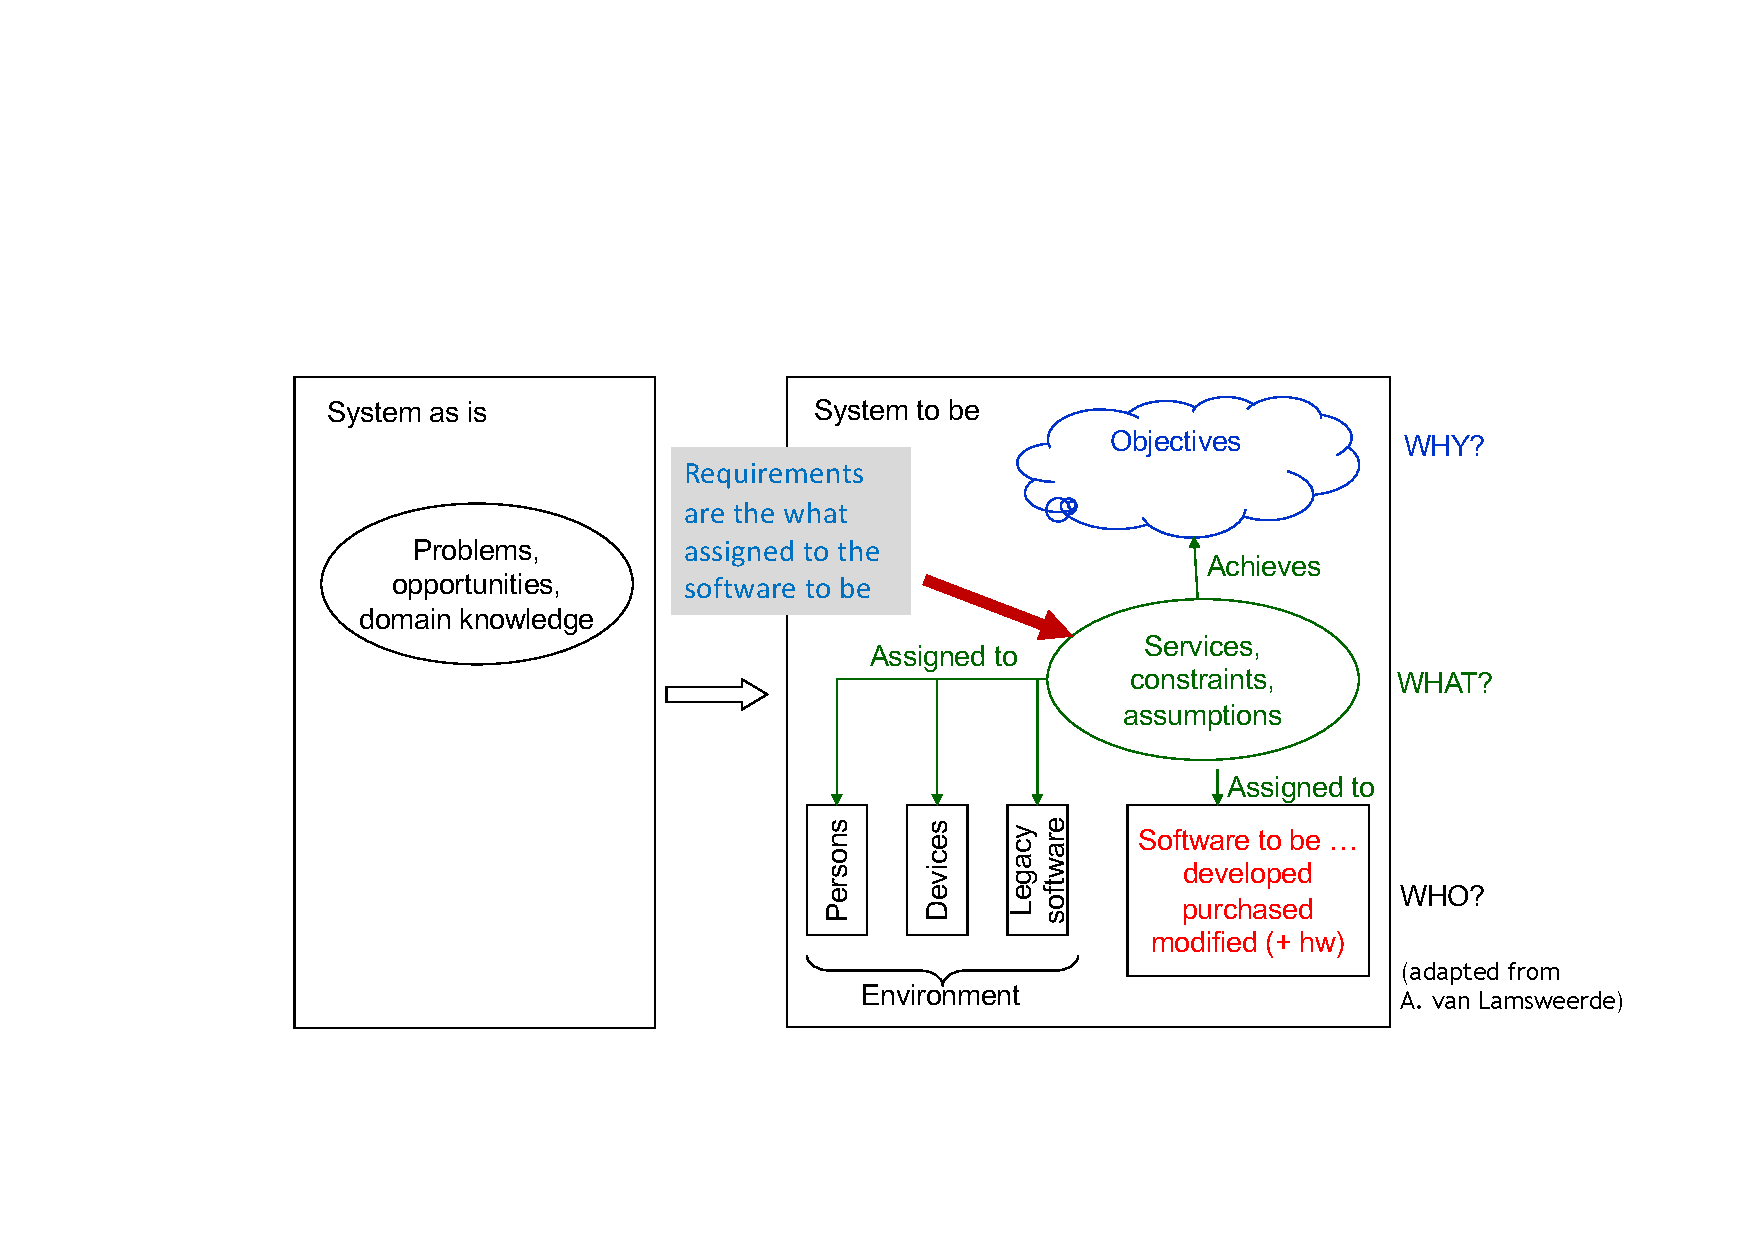
\includegraphics[width=\textwidth]{img/requirement-engineering-1.pdf}
    \caption{Analyzing the system as is and the system to be.}
\end{figure}
    \subsection{Studying the interplay between the world and the machine}

\begin{examplebox}[: ambulance dispatching system]\label{example: ambulance dispatching system}
    For every urgent call reporting an incident, an ambulance should arrive at the incident location within 14 minutes. For every urgent call, details about the incident are correctly encoded.

    When an ambulance is dispatched, it will reach the incident location in the shortest possible time. Accurate ambulance locations are known by GPS. Ambulance crews correctly notify ambulance availability through a mobile data terminal.

    \highspace
    Given the previous problem, are you able to extract requirements from this description? Some possible questions might be:
    \begin{itemize}
        \item Should the software system drive the ambulance?

        \item Who or what will \dquotes{correctly encode} details about incidents?
        
        \item Do terminals already exist or not?
    \end{itemize}
    And more in general:
    \begin{itemize}
        \item What are the boundaries of the system? What is inside/outside? What is in-between?

        \item How do we think about these aspects in a systematic way?
    \end{itemize}
\end{examplebox}

\noindent
This example is necessary to understand the \textbf{phenomena of world and machine}. The \definition{machine} \textbf{is the part of the system to be developed} (typically a software-to-be and a hardware). The \definition{world} (or environment) \textbf{is the part of the real world that is affected by the machine}.

\highspace
Requirements engineering is \textbf{concerned with the phenomena that occur in the world}. In the previous \example{example}, RE is concerned with the following phenomena:
\begin{itemize}
    \item Occurrence of incidents
    \item Reports of incidents by public calls
    \item Encoding of call details into dispatching software
    \item Assignment of an ambulance
    \item Arrival of an ambulance at the scene of an incident
\end{itemize}
But RE is also interested in the phenomena that occur inside the machine. In the previous \example{example}
\begin{itemize}
    \item The creation of a new object of the class \texttt{Incident}
    \item The updating of a database entry
\end{itemize}
\textbf{Requirements models are models of the world!}

\newpage

\noindent
Using the \example{example} on the previous page, we can show the phenomena we are interested in the world or in the machine set.
\begin{figure}[!htp]
    \centering
    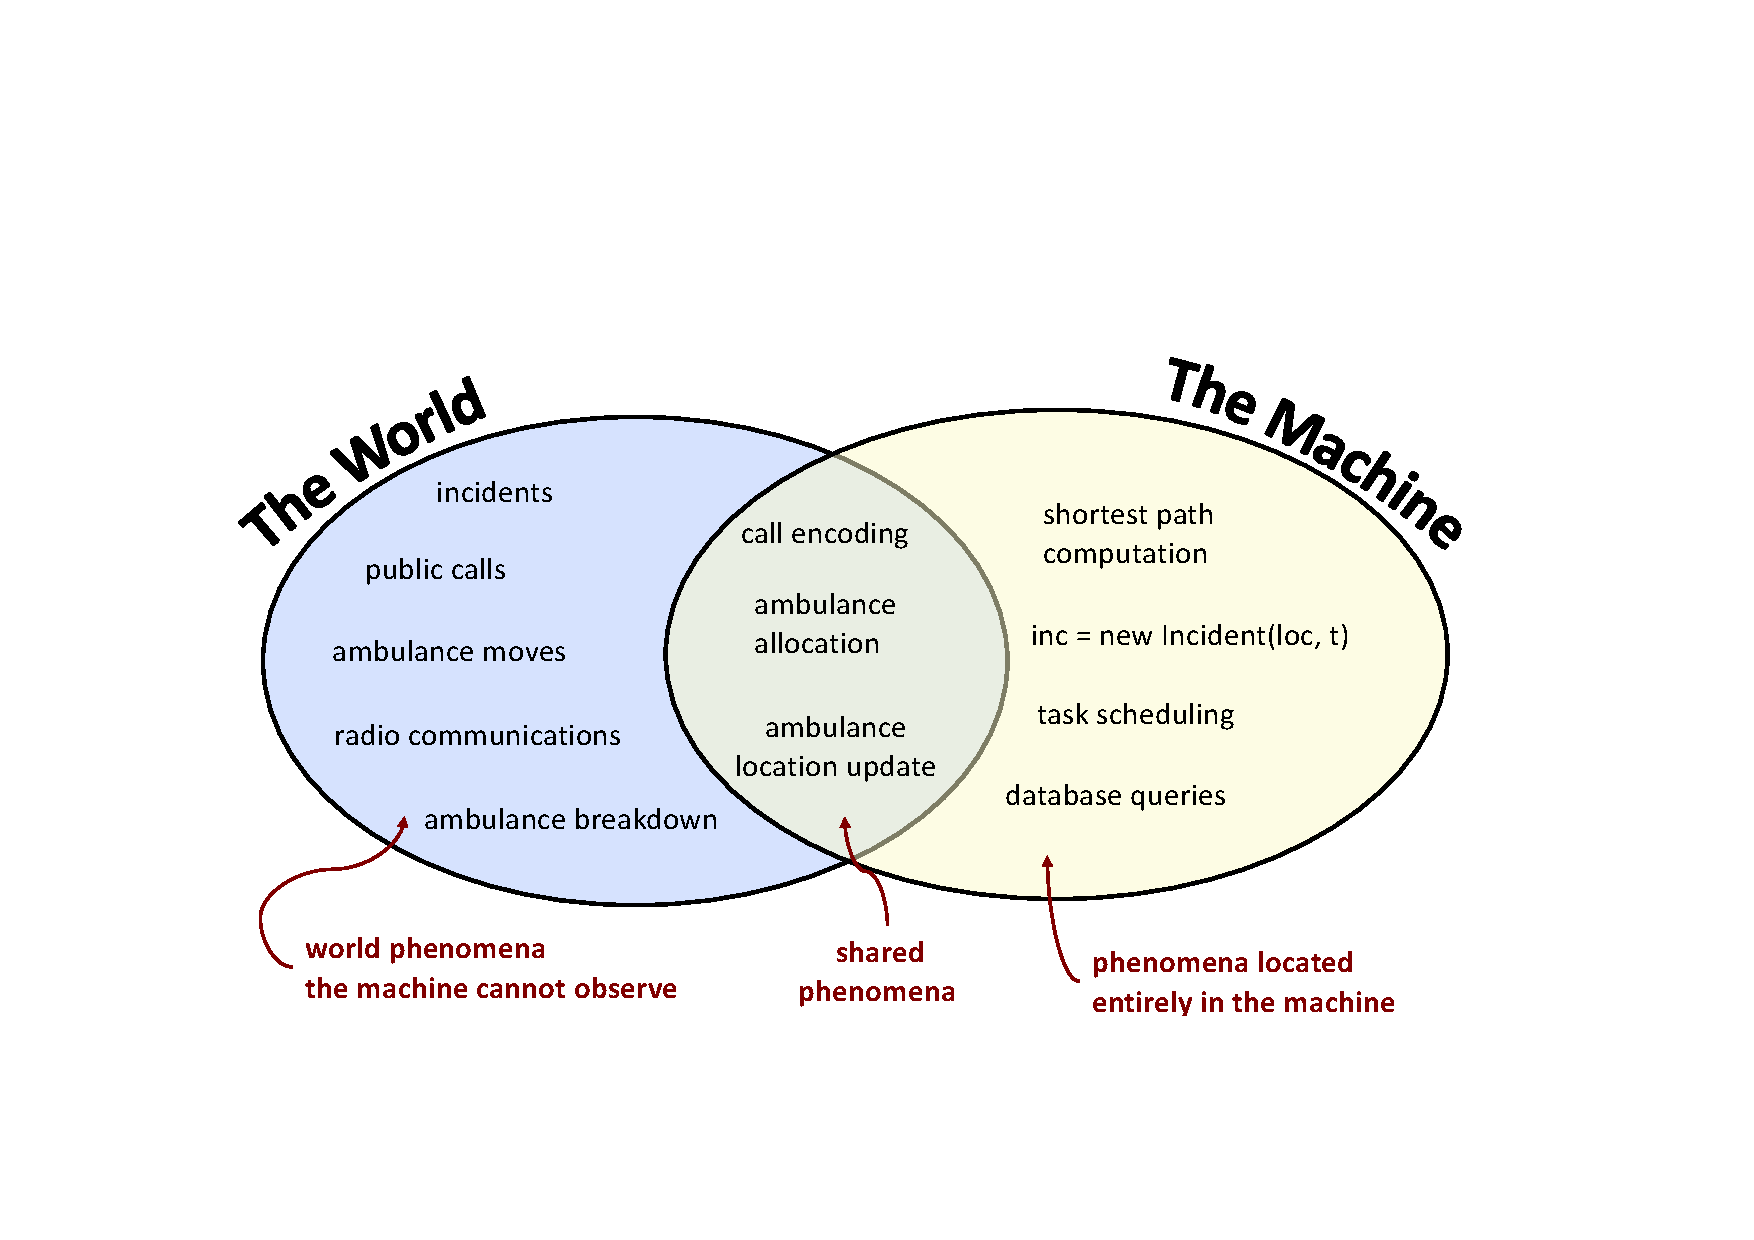
\includegraphics[width=\textwidth]{img/world-and-machine-1.pdf}
    \caption{The world and the machine sets, with reference to example on page~\pageref{example: ambulance dispatching system}.}
\end{figure}

\noindent
More generally, we can divide the machine and the world sets as:
\begin{itemize}
    \item The world which have goals and domain properties;
    \item The machine which have computers and programs;
    \item The requirements which is the bridge between the world and the machine.
\end{itemize}

\begin{figure}[!htp]
    \centering
    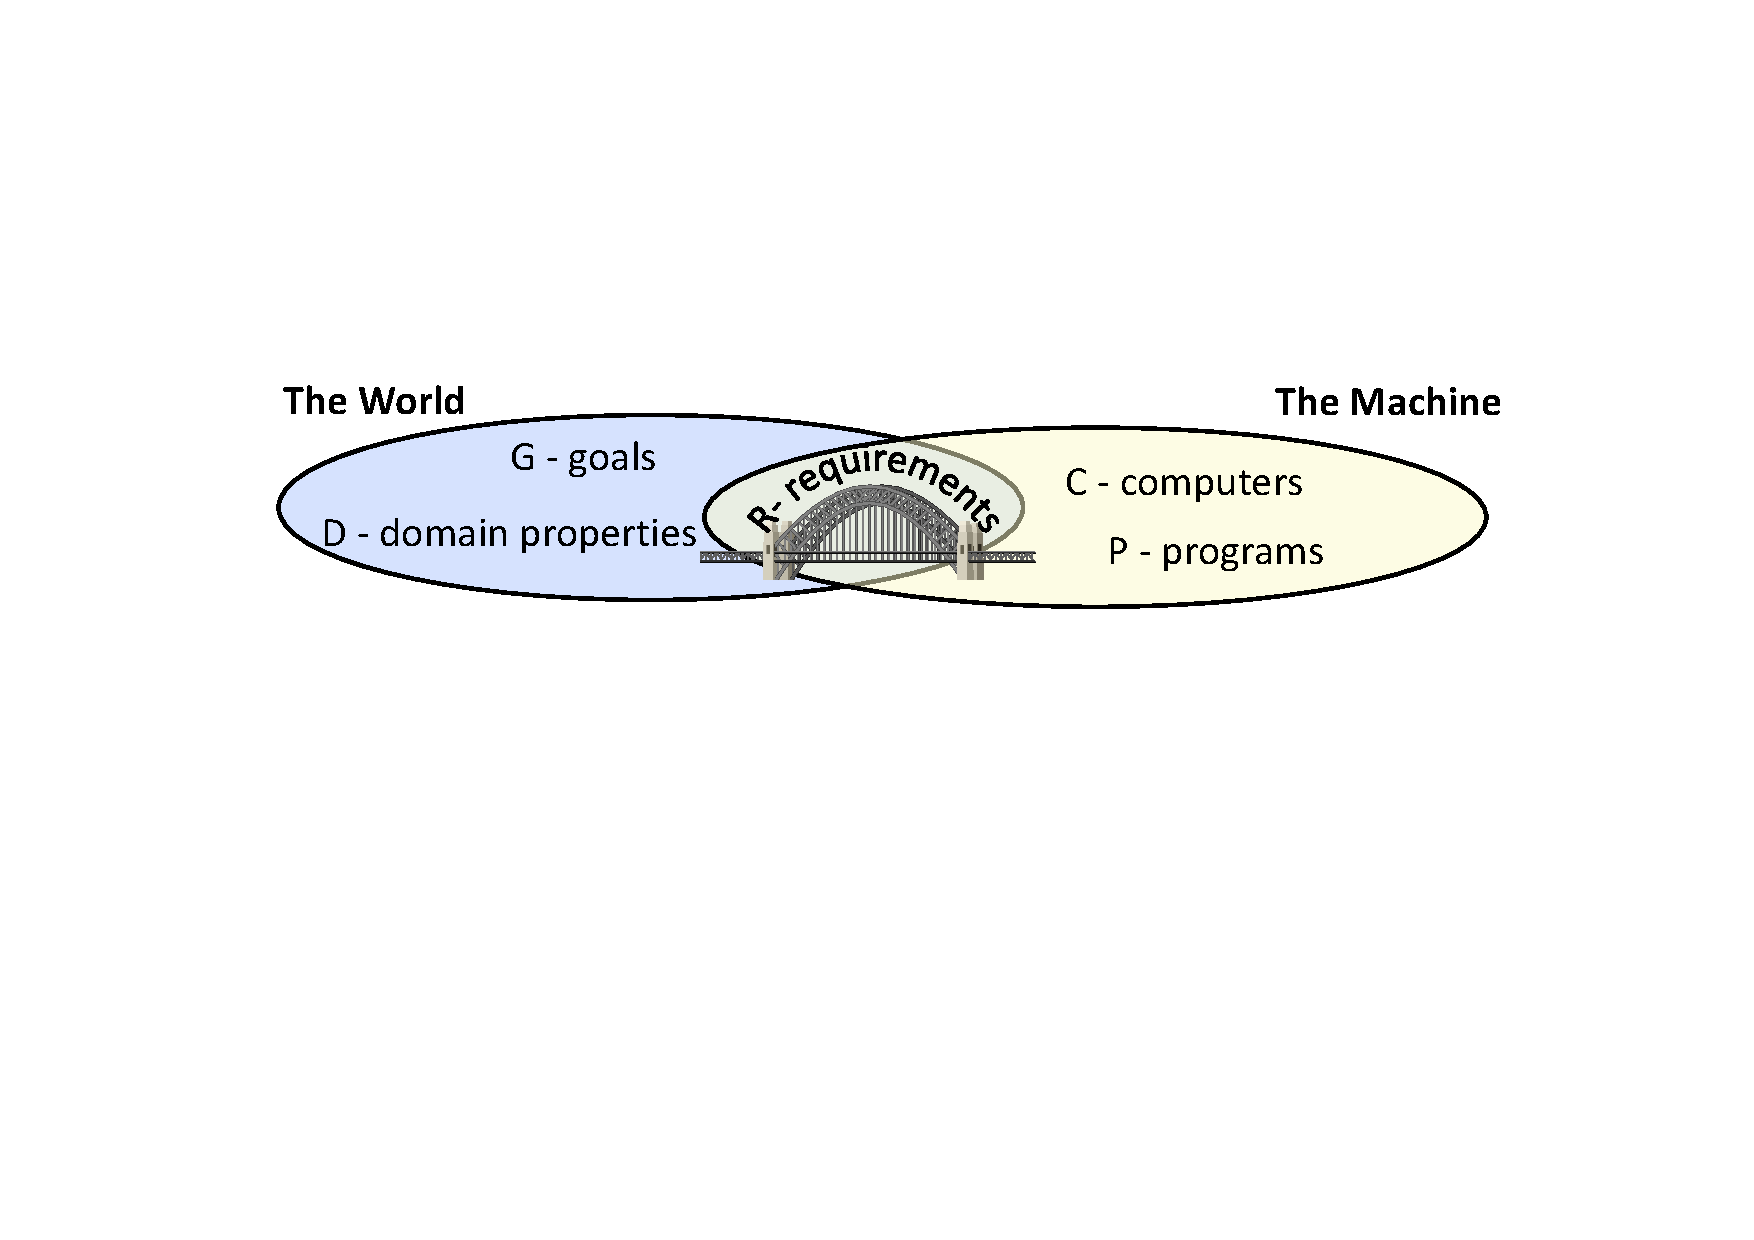
\includegraphics[width=\textwidth]{img/world-and-machine-2.pdf}
    \caption{Goals, domain properties, requirements, computers and programs.}
\end{figure}

\noindent
We explain more detailed these value inside the two sets:
\begin{itemize}
    \item \definition{Goals} are \textbf{prescriptive assertions formulated in terms of world phenomena} (not necessarily shared)
    \item \definition{Domain properties} (or assumptions) are \textbf{descriptive assertions assumed to hold in the world}
    \item \definition{Requirements} are \textbf{prescriptive assertions formulated in terms of shared phenomena} 
\end{itemize}

\newpage

\noindent
Using the \example{example} on the page~\pageref{example: ambulance dispatching system}, we can identify the goal, the domain assumptions and the requirement as follows:
\begin{itemize}
    \item \textbf{Goal}: \emph{For every urgent call reporting an incident, an ambulance should arrive at the incident scene within 14 minutes}.

    \item \textbf{Domain assumptions}:
    \begin{itemize}
        \item \emph{For every urgent call, details about the incident are correctly encoded}.
        \item \emph{When an ambulance is mobilized, it will reach the incident location in the shortest possible time}.
        \item \emph{Accurate ambulances' location are known by GPS}.
        \item \emph{Ambulance crews correctly signal ambulance availability through mobile data terminals on board of ambulances}.
    \end{itemize}
    
    \item \textbf{Requirement}: \emph{When a call reporting a new incident is encoded, the Automated Dispatching Software should mobilize the nearest available ambulance according to information available from the ambulances' GPS and mobile data terminals}.
\end{itemize}

\longline

\subsubsection{Completeness of Requirements}

Given the set of requirements \textbf{R}, goals \textbf{G} and domain assumptions \textbf{D}.

\begin{definitionbox}
    We say that \textbf{R} is \textbf{complete} \underline{if and only if}:
    \begin{itemize}
        \item \textbf{R} ensures satisfaction of \textbf{G} in the context of domain assumptions \textbf{D}
        \begin{center}
            \textbf{R and D $|=$ G}
        \end{center}
        We can make an analogy with program correctness. A program P running on a particular computer C is correct if it satisfies the requirement R: P and C $|=$ R.

        \item \textbf{G} captures all the \textbf{stakeholders' needs}.
        
        \item \textbf{D} represents \textbf{valid properties/assumptions about the world}.
    \end{itemize}
\end{definitionbox}
    \subsection{Formulating and classifying requirements}

The requirements can be of three types:
\begin{itemize}
    \item \definition{Functional requirements}: describe the interactions between the system and its environment (independent from implementation). In other words, are the \textbf{main} (functional) \textbf{goals the software has to realize}.
    
    For \emph{\example{example}}: \dquotes{\emph{the word processor shall allow users to search for strings in the text}}; \dquotes{\emph{the system shall allow users to reserve taxis}}.


    \item \definition{Non-functional requirements (NFRs)}: further characterization of user-visible aspects of the system not directly related to functions.
    
    For \emph{\example{example}}: \dquotes{\emph{the response time must be less than 1 second}}; \dquotes{\emph{the server must be available 24 hours a day}}.
    

    \item \definition{Constraints requirements}: imposed by the customer or the environment in which the system operates.
    
    For \emph{\example{example}}: \dquotes{\emph{the implementation language must be Java}}; \dquotes{\emph{the credit card payment system must be able to be dynamically invoked by other systems relying on it}}.
\end{itemize}
We make some observations about non-functional requirements. NFRs predicate on \textbf{external} non-functional qualities, and these qualities must be \textbf{measurable by metrics}. NFRs have some \underline{characteristics}:
\begin{itemize}
    \item Constraints on \textbf{how functionality must be provided to the end user}.

    \item The \textbf{application domain determines} their \textbf{relevance} and their \textbf{prioritization}.
    
    \item Have a \textbf{strong influence on the structure of the system to be built}. For \example{example}, a system may require 24/7 availability. As a result, it is likely to be designed as a replicated system (with redundant components).
\end{itemize}

\begin{examplebox}[: are these requirements?]
    \begin{enumerate}
        \item \dquotes{\emph{The user should insert correct information in the enrolment form}}.
    \end{enumerate}
    This is not a requirement! How can the software prevent a user from entering incorrect information? Specifically, is a domain assumption!

    \begin{enumerate}
        \setcounter{enumi}{1}
        \item \dquotes{\emph{The system should check whether fiscal code are well formed}}.
    \end{enumerate}
    Yes, the software can do this! So it is a requirement.
\end{examplebox}

\begin{examplebox}[: types of requirements]
    Example of \textbf{functional requirements}:
    \begin{itemize}
        \item \dquotes{\emph{The system shall allow users to reserve taxis}}.
        \item \dquotes{\emph{The system should never allowe non-registered users to see the list of other users willing to share a taxi}}.
        \item \dquotes{\emph{The system should guarantee that the reserved taxi picks the user up}}.
    \end{itemize}
    But attention! There is \textbf{unfeasible} (from the perspective of the software to be) \textbf{functional requirements}:
    \begin{itemize}
        \item \dquotes{\emph{The system should guarantee that the reserved taxi picks the user up}}.
    \end{itemize}
    This is because the software cannot guarantee this feature!

    \noindent
    Example of \textbf{non-functional requirements}:
    \begin{itemize}
        \item \dquotes{\emph{The system has to provide a feedback in 5 seconds}}.
        \item \dquotes{\emph{The system should be available 24/7}}.
    \end{itemize}
    Example of \textbf{technical requirements}:
    \begin{itemize}
        \item \dquotes{\emph{The system should be implemented in Java}}.
        \item \dquotes{\emph{The search for the available taxi should be implemented in class \texttt{Controller}}}.
    \end{itemize}
\end{examplebox}

\begin{examplebox}[: bad requirements]
    \begin{enumerate}
        \item \dquotes{\emph{The system shall process all mouse clicks very fast to ensure users do not have to wait}}.
    \end{enumerate}
    The problem here is that it \textbf{cannot be verified (tested)}, because what does \dquotes{fast} mean? Do we have a metric? Can you quantify it?

    \begin{enumerate}
        \setcounter{enumi}{1}
        \item \dquotes{\emph{The user must have Adobe Acrobat installed}}.
    \end{enumerate}
    The problem here is that it \textbf{cannot be achieved by the software system itself}. It is not something that the system has to do. \underline{But} it could be expressed as a domain assumption, so it is not a functional requirement for our software.
\end{examplebox}
    \subsection{Eliciting requirements}

The \definition{Requirements Elicitation} is the \textbf{practice of researching and discovering the requirements of a system from users, customers, and other stakeholders}. The \textbf{goal} of requirements elicitation is to ensure that the software development process is based on a clear and comprehensive understanding of the customer's needs and requirements. To do that, exist a simple and effective tool called \definition{scenario}s.

\begin{definitionbox}
    A \definition{scenario} is a concrete, focused, informal description of a single feature of the system to be.
\end{definitionbox}

\begin{examplebox}[: warehouse on fire]\label{example: warehouse on fire}
    \emph{Bob driving down main street in his patrol car notices smoke coming out of a warehouse. His partner, Alice, reports the emergency from her car.}

    \highspace
    \emph{Alice enters the address of the building, a brief description of its location (i.e. north west corner), and an emergency level. In addition to a fire unit, she requests several paramedic units on the scene given that area appears to be relatively busy. She confirms her input and waits for an acknowledgment.}

    \highspace
    \emph{John, the Dispatcher, is alerted to the emergency by a beep of his workstation. He reviews the information submitted by Alice and acknowledges the report. He allocates a fire unit and two paramedic units to the incident site and sends their estimated time of arrival (ETA) to Alice.}

    \highspace
    \emph{Alice received the acknowledgment and the ETA.}
\end{examplebox}
There are heuristics for finding scenarios, such as asking the customer a few questions:
\begin{itemize}
    \item Which user groups are supported by the system to perform their work?
    \item What are the primary tasks that the system needs to perform?
    \item What data will the actor create, store, change, remove or add in the system?
    \item What external changes does the system need to know about?
    \item What changes or events will the actor of the system need to be informed about?
\end{itemize}
However, it's very important \underline{not} \textbf{to rely on questionnaires alone}! \textbf{Insist on task observation} (if possible), ask to \textbf{speak to the end user}, not just the software contractor, and expect resistance, but try to overcome it.

\newpage

\noindent
Scenarios provide a nice summary of what the requirements analysis team can derive from observation, interviews, analysis of documentation. By generalizing the scenarios, we can get \definition{Use Cases}.

\highspace
To specify a use case, it's very important to follow the following scheme.
\begin{definitionbox}[: Use Cases Schema]
    \begin{itemize}
        \item \textbf{Name of Use Case}
        
        \item \textbf{Actors}
        \begin{itemize}
            \item \emph{Description of Actors involved in use case}.
        \end{itemize}
        
        \item \textbf{Entry condition}
        \begin{itemize}
            \item \dquotes{\emph{When this use case starts the following condition is true...}}.
        \end{itemize}
        
        \item \textbf{Flow of Events}
        \begin{itemize}
            \item \emph{Free form, informal natural language}.
        \end{itemize}
        
        \item \textbf{Exit condition}
        \begin{itemize}
            \item \dquotes{\emph{This use case terminates when the following condition holds...}}.
        \end{itemize}
        
        \item \textbf{Exceptions}
        \begin{itemize}
            \item \emph{Describe what happens if things go wrong}.
        \end{itemize}
        
        \item \textbf{Special Requirements}
        \begin{itemize}
            \item \emph{Nonfunctional Requirements, Constraints}.
        \end{itemize}
    \end{itemize}
\end{definitionbox}

\noindent
The following \textbf{suggestions} are useful in defining an appropriate use case:
\begin{itemize}
    \item Use cases named with verbs that indicate what the user is trying to accomplish
    \item Actors named with nouns
    \item Use cases steps in active voice
    \item The causal relationship between steps should be clear
    \item A use case per user transaction
    \item Separate description of exceptions
    \item Keep use cases small (no more than two/three pages)
    \item The steps accomplished by actors and those accomplished by the system should be clearly distinguished (this helps us in identifying the boundaries of the system)
\end{itemize}

\newpage

\noindent
First of all, we present an example of a \textbf{bad use case}.
\begin{examplebox}[: bad use case]
    \example{Example} of a bad use case referring to the ambulance dispatching example on page~\pageref{example: ambulance dispatching system}:
    \begin{itemize}
        \item Use case name: Accident
        \item Participating Actors:
        \begin{itemize}
            \item Field Officer
        \end{itemize}
        \item Flow of Events:
        \begin{enumerate}
            \item The Field Officer reports the accident
            \item An ambulance is dispatched
            \item The Dispatcher is notified when the ambulance arrives on site
        \end{enumerate}
    \end{itemize}
    The \underline{errors} are as follows:
    \begin{itemize}
        \item In the \emph{use case name} field, the \textbf{word is a noun}. It's better to use a verb that indicates what the user is trying to achieve.
        
        \item The Dispatcher actor is \textbf{not declared} in the \emph{Participating Actors} field, but is mentioned in the \emph{Flow of Events} field.

        \item There are two main errors in the \emph{Flow of Events} section: the first is in the sentence \dquotes{\emph{An ambulance is dispatched}}. But \textbf{who sends it?} The second is in the third sentence, because \textbf{who notifies the Dispatcher?}
    \end{itemize}
\end{examplebox}

\noindent
Now we present an example of a \emph{well composed} use case.
\begin{examplebox}[: use case \texttt{ReportEmergency} with reference to the example on page~\pageref{example: warehouse on fire}]
    There are two \textbf{actors} involved:
    \begin{itemize}
        \item Field Officer (Bob and Alice in the Scenario)
        \item Dispatcher (John in the Scenario)
    \end{itemize}
    The \textbf{Entry Condition} is always true because an emergency can be reported at any time. The \textbf{sequence of events} is as follows:
    \begin{itemize}
        \item The \textbf{FieldOfficer} activates the Report Emergency function of her terminal.

        \item \textbf{Friend} (the system to be developed) responds by presenting a form to the officer.
        
        \item The FieldOfficer fills the form, by selecting the emergency level, type, location, and brief description of the situation. The FieldOfficer also describes possible responses to the emergency situation. Once the form is completed, the FieldOfficer submits the form.
        
        \item At which point, the \textbf{Dispatcher} is notified.
        
        \item The Dispatcher reviews the submitted information and allocates resources by invoking the AllocateResources use case. The Dispatcher selects a response and acknowledges the emergency report.
    \end{itemize}
    The \textbf{Exit Condition} is the following: the FieldOfficer has received the acknowledgment and the selected response.

    \highspace
    There are two possible \textbf{exceptions}:
    \begin{itemize}
        \item The FieldOfficer is notified immediately if the connection between her terminal and the control room is lost.
        \item The Dispatcher is notified immediately if the connection between any logged in FieldOfficer and the control room is lost.
    \end{itemize}
    And the \textbf{special requirements} are:
    \begin{itemize}
        \item The FieldOfficer's report is acknowledged within 30 seconds;
        \item The selected response arrives no later than 30 seconds after it is sent by the Dispatcher.
    \end{itemize}
\end{examplebox}

\begin{examplebox}[: use case \texttt{AllocateResources} with reference to the example on page~\pageref{example: warehouse on fire}]
    \begin{itemize}
        \item Use case name: AllocateResources
        \item Participating Actors:
        \begin{itemize}
            \item Dispatcher (John in the Scenario. The Dispatcher allocates a resources to an Emergency if the resource is available; of course, he also updates and removes Emergency Incidents, Actions, and Requests in the system)
            
            \item Resource Allocator (the Resource Allocator is responsible for allocating resources in case they are scarce)
            
            \item Resources (the Resources that are allocated to the Emergency)
        \end{itemize}
        \item Entry Condition:
        \begin{itemize}
            \item An Incident has been opened
        \end{itemize}
        \item Flow of Events:
        \begin{itemize}
            \item The Dispatcher selects the types and number of Resources that are needed for the incident.
            
            \item Friend replies with a list of Resources that fulfill the Dispatcher's request.
            
            \item The Dispatcher selects the Resources from the list and allocates them for the incident.
            
            \item Friend automatically notifies the Resources.

            \item The Resources send a confirmation.
        \end{itemize}
        \item Exit Condition:
        \begin{itemize}
            \item The use case terminates when the resource is committed.
            \item The selected Resource is now unavailable to any other Emergences or Resource Requests.
        \end{itemize}
        \item Exceptions:
        \begin{itemize}
            \item If the list of Resources provided by Friend is insufficient to fulfill the needs of the emergency, the Dispatcher informs the Resource Allocator.
            \item The Resource Allocator analyzes the situation and selects new Resources by decommitting them from their previous work.
            \item Friend automatically notifies the Resources and the Dispatcher.
            \item The Resources send a confirmation.
        \end{itemize}
    \end{itemize}
\end{examplebox}

    %%%%%%%%%%%%%%%%%%%
    % Software Design %
    %%%%%%%%%%%%%%%%%%%
    \section{Software Design}

\subsection{Software Architecture}

\begin{definitionbox}
    The \definition{Software Architecture (SA)} of a system is the \textbf{set of structures} needed to reason about the system. These structures comprise software \textbf{elements}, \textbf{relations} among them, and \textbf{properties} of both.
\end{definitionbox}

\noindent
The software architecture is a tool for thinking about systems, and it's made up of a set of structures.

\highspace
The Architecture is so important because it is the vehicle for communication: internal (different teams) and external (teams and stakeholders). The Architecture manifests the first set of design decisions and is a portable abstraction of a system.
    \subsection{Architecture and multiple structures}

There is a set of structures relevant to the software:
\begin{itemize}
    \item \definition{Component-and-connector (C\&C)} structures. Describe how the system is structured as a \textbf{set of elements} that have \textbf{runtime behavior} (called components) and interactions (called connectors).
    \begin{itemize}
        \item The \textbf{components} are the principal units of computation (for \example{example} the clients, servers, services, etc.)

        \item The \textbf{connectors} represent communication (for \example{example} request-response mechanisms, pipes, asynchronous messages, etc.)
    \end{itemize}
    The \emph{\textbf{\underline{purpose}}} of these structures is to \textbf{enable us to answer questions} such as:
    \begin{itemize}
        \item \emph{What are the major executing components and how do they interact at runtime?}

        \item \emph{What are the major shared data stores?}
        
        \item \emph{Which parts of the system are replicated?}

        \item \emph{How does data progress through the system?}

        \item \emph{Which parts of the system can run in parallel?}

        \item \emph{How does the system's structure evolve during execution?}
    \end{itemize}
    Also, \textbf{allow us to study runtime properties} such as availability and performance.

    \item \definition{Module} structures. Show how a system is structured as \textbf{a set of code or data units} that have to be procured or constructed, \textbf{together with their relations}. An \example{example} of modules: packages, classes, functions, libraries, layers, database tables, etc.
    
    Modules constitute \textbf{implementation units} that can be used as the basis for work splitting (identifying functional areas of responsibility). Typical relations among modules are: uses, is-a (generalization), is-part-of.

    The \emph{\textbf{\underline{purpose}}} of these structures is to \textbf{allow us to answer questions} such as:
    \begin{itemize}
        \item \emph{What is the primary functional responsibility assigned to each module?}

        \item \emph{What other software elements is a module allowed to use?}

        \item \emph{What other software does it actually use and depend on?}

        \item \emph{What modules are related to other modules by generalization or specialization (i.e. inheritance) relationships?}
    \end{itemize}
    Can also be used to answer questions about the \textbf{impact on the system when the responsibilities assigned to each module change}.

    \item \definition{Allocation} structures. Define \textbf{how the elements} from component-and-connector or module structures \textbf{map} onto things that are not software. For \example{example} hardware (possibly virtualized), file systems, teams. Some typical allocation structures include deployment structure, implementation structure, work assignment structure.
\end{itemize}
    \subsection{Software design descriptions and UML}

In the following pages we present some diagrams that are fundamental to creating appropriate documentation. The following diagrams show how to create some UML diagrams.

\subsubsection{Component Diagram (C\&C structure)}

A \definition{Component Diagram} breaks down the actual \textbf{system} under development into \textbf{various high levels of functionality}. Each component is responsible for one clear aim within the entire system and only interacts with other essential elements on a need-to-know basis.

\begin{figure}[!htp]
    \centering
    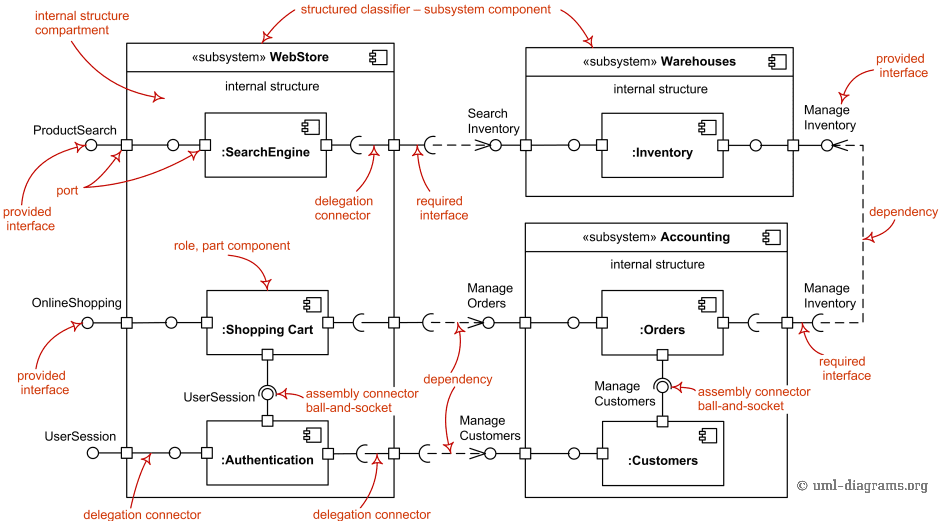
\includegraphics[width=\textwidth]{img/component-diagram.png}
    \caption{Component Diagram.}
\end{figure}

\noindent
To view the component diagram in high resolution, scan (or click) the QR code below.
\begin{center}
    \qrcode{https://github.com/PoliMI-HPC-E-notes-projects-AndreVale69/HPC-E-PoliMI-university-notes/tree/main/software-engineering-for-hpc/notes/img/component-diagram.png}
\end{center}
A complete guide can be found on the following page: \href{https://www.visual-paradigm.com/guide/uml-unified-modeling-language/what-is-component-diagram/}{What is Component Diagram?
}

\newpage

\subsubsection{Sequence Diagram (C\&C structure)}

\definition{Sequence Diagram} show \textbf{elements as they interact over time} and they are organized according to object (horizontally) and time (vertically).

\begin{figure}[!htp]
    \centering
    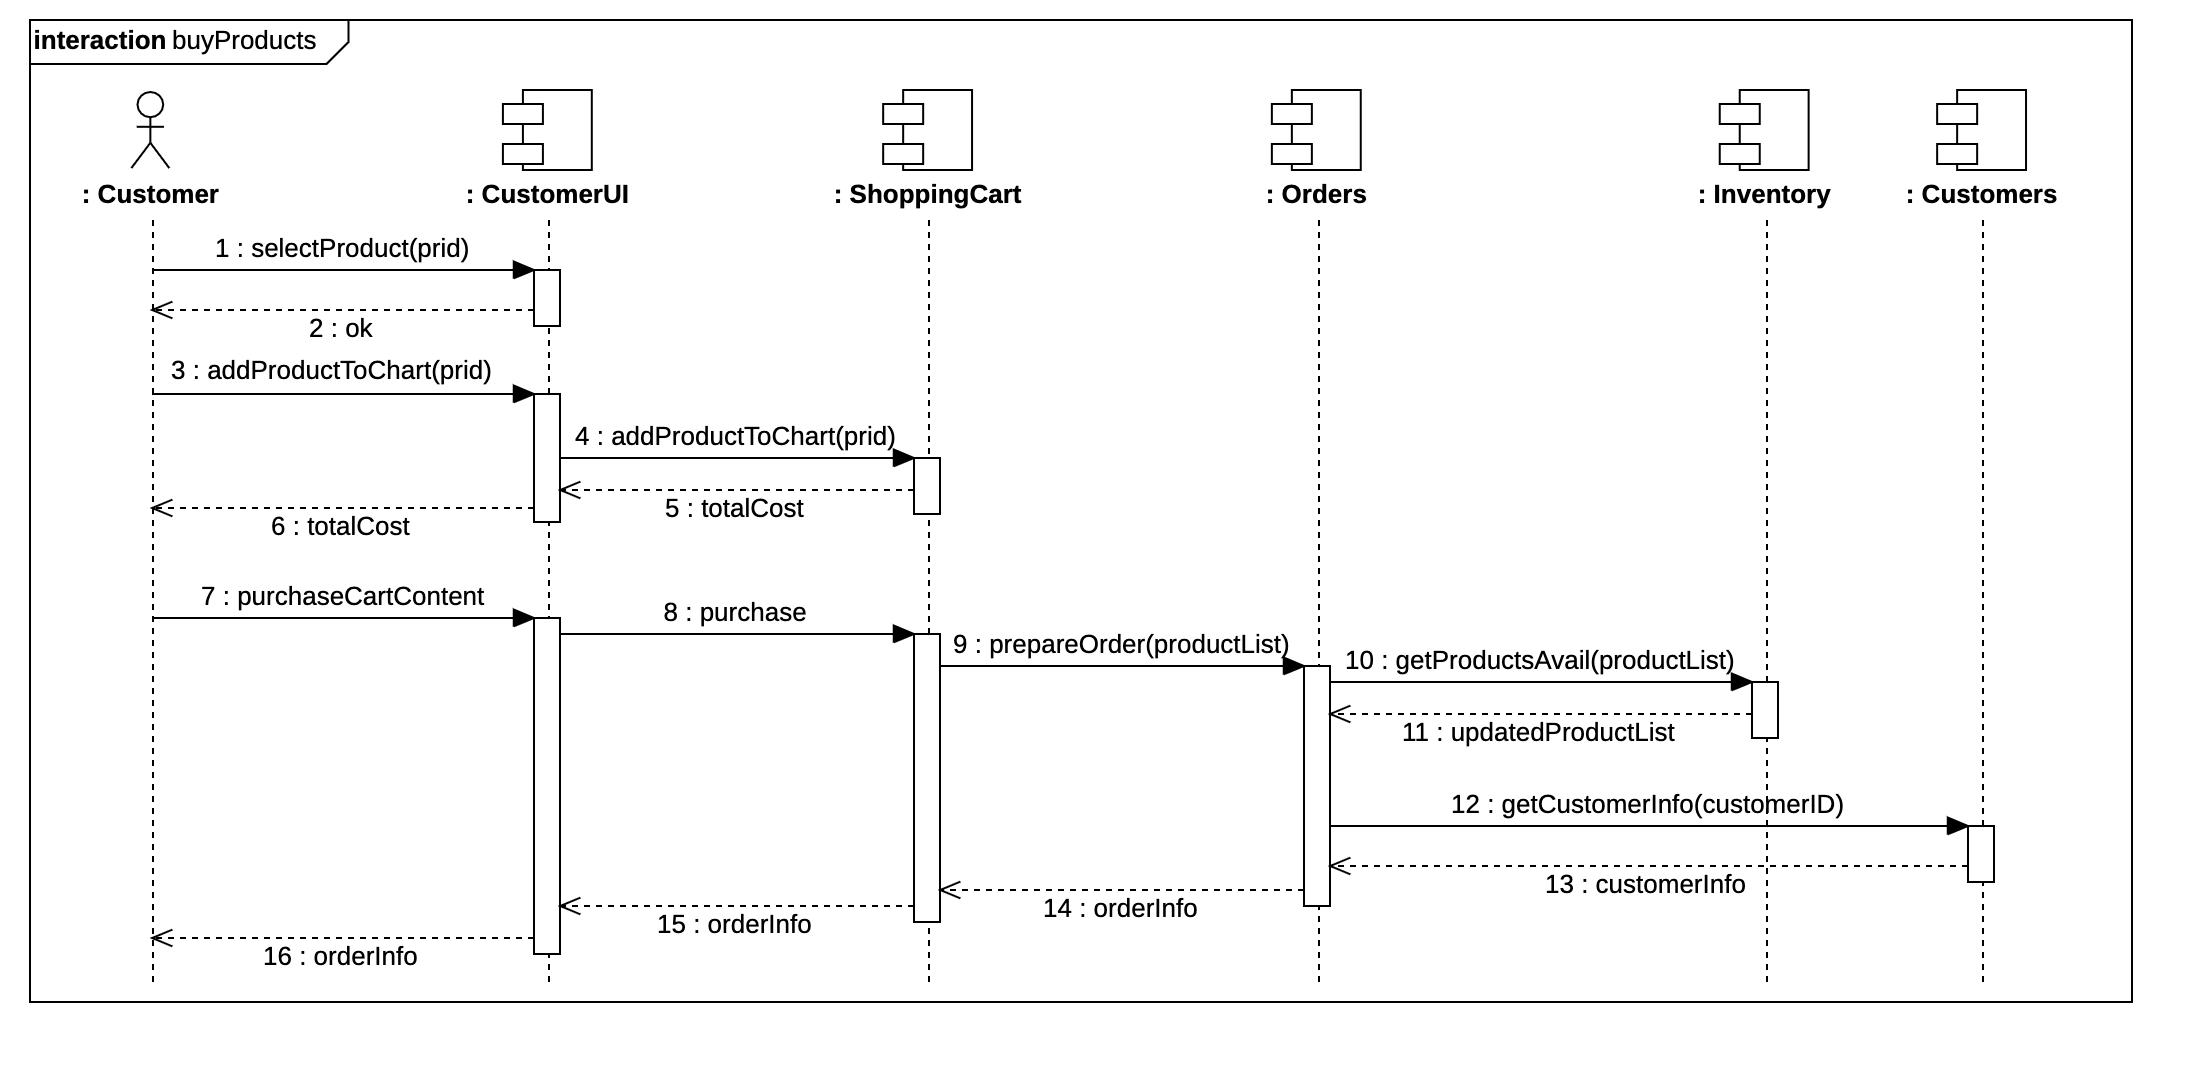
\includegraphics[width=\textwidth]{img/sequence-diagram.png}
    \caption{Sequence Diagram.}
\end{figure}

\noindent
To view the sequence diagram in high resolution, scan (or click) the QR code below.
\begin{center}
    \qrcode{https://github.com/PoliMI-HPC-E-notes-projects-AndreVale69/HPC-E-PoliMI-university-notes/tree/main/software-engineering-for-hpc/notes/img/sequence-diagram.png}
\end{center}
A complete guide can be found on the following page: \href{https://www.visual-paradigm.com/guide/uml-unified-modeling-language/what-is-sequence-diagram/}{What is Sequence Diagram?
}

\newpage

\subsubsection{Class Diagram (module structure)}

A \definition{Class Diagram} is \textbf{a type of static structure diagram} that describes the structure of a system by showing the system's classes, their attributes, operations (or methods), and the relationships among objects.

\begin{figure}[!htp]
    \centering
    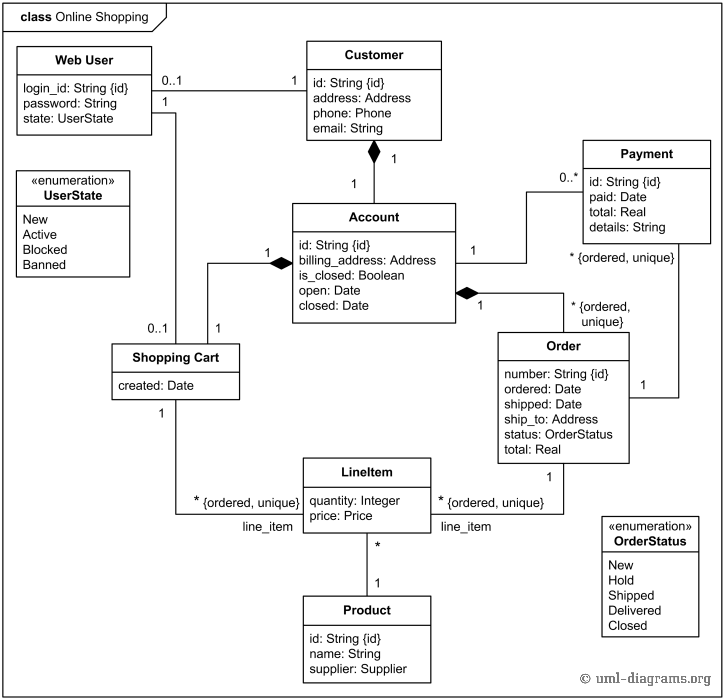
\includegraphics[width=\textwidth]{img/class-diagram.png}
    \caption{Class Diagram.}
\end{figure}

\noindent
To view the sequence diagram in high resolution, scan (or click) the QR code below.
\begin{center}
    \qrcode{https://github.com/PoliMI-HPC-E-notes-projects-AndreVale69/HPC-E-PoliMI-university-notes/tree/main/software-engineering-for-hpc/notes/img/class-diagram.png}
\end{center}
A complete guide can be found on the following page: \href{https://www.visual-paradigm.com/guide/uml-unified-modeling-language/what-is-class-diagram/}{What is Class Diagram?
}

\newpage

\subsubsection{Package Diagram (module structure)}

A \definition{Package Diagram}, a kind of structural diagram, shows the \textbf{arrangement and organization of model elements in middle to large scale project}. Package diagram can show both structure and dependencies between sub-systems or modules, showing different views of a system, for example, as multi-layered (aka multi-tiered) application - multi-layered application model.

\begin{figure}[!htp]
    \centering
    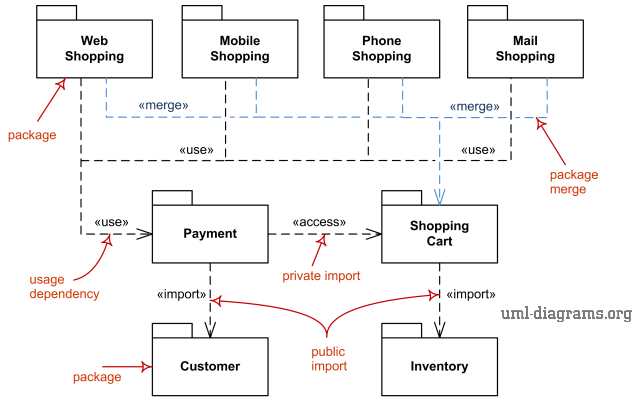
\includegraphics[width=\textwidth]{img/package-diagram.png}
    \caption{Package Diagram.}
\end{figure}

\noindent
To view the sequence diagram in high resolution, scan (or click) the QR code below.
\begin{center}
    \qrcode{https://github.com/PoliMI-HPC-E-notes-projects-AndreVale69/HPC-E-PoliMI-university-notes/tree/main/software-engineering-for-hpc/notes/img/package-diagram.png}
\end{center}
A complete guide can be found on the following page: \href{https://www.visual-paradigm.com/guide/uml-unified-modeling-language/what-is-package-diagram/}{What is Package Diagram?
}

\newpage

\subsubsection{Deployment Diagram (allocation structure)}

A \definition{Deployment Diagram} is a diagram that shows the \textbf{configuration of run time processing nodes and the components that live on them}. Deployment diagrams is a kind of structure diagram used in modeling the physical aspects of an object-oriented system. They are often be used to model the static deployment view of a system (topology of the hardware).

\begin{figure}[!htp]
    \centering
    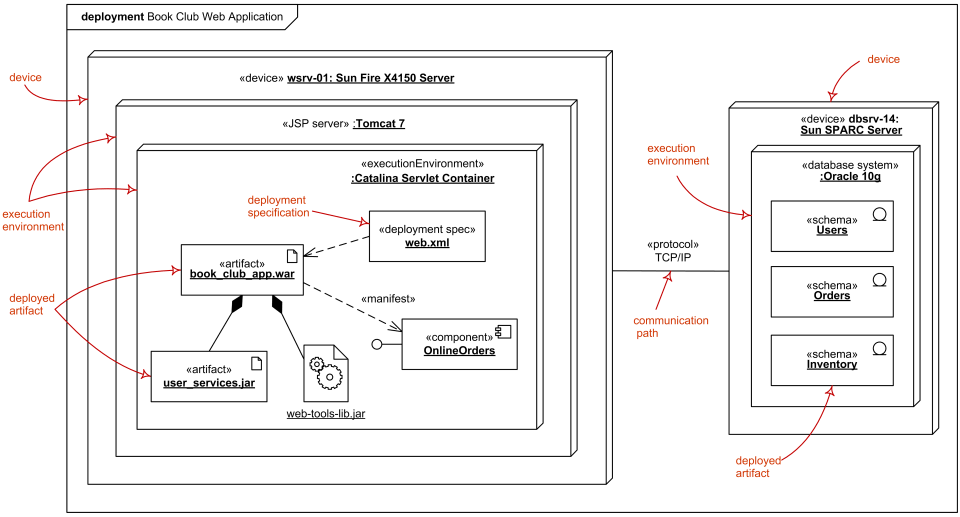
\includegraphics[width=\textwidth]{img/deployment-diagram.png}
    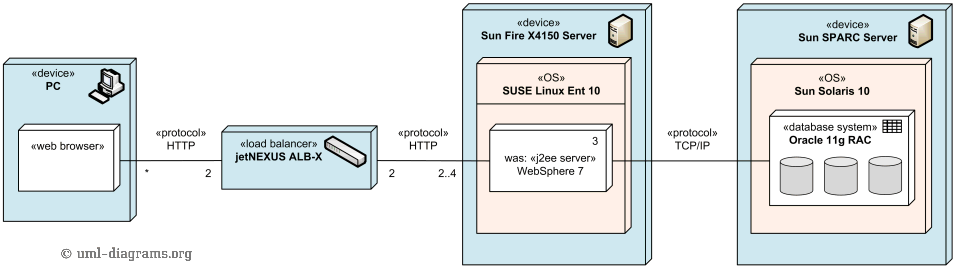
\includegraphics[width=\textwidth]{img/deployment-diagram-2.png}
    \caption{Deployment Diagram.}
\end{figure}

\noindent
To view the sequence diagram in high resolution, scan (or click) the QR code below.
\begin{center}
    \qrcode{https://github.com/PoliMI-HPC-E-notes-projects-AndreVale69/HPC-E-PoliMI-university-notes/tree/main/software-engineering-for-hpc/notes/img/deployment-diagram.png}
    \hspace{2em}
    \qrcode{https://github.com/PoliMI-HPC-E-notes-projects-AndreVale69/HPC-E-PoliMI-university-notes/tree/main/software-engineering-for-hpc/notes/img/deployment-diagram-2.png}
\end{center}
A complete guide can be found on the following page: \href{https://www.visual-paradigm.com/guide/uml-unified-modeling-language/what-is-deployment-diagram/}{What is Deployment Diagram?
}
    \subsection{Design principles}

The following is a list of important design principles in software engineering.

\begin{definitionbox}
    \begin{enumerate}
        \item \textbf{Divide et impera} (also called \emph{divide and conquer})
        
        \item \textbf{Keep the level of abstraction as high as possible}

        \item \textbf{Increase cohesion where possible}

        \item \textbf{Reduce coupling where possible}

        \item \textbf{Design for reusability}

        \item \textbf{Reuse existing designs and code}

        \item \textbf{Design for flexibility}

        \item \textbf{Anticipate obsolescence}

        \item \textbf{Design for portability}

        \item \textbf{Design for testability}

        \item \textbf{Design defensively}
    \end{enumerate}
\end{definitionbox}

\begin{flushleft}
    \large
    \textcolor{Red3}{\textbf{Divide et impera} (\emph{divide and conquer})}
\end{flushleft}
\textbf{Divide and Conquer} is a problem-solving strategy that involves breaking down a complex problem into smaller, more manageable parts, solving each part individually, and then combining the solutions to solve the original problem.

\begin{flushleft}
    \large
    \textcolor{Red3}{\textbf{Keep the level of abstraction as high as possible}}
\end{flushleft}
Ensure that your designs allow you to hide or defer consideration of details, thus reducing complexity. A good abstraction is said to provide \emph{information hiding}. Abstractions allow you to understand the essence of a subsystem without having to know unnecessary details.

    %%%%%%%%%%%%%%%%%%%%%%%
    % Architectural Style %
    %%%%%%%%%%%%%%%%%%%%%%%
    \section{Requirement Engineering}

\subsection{Definition}

Before the definition, we give a possible scenario to understand what requirement engineering is.

\highspace
The municipality of Milan says the following: \dquotes{\emph{The time it takes to make decisions on building permits for residential buildings in the city is too long. We want to develop software that will help us reduce this time}}. So where do we start? How do we identify the most important aspects? How do we make sure that we have understood what our customers want from us?

\begin{definitionbox}
    Software measure engineering (\definition{Requirement Engineering}) is the process of discovering the purpose for which the software is intended by identifying stakeholders and their needs, and documenting these in a form suitable for analysis, communication and subsequent implementation.
\end{definitionbox}

\noindent
The questions derived from requirements engineering are:
\begin{itemize}
    \item Identify stakeholders
    \item Identify their needs
    \item Produce documentation
    \item Analyze, communicate, implement requirements
\end{itemize}

\begin{figure}[!htp]
    \centering
    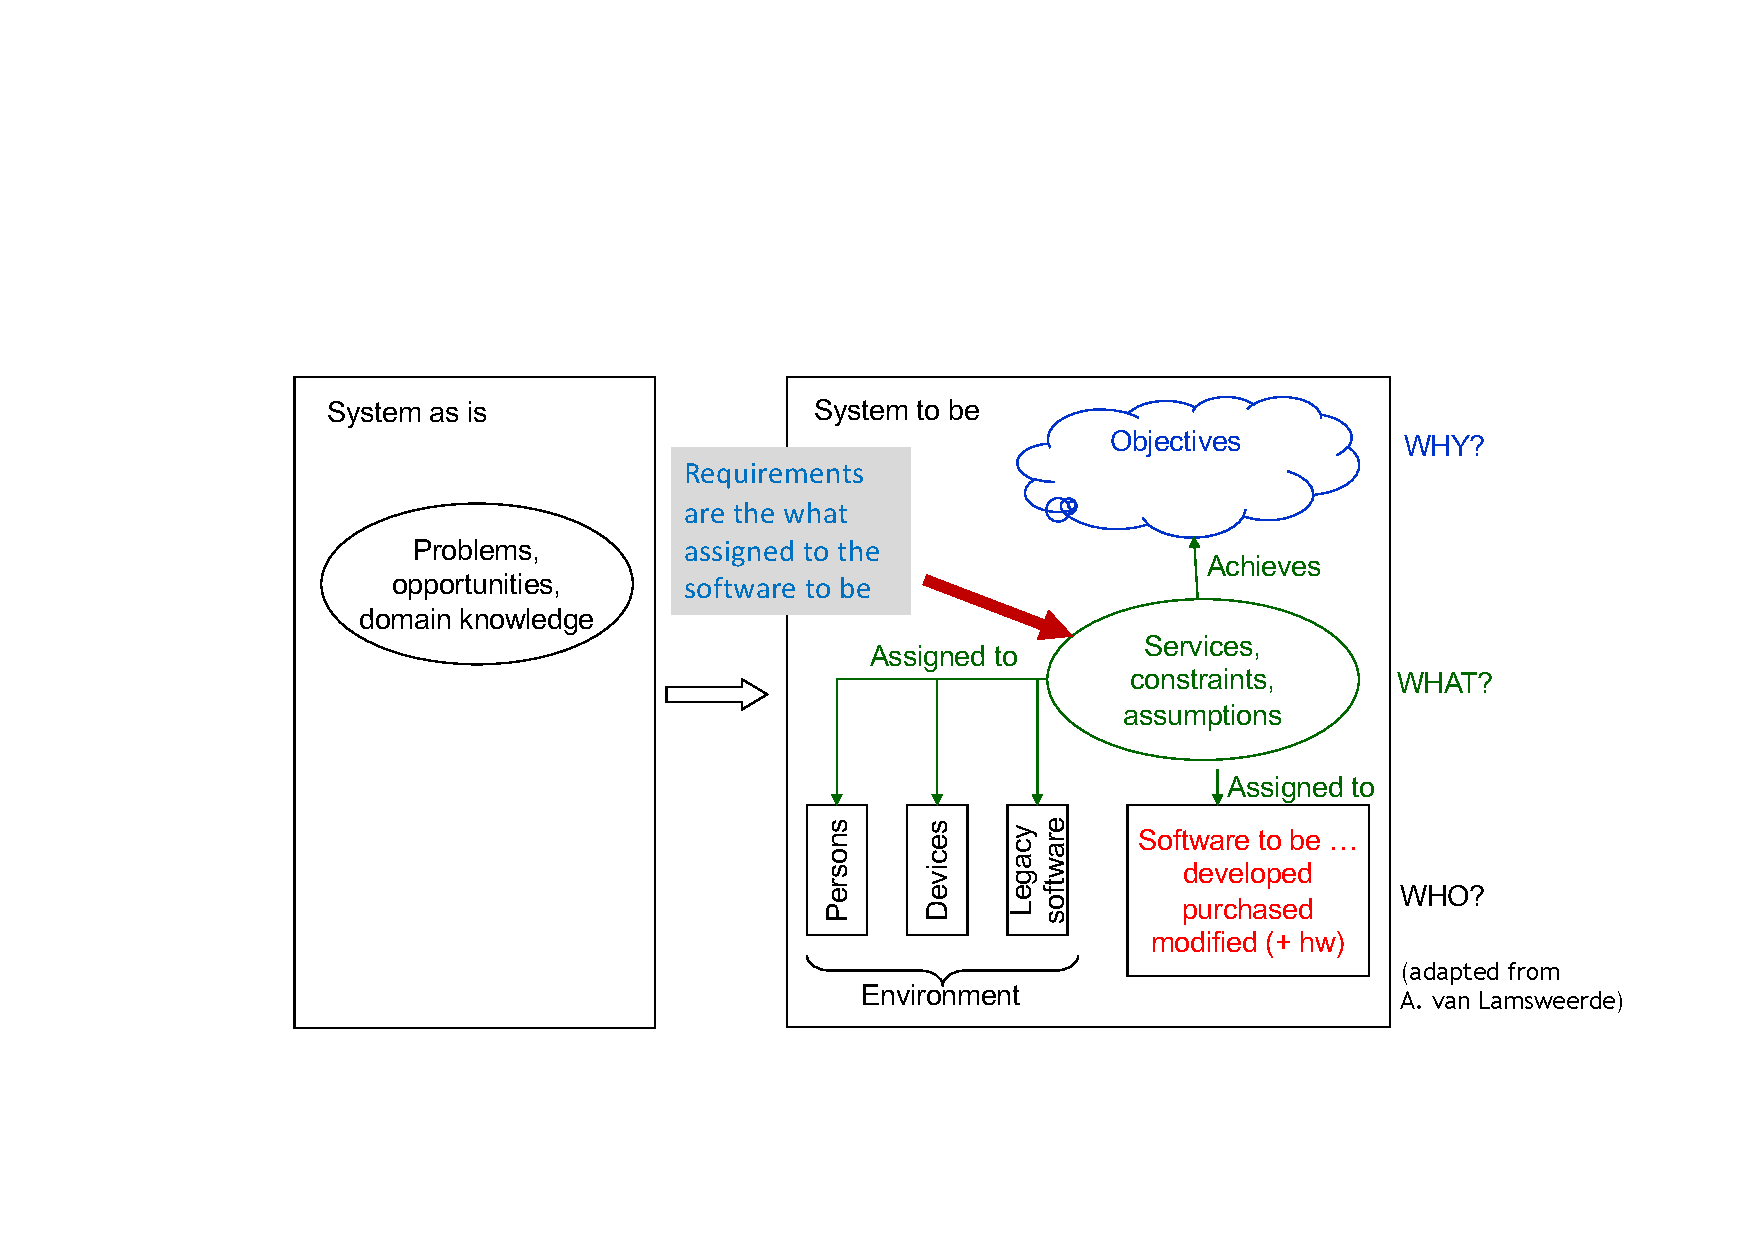
\includegraphics[width=\textwidth]{img/requirement-engineering-1.pdf}
    \caption{Analyzing the system as is and the system to be.}
\end{figure}
    \subsection{Client-Server}

A \definition{Client-Server Architecture} is a \textbf{network-based computing structure} where responsibilities and operations get \textbf{distributed between clients and servers}. Client-Server Architecture is widely used for network applications such as email, web, online banking, e-commerce, etc.

\begin{flushleft}
    \textcolor{Green3}{\textbf{\faIcon{check} When to use it}}
\end{flushleft}
The three most common cases are:
\begin{itemize}
    \item When \textbf{multiple users} need to access a \textbf{single resource} (e.g. database).

    \item When there is a preexisting software and we must \textbf{access remotely} (e.g. email server).
    
    \item When it is convenient to organize the system around a \textbf{shared piece of functionality used by multiple components} (e.g. authentication or authorization server).
\end{itemize}

\begin{flushleft}
    \textcolor{Red2}{\textbf{\faIcon{exclamation-triangle} Technical issues}}
\end{flushleft}
With this architecture, it's necessary to \textbf{design} and \textbf{document} proper \textbf{interfaces} for our server. It is also necessary to ensure that the server can \textbf{handle multiple simultaneous requests}.

\subsubsection{Interface design}

An \definition{interface design} is a \textbf{boundary} across which components interact. Proper definition of interfaces is an architectural concern (affects maintainability, usability, testability, performance, integrability). There are two important \textbf{guiding principles} for interface design: \textbf{information hiding} and \textbf{low coupling}. An interface should encapsulate a component implementation so that it can be changed without affecting other components.

\highspace
There are several aspects to interface design that need to be considered:
\begin{itemize}
    \item \definition{Contract principle}: any resource (operation, data) added to an interface implies a \textbf{commitment to maintaining} it.

    \item \definition{Least surprise principle}: interfaces should \textbf{behave} consistently \textbf{with expectations}.

    \item \definition{Small interfaces principle}: interfaces should limit the \textbf{exposed resources to the minimum}.
\end{itemize}
There are also some important elements to define: \textbf{interaction style} (e.g. sockets, RPC, REST); \textbf{representation} and structure of exchanged data (affecting expressiveness, interoperability, performance and transparency); \textbf{error handling}.

\newpage

\subsubsection{Error handling, multiple interfaces and interface evolution}

Sometimes there may be some problems, for example: an operation is called with invalid parameters and consequently the call doesn't return anything. This simple example can provoke some scenarios: the component cannot handle the request in its current state; or hardware/software errors prevent successful execution; or there is a misconfiguration issue (e.g. the server is not correctly connected to the database).

There are three possible \textbf{solutions}: \textbf{raising an exception}; \textbf{return an error code} (common); \textbf{log the problem}. There's no single solution, but we can choose several (e.g. error code and log the problem).

\highspace
A \textbf{server} can offer \definition{multiple interfaces} at the same time. This enables separation of concerns, different levels of access rights and support ot \textbf{interface evolution}.

\highspace
\textbf{Interface evolution} occurs for many reasons (e.g. to support new requirements). Several \textbf{strategies} are needed to support continuity:
\begin{itemize}
    \item \textbf{\underline{Deprecation}}: declare well in advance that an interface version will be retired by a certain date;

    \item \textbf{\underline{Versioning}}: maintain multiple active versions of the interface;

    \item \textbf{\underline{Extension}}: a new version extends the previous one.
\end{itemize}

\newpage

\subsubsection{Handling multiple requests}

The server must be able to receive and process requests from multiple clients. There are two main approaches to this: \emph{forking} and \emph{worker pooling}.

\begin{flushleft}
    \large
    \textcolor{Red2}{\textbf{Forking}}
\end{flushleft}
The \definition{forking} approach is the same as that used by the Apache Web Server: \textbf{one process per request or per client}.

\begin{figure}[!htp]
    \centering
    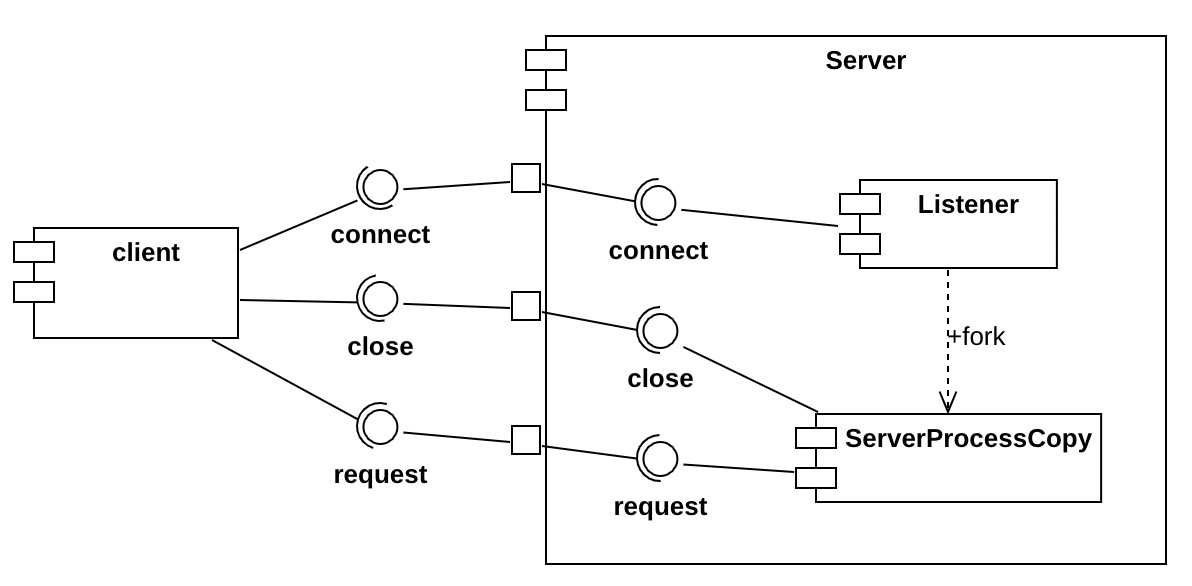
\includegraphics[width=.8\textwidth]{img/forking-1.png}
    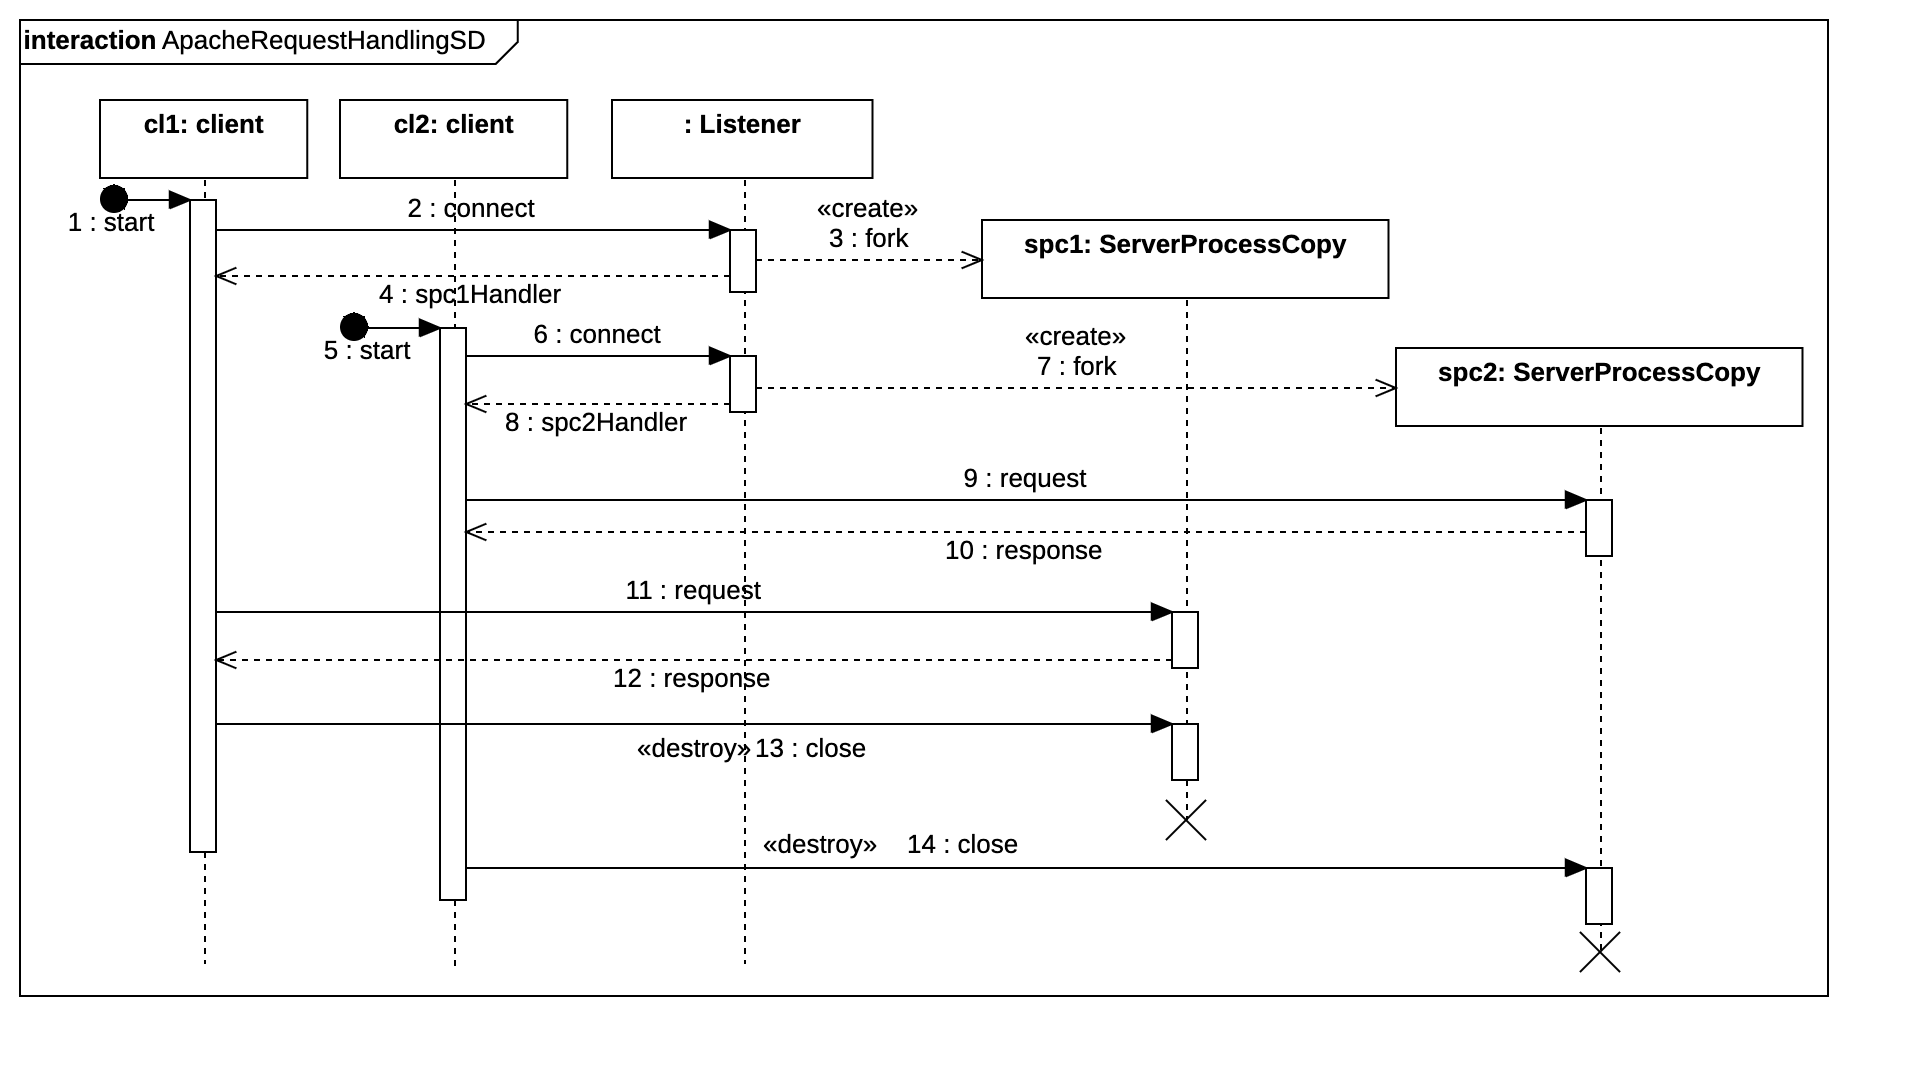
\includegraphics[width=\textwidth]{img/forking-2.png}
    \caption{Forking diagrams.}
\end{figure}

\begin{flushleft}
    \textcolor{Green3}{\textbf{\faIcon{check} Forking Advantages}}
\end{flushleft}
\begin{itemize}
    \item Architectural \textbf{simplicity}.
    
    \item \textbf{Isolation} and \textbf{protection} given by the one-connection-per-process model. Note: slow processes do not affect other incoming connections.
    
    \item \textbf{Simple to program}.
\end{itemize}

\newpage

\begin{flushleft}
    \textcolor{Red2}{\textbf{\faIcon{exclamation-triangle} Forking Issues}}
\end{flushleft}
\begin{itemize}
    \item Growth of the WWW over the last 20 years (number of users and weight of web pages).
    
    \item The number of \textbf{active processes} at time $t$ is \textbf{difficult to predict} and may \textbf{saturate resources}.
    
    \item \textbf{Expensive} fork-kill operations for each \textbf{incoming connection}.
\end{itemize}

\newpage

\begin{flushleft}
    \large
    \textcolor{Red2}{\textbf{Worker pooling}}
\end{flushleft}
It is an alternative approach adopted by NGINX Web Server. It is \textbf{designed for high concurrency} but has to deal with \textbf{scalability issues}.

\begin{figure}[!htp]
    \centering
    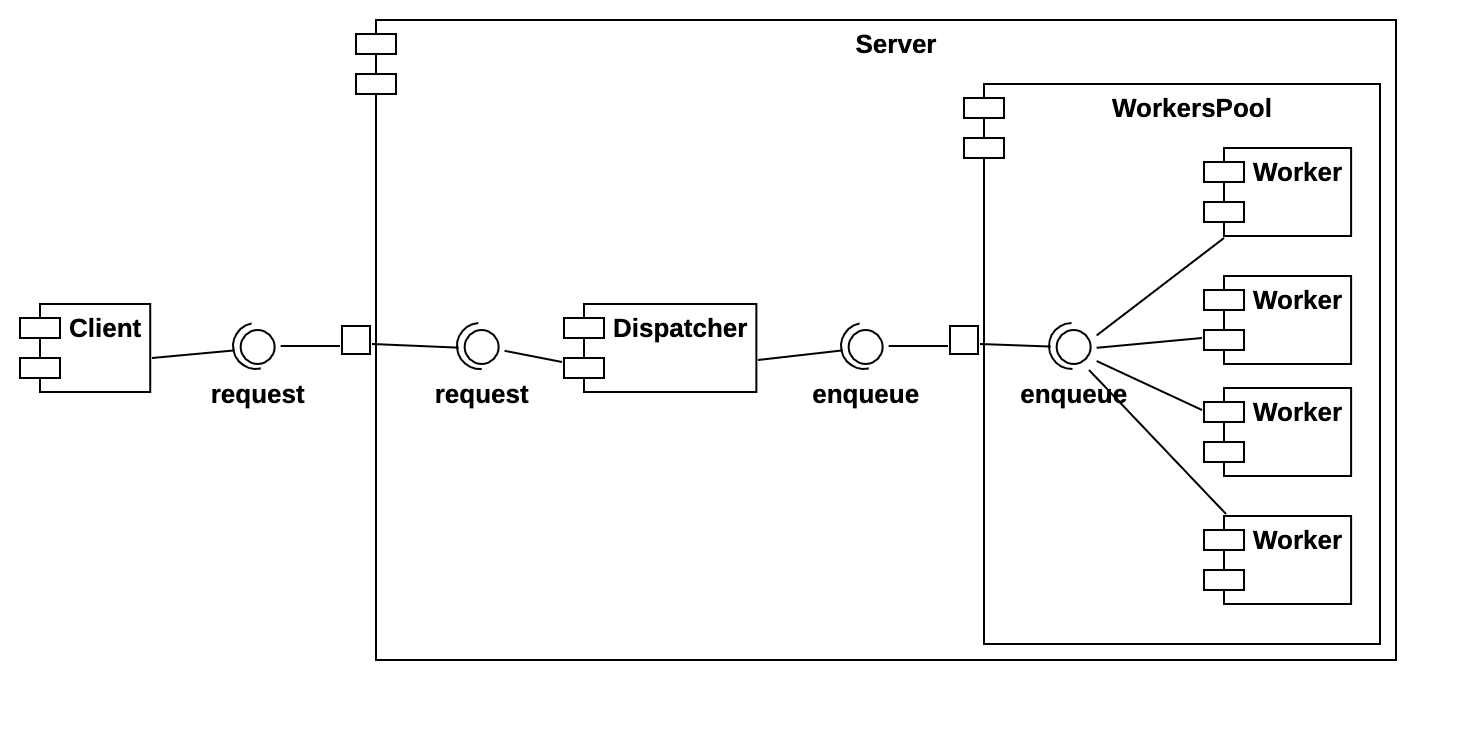
\includegraphics[width=.9\textwidth]{img/worker-pooling-1.png}
    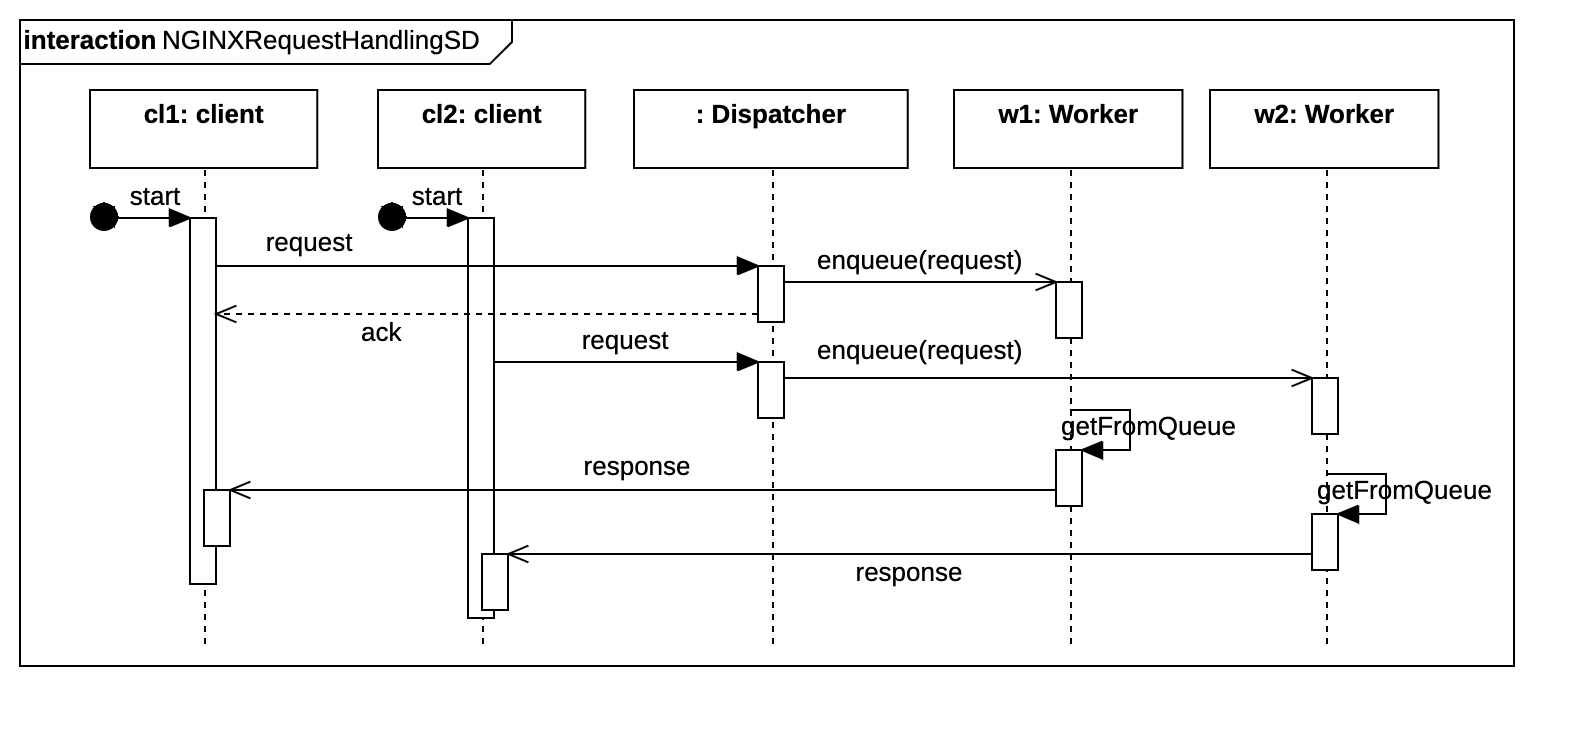
\includegraphics[width=\textwidth]{img/worker-pooling-2.png}
    \caption{Worker pooling diagrams.}
\end{figure}

\noindent
Despite the well-known problem of this architecture (scalability), NGINX addresses the previous problems by introducing a new \textbf{architectural tactic}. A \emph{tactic} is a \textbf{design decision that affects the control of one or more quality attributes}.

\begin{flushleft}
    \textcolor{Green3}{\textbf{\faIcon{check} Worker Pooling Advantages (quality attribute trade-offs)}}
\end{flushleft}
\begin{itemize}
    \item Number of \textbf{workers} is fixed, so they \textbf{do not saturate available resources}.
    
    \item \textbf{Each worker} has a \textbf{queue}.
    
    \item When \textbf{queues} are \textbf{full} the \textbf{dispatcher drops the incoming requests} to keep high performance (\textbf{optimize scalability and performance by sacrificing availability}).
    
    \item Dispatcher \textbf{balances} the \textbf{workload} among available workers \textbf{according to specific policies}.
\end{itemize}
    \subsection{Three-Tier Architecture}

The following is a summary of the \href{https://www.ibm.com/topics/three-tier-architecture}{IBM guide}.

\highspace
\definition{Three-tier architecture} is a well-established software application architecture that \textbf{organizes applications into three logical and physical computing tiers}: 
\begin{itemize}
    \item The \textbf{presentation} tier, or user interface;
    
    \item The \textbf{application} tier, where data is processed;
    
    \item The \textbf{data} tier, where application data is stored and managed.
\end{itemize}

\begin{flushleft}
    \textcolor{Green3}{\textbf{\faIcon{check} Benefits}}
\end{flushleft}
The chief benefit of three-tier architecture is its \textbf{logical and physical separation} of functionality. Each tier can run on a separate operating system and server platform - for example, web server, application server, database server - that best fits its functional requirements. And each tier runs on at least one dedicated server hardware or virtual server, so the services of \textbf{each tier can be customized and optimized without impacting the other tiers}. Other benefits include:
\begin{itemize}
    \item \textbf{Faster development}: Because \emph{each tier can be developed simultaneously by different teams}, an organization can bring the application to market faster. And programmers can use the latest and best languages and tools for each tier.
    
    \item \textbf{Improved scalability}: \emph{Any tier can be scaled independently} of the others as needed.

    \item \textbf{Improved reliability}: An outage in one tier is less likely to impact the availability or performance of the other tiers.

    \item \textbf{Improved security}: Because the \emph{presentation tier and data tier can't communicate directly}, a well-designed application tier can function as an internal firewall, preventing SQL injections and other malicious exploits.
\end{itemize}

\subsubsection{N-tier architecture}

\definition{N-tier architecture} (also called or multitier architecture) refers to any application architecture with \textbf{more than one tier}. But applications with more than three layers are \underline{rare} because extra layers offer \textbf{few benefits} and can make the \textbf{application slower}, \textbf{harder to manage} and \textbf{more expensive to run}. As a result, n-tier architecture and multitier architecture are usually synonyms for three-tier architecture.
    \subsection{Microservice architectural style}

The microservice architectural style is an approach to developing a single application as a suite of \textbf{small services}, each running in its own process and communicating \textbf{lightweight mechanisms}, often an HTTP resource API.

\begin{flushleft}
    \textcolor{Green3}{\textbf{\faIcon{check} Benefits}}
\end{flushleft}
There are two main benefits:
\begin{itemize}
    \item \textbf{Technology heterogeneity}. \textbf{Each service uses its own technology stack}. The technology stack can be selected to fit the task best (e.g. data analysis vs video streaming). The teams can experiment with new technologies within a single microservice (e.g. we can deploy two versions and do A/B testing). Also, no unnecessary dependencies or libraries for each service.
    
    \item \textbf{Scaling}. \textbf{Each microservice can be scaled independently}. Also, identified bottlenecks can be addressed directly. Parts of the system that do not represent bottlenecks can remain simple and unscaled.
\end{itemize}
    \subsection{Event-Driven Architecture}

An \definition{Event-Driven Architecture} uses \textbf{events to trigger and communicate between decoupled services} and is common in modern applications built with microservices. An event is a change in state, or an update, like an item being placed in a shopping cart on an e-commerce website. Events can either carry the state (the item purchased, its price, and a delivery address) or events can be identifiers (a notification that an order was shipped).

Often it's called \textbf{publish-subscribe} (publish is the event generation, and subscribe is the declaration of the interest).

\begin{flushleft}
    \textcolor{Green3}{\textbf{\faIcon{check} Benefits}}
\end{flushleft}
\begin{itemize}
    \item \textbf{Very common in modern development practices} (e.g. continuous integration and deployment, such as GitHub Actions).

    \item \textbf{Easy addition/deletion of components} (publishers and subscribers are decoupled; the event dispatcher handles this dynamic set).
\end{itemize}

\begin{flushleft}
    \textcolor{Red2}{\textbf{\faIcon{exclamation-triangle} Problems}}
\end{flushleft}
\begin{itemize}
    \item \textbf{Potential scalability problems} (the event dispatcher may become a bottleneck under high workload).
    
    \item \textbf{Ordering of events} (not guaranteed, not straightforward).
\end{itemize}

\highspace
Other characteristics of this architecture:
\begin{itemize}
    \item THe messages and the events are \textbf{asynchronous}.
    
    \item Computation is \textbf{reactive} (driven by receipt of message).

    \item \textbf{Destination} of messages \textbf{determined by receiver}, not sender (location/identity abstraction).

    \item \textbf{Loose coupling} (senders and receivers added without reconfiguration).
    
    \item \textbf{Flexible} communication means (one-to-many, many-to-one, many-to-many).
\end{itemize}
Some \example{examples} of relevant technologies are: \href{https://kafka.apache.org/}{Apache Kafka} and \href{https://www.rabbitmq.com/}{RabbitMQ}.

\newpage

\subsubsection{Apache Kafka}

\definition{Kafka} is a \textbf{framework} for the event-driven paradigm:
\begin{itemize}
    \item Includes primitives to create \textbf{event produces} and \textbf{consumers} and a runtime infrastructure to handle \textbf{event transfer} from producers to consumers.
    
    \item \textbf{Stores events} durably and reliably.
    
    \item Allow consumers to \textbf{process events} as they occur or retrospectively.
\end{itemize}
These services are offered in a distributed, highly scalable, elastic, fault-tolerant, and secure manner.

\begin{figure}[!htp]
    \centering
    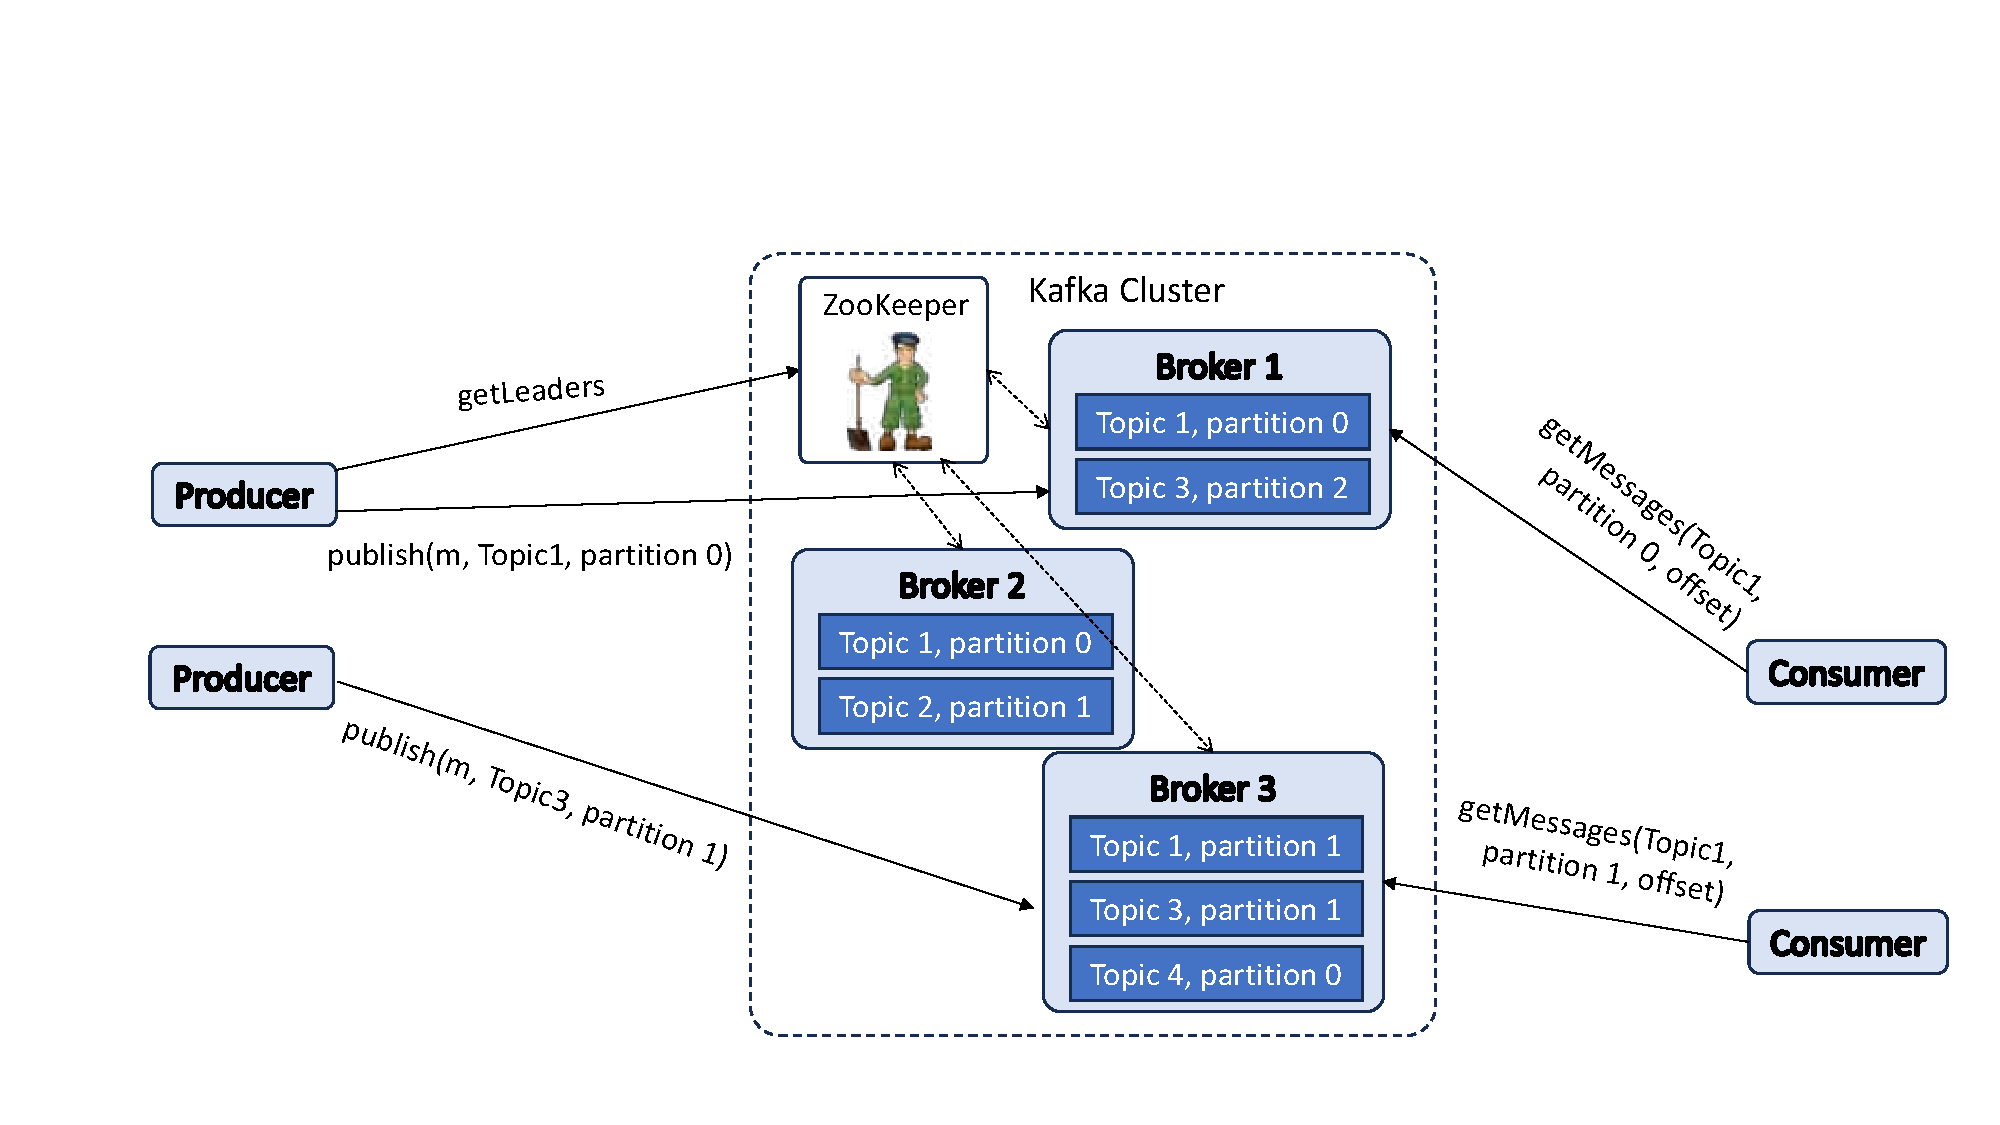
\includegraphics[width=\textwidth]{img/kafka-arch-1.pdf}
    \caption{Kafka architecture (the ZooKeeper is a \dquotes{health manager}).}
\end{figure}

\noindent
Some important features:
\begin{itemize}
    \item Each \textbf{broker} handles a set of \textbf{topics} and \textbf{topic partitions}, parts including sets of messages on the topic.

    \item The \emph{partitions} are independent from each other and can be \textbf{replicated} on multiple brokers for fault tolerance.

    \item There is \textbf{one leading broker per partition}. The other brokers containing the same partition are \textbf{followers}.
    
    \item The \textbf{producers} know the available leading brokers and send messages to them.
    
    \item \textbf{Messages in the same topic} are organized in \textbf{batches} at the producers' side and then sent to the broker when the batch size overcomes a certain threshold.

    \item \textbf{Consumers} adopt a \textbf{pull approach}. They \emph{receive in a single batch all messages} belonging to a certain partition starting from a specified offset.

    \item \textbf{Messages} remain \textbf{available} at the brokers' side \textbf{for a specified period} and can be \textbf{read multiple times} in this period.
    
    \item The leader keeps track of the \textbf{in-synch followers}.
    
    \item \textbf{ZooKeeper is used to monitor the correct operation of the cluster}. All brokers send heartbeats to ZooKeeper. ZooKeeper will replace a failed broker by electing a new leader for all partitions that the failed broker was leading. It can also start/restart brokers.
\end{itemize}

\begin{center}
    \large
    \textcolor{Red2}{\textbf{Message delivery}}
\end{center}

\begin{flushleft}
    \textcolor{Red2}{\textbf{Producer}}
\end{flushleft}
\begin{enumerate}
    \item Brokers commit messages by storing them in the corresponding partition;
    
    \item Leader adds the message to followers (replicas) if available.
\end{enumerate}

\begin{figure}[!htp]
    \centering
    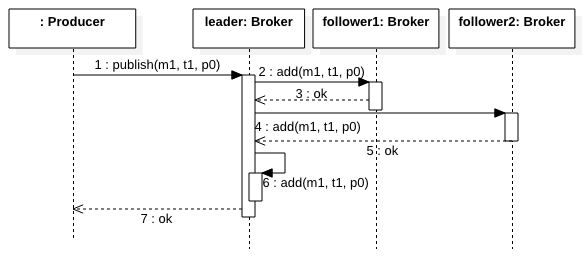
\includegraphics[width=\textwidth]{img/kafka-producer.png}
    \caption{Sequence diagram Kafka producer.}
\end{figure}

\noindent
A possible \textbf{issue}: in case of failure, the \textbf{producer may not get the response} (message number 7 in figure). In this case, the producer has to resend the message and kafka brokers can identify and eliminate duplicates.

\highspace
Synchronization with replicas can be transactional and it's possible to choose between the following options:
\begin{itemize}
    \item \textbf{Exactly-once} semantics is possible but long waiting time. So \textbf{replicas are not allowed}, but the problem is that Kafka spent a \textbf{long time trying to guarantee uniqueness}.

    \item \textbf{At-least-once} can be chosen by excluding duplicates' management.

    \item \textbf{At-most-once} can be chosen by publishing messages asynchronously.
\end{itemize}

\begin{flushleft}
    \textcolor{Red2}{\textbf{Consumer}}
\end{flushleft}
Each \textbf{consumer} can rely on a \textbf{persistent log} to keep track of the \textbf{offset} so that it is not lost in case of failure.

\highspace
\textbf{Issue} case: if the consumer fails after having elaborated messages and before storing the new offset in the log, the same messages will be retrieved again (\textbf{at-least-once semantics}). Note that the delivery semantics can be changed if the new offset is store before the elaboration and we can choose \textbf{at-most-once semantics} because, if failing after storing the offset, the effect of the received messages does not materialize. Finally, transactional management of the log also allows for \textbf{exactly-once semantics}.

\begin{figure}[!htp]
    \centering
    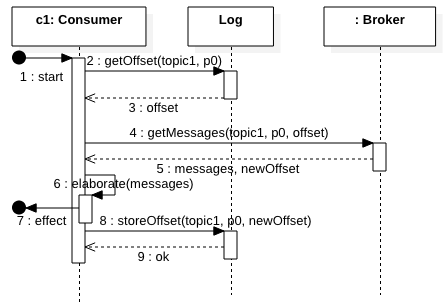
\includegraphics[width=.8\textwidth]{img/kafka-consumer.png}
    \caption{Sequence diagram Kafka consumer.}
\end{figure}

\begin{center}
    \large
    \textcolor{Red2}{\textbf{Kafka architectural tactics}}
\end{center}
There are some tactics used to improve some features of Kafka. In the following section we can see scalability and fault tolerance.

\begin{flushleft}
    \textcolor{Red2}{\textbf{Improve Scalability}}
\end{flushleft}
By \textbf{creating multiple partitions and multiple brokers}, we can create the ability to distribute producers/consumers to different partitions handled by different brokers. We can also \textbf{scale the operations} because Kafka supports the \textbf{creation of clusters of brokers}. Consider that each cluster contains up to a hundred brokers capable of handling trillions of messages per day.

\begin{flushleft}
    \textcolor{Red2}{\textbf{Improve Fault Tolerance}}
\end{flushleft}
By \textbf{creating partitions}, we use the \textbf{persistence} of the partitions. \textbf{Replication} also reduces the risk of data loss. Finally, cluster management takes care of restarting brokers and setting leaders as needed.
    \subsection{Data-Intensive applications}

Before we introduce the architectural styles for data-intensive applications, we explain the difference between batch and stream processing.

\highspace
\definition{Batch processing} is a method of running software programs called jobs in batches automatically. While users are required to submit the jobs, no other interaction by the user is required to process the batch.

\highspace
\definition{Stream processing} (also known as event stream processing, data stream processing, or distributed stream processing) is a programming paradigm which views streams, or sequences of events in time, as the central input and output objects of computation.

\begin{table}[!htp]
    \centering
    \begin{tabular}{@{} p{16em} p{16em} @{}}
        \toprule
        \textbf{Batch} & \textbf{Stream} \\
        \midrule
        Has access to all data. & Computes a function of one data element, or a smallish window of recent data. \\
        \cmidrule{1-2}
        Might compute something big and complex. & Computes something relatively simple. \\
        \cmidrule{1-2}
        Is generally more concerned with throughput than latency of individual components of the computation. & Needs to complete each computation in near-real-time - probably seconds at most. \\
        \cmidrule{1-2}
        Has latency measured in minutes or more. & Computations are generally independent. \\
        \cmidrule{1-2}
        & Asynchronous - source of data doesn't interact with the stream processing directly, like by waiting for an answer. \\
        \bottomrule
    \end{tabular}
    \caption{Batch vs Stream processing.}
\end{table}
    \subsubsection{Batch approach: MapReduce}

\definition{MapReduce} is a \textbf{programming architecture} and an associated implementation for processing and generating big data sets with a parallel, distributed algorithm on a cluster.

\highspace
A MapReduce is composed of a \textbf{map procedure}, which performs filtering and sorting (such as sorting students by first name into queues, one queue for each name), and a \textbf{reduce method}, which performs a summary operation (such as counting the number of students in each queue, yielding name frequencies). The \dquotes{MapReduce System} (also called \dquotes{infrastructure} or \dquotes{framework}) orchestrates the processing by marshalling the distributed servers, running the various tasks in parallel, managing all communications and data transfers between the various parts of the system, and providing for redundancy and fault tolerance.

\begin{examplebox}[: an example of a batch approach using MapReduce]
    \begin{center}
        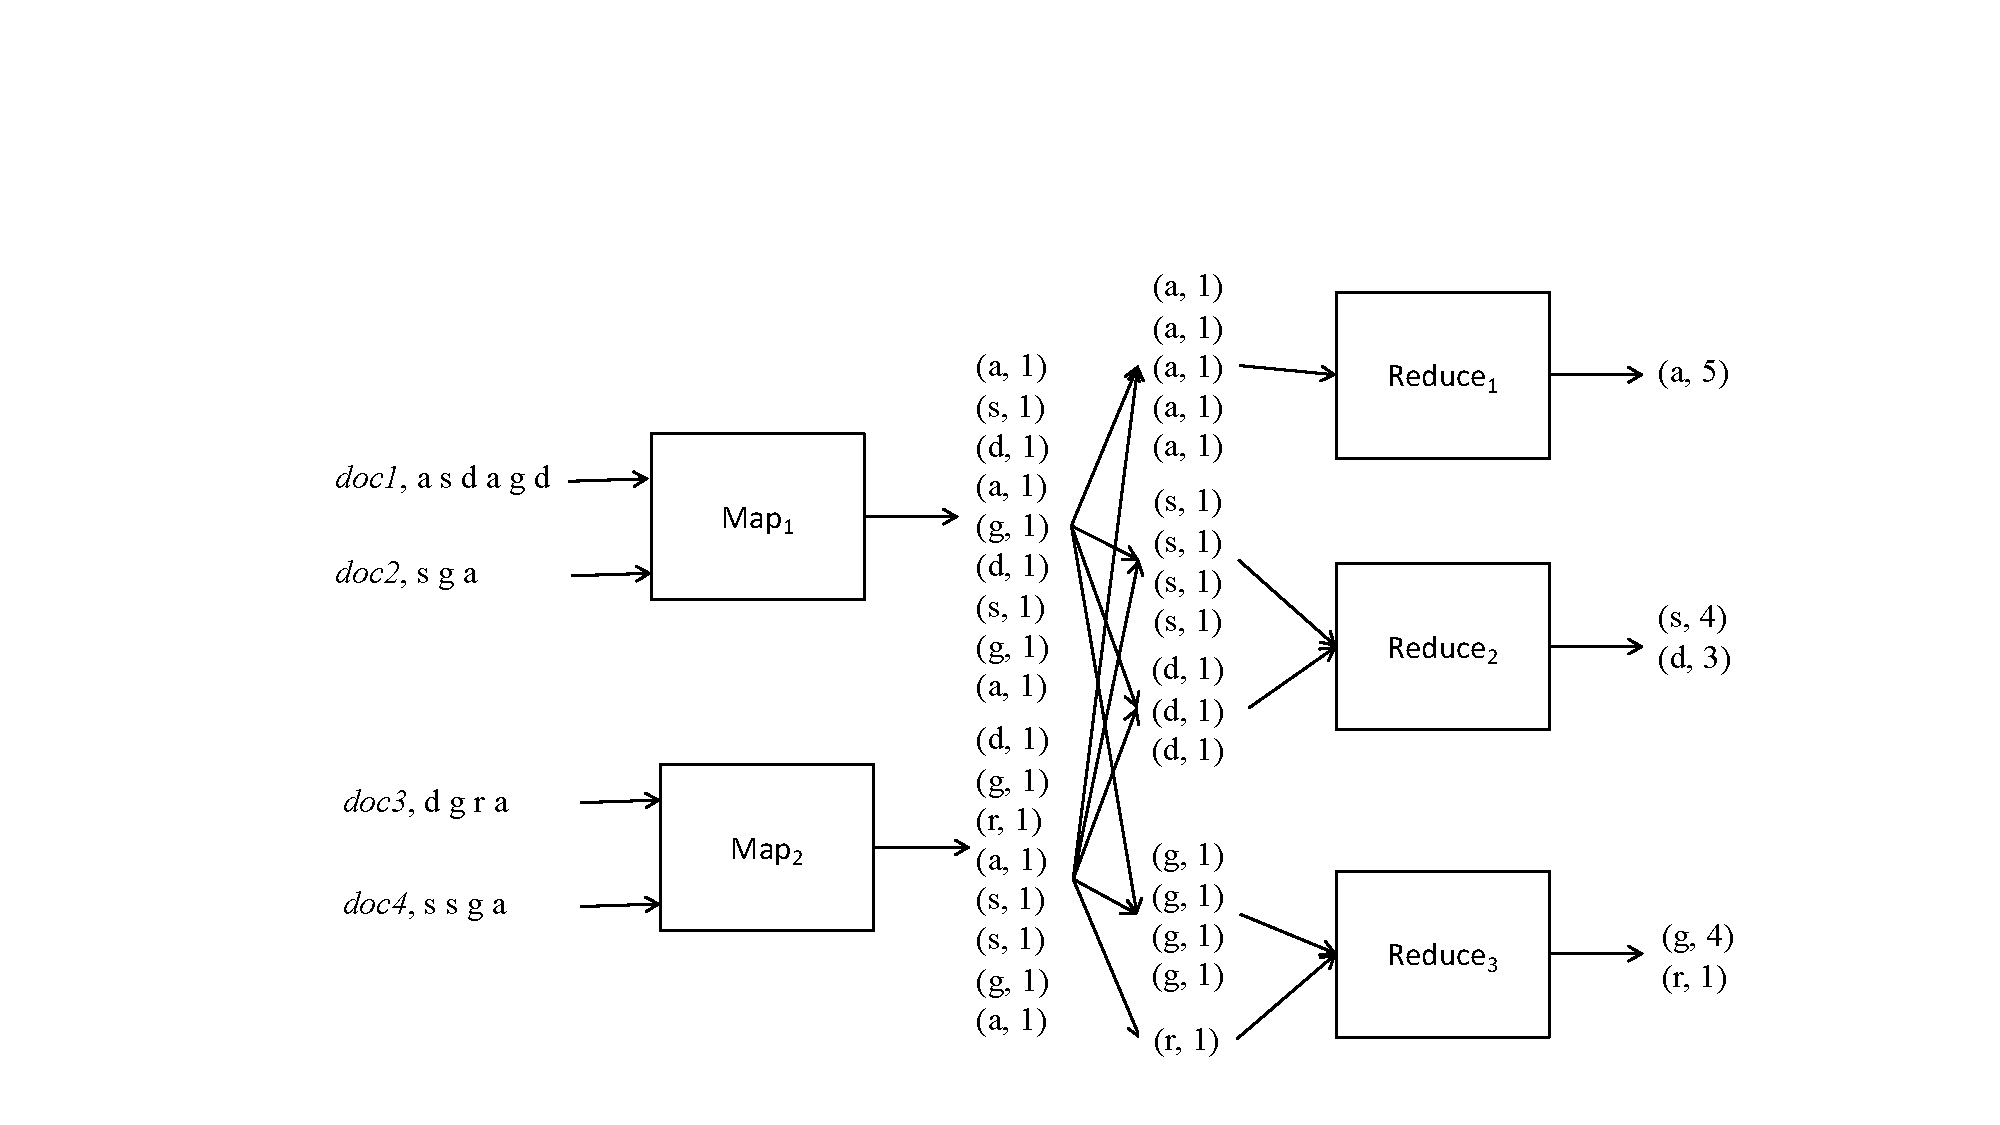
\includegraphics[width=\textwidth]{img/mapreduce-1.pdf}
    \end{center}
    The workflow is the following:
    \begin{enumerate}
        \item Read a set of input files and break it into records;
        
        \item Call the \texttt{map} function. It extracts a key and a value from each record (the assigned value is application-dependent);

        \item Sort all the key-value pairs by key;
        
        \item Call the reduce function. It iterates over the ordered sets of key-value pairs and combines the values (the combination logic is application-dependent)
    \end{enumerate}
\end{examplebox}

\newpage

\begin{figure}[!htp]
    \centering
    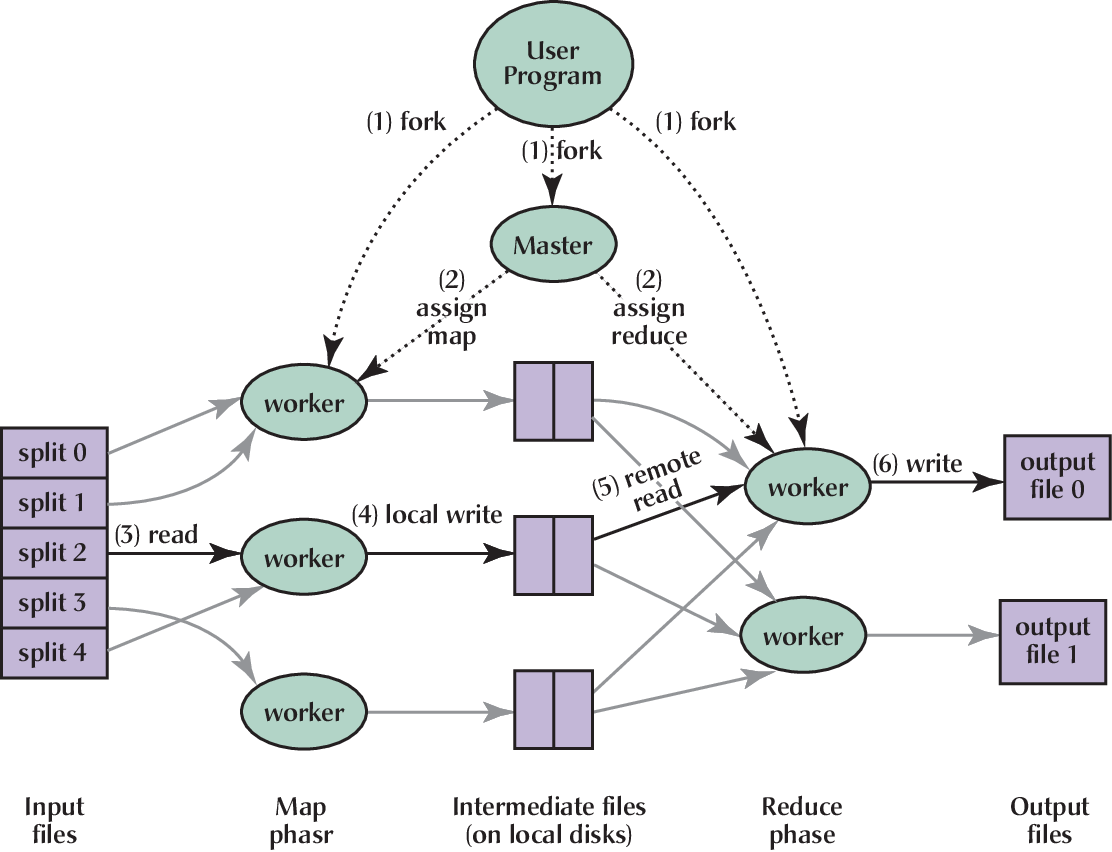
\includegraphics[width=\textwidth]{img/mapreduce-2.png}
    \caption{MapReduce architecture.}
\end{figure}

\begin{flushleft}
    \textcolor{Green3}{\textbf{\faIcon{check} Advantages}}
\end{flushleft}
\begin{itemize}
    \item Works well on commodity hardware.\footnote{Commodity hardware in computing is computers or components that are readily available, inexpensive and easily interchangeable with other commodity hardware. Almost all PCs use commodity hardware.}
\end{itemize}

\begin{flushleft}
    \textcolor{Red2}{\textbf{\faIcon{exclamation-triangle} Disadvantages}}
\end{flushleft}
\begin{itemize}
    \item Implementing a complex processing job is not simple (high level programming model have been built on top of it);

    \item Reducers have to wait until the preceding Mappers have concluded their job;

    \item Materialization of intermediate states can be overkilling;

    \item Sometimes it is not necessary to sort the results of mappers;

    \item New batch computation approaches supported by frameworks as Spark, Tez, Flink, etc.
\end{itemize}
    \subsubsection{Stream approach: Apache Storm}

\definition{Apache Storm} is a \textbf{distributed stream processing computation framework} written predominantly in the Clojure programming language. Originally created by Nathan Marz and team at BackType, the project was open sourced after being acquired by Twitter. It uses custom created \dquotes{spouts} and \dquotes{bolts} to define information sources and manipulations to allow batch, distributed processing of streaming data.

\highspace
Some features:
\begin{itemize}
    \item Support stream processing.

    \item More than 1 million messages per second per node.

    \item Can scale up to thousands of nodes per cluster.

    \item Expects and manages failures (fully fault tolerant).

    \item Provides guaranteed message delivery with exactly once semantics (reliable).
\end{itemize}
A Storm application is designed as a \dquotes{topology} in the shape of a \textbf{directed acyclic graph} (DAG) with \textbf{spouts} (source of streams) and \textbf{bolts} (receives messages) acting as the graph vertices. \textbf{Edges on the graph are named streams} and direct data from one node to another. Together, the topology acts as a data transformation pipeline. At a superficial level the general topology structure is similar to a MapReduce job, with the main difference being that data is processed in real time as opposed to in individual batches. Additionally, Storm topologies run indefinitely until killed, while a MapReduce job DAG must eventually end.

\begin{table}[!htp]
    \centering
    \begin{tabular}{@{} l p{24em} @{}}
        \toprule
        \textbf{Stream Grouping} & \textbf{Description} \\
        \midrule
        \textbf{Shuffle} & Sends messages to bolts in random, round robin sequence. Use for atomic operations, such as math. \\
        \cmidrule{1-2}
        \textbf{Fields} & Sends messages to a bolt based on one or more fields in the tuple. Used to segment an incoming stream and to count tuples of a specified type with a specified value. \\
        \cmidrule{1-2}
        \textbf{All} & Sends a single copy of each message to all instances of a receiving bolt. Use to send a signal, such as clear cache or refresh state, to all bolts. \\
        \cmidrule{1-2}
        \textbf{Custom} & Customized processing sequence. Use to get maximum flexibility of topology processing based on factors such as data types, load, and seasonality. \\
        \cmidrule{1-2}
        \textbf{Direct} & Source decides which bolt receives a message. \\
        \cmidrule{1-2}
        \textbf{Global} & Sends messages generated by all instances of a source to a single target instance. Use for global counting operations. \\
        \bottomrule
    \end{tabular}
\end{table}

\newpage

\begin{examplebox}[: example of topology with different groupings]
    \begin{center}
        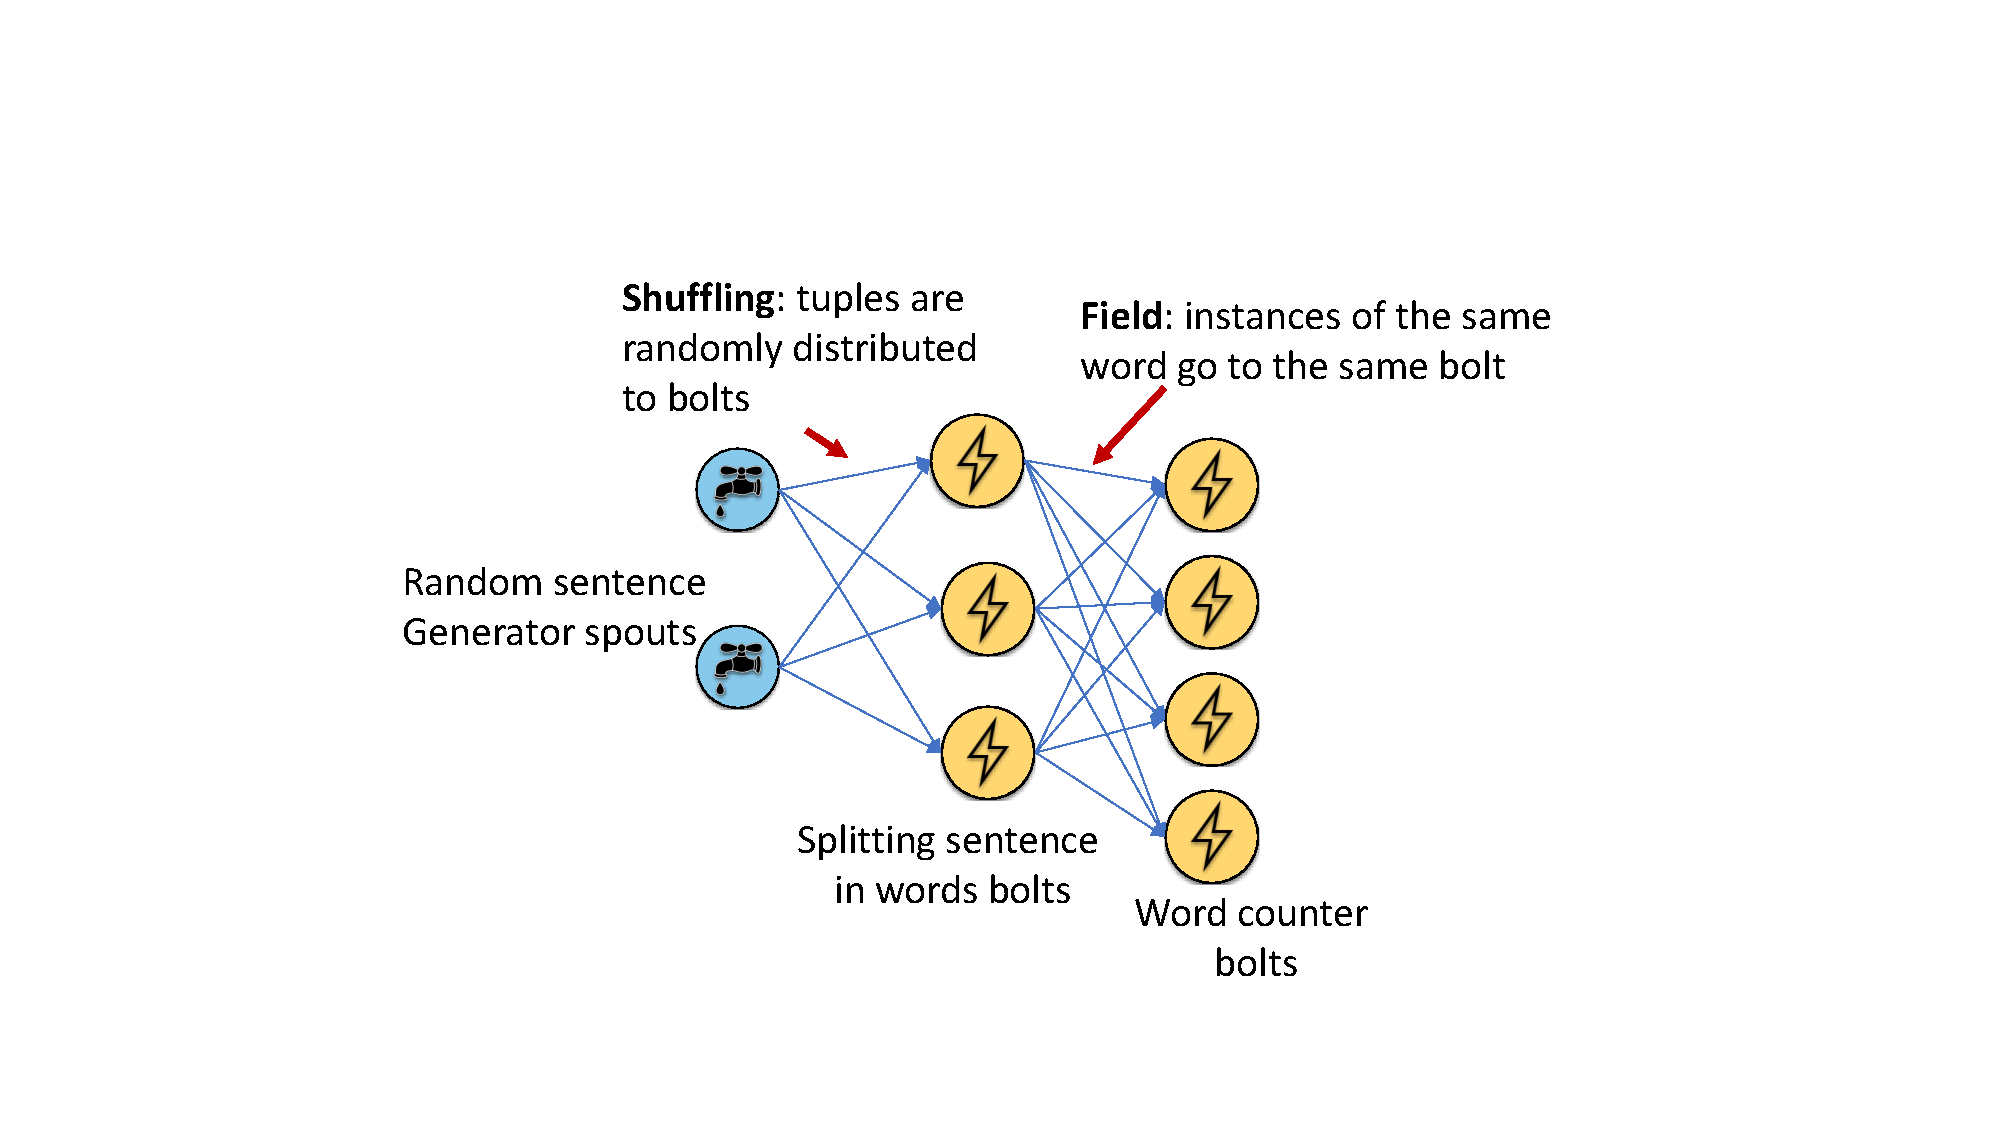
\includegraphics[width=\textwidth]{img/apache-storm.pdf}
    \end{center}
\end{examplebox}
    \subsubsection{Combining batch and stream: Lambda Architecture}

\definition{Lambda architecture} is a \textbf{data-processing architecture} designed to handle massive quantities of data by taking advantage of both batch and stream-processing methods. 

\highspace
This approach to architecture attempts to balance latency, throughput, and fault-tolerance by using batch processing to provide comprehensive and accurate views of batch data, while simultaneously using real-time stream processing to provide views of online data. The two view outputs may be joined before presentation. 

\highspace
The rise of lambda architecture is correlated with the growth of big data, real-time analytics, and the drive to mitigate the latencies of map-reduce.

\begin{figure}[!htp]
    \centering
    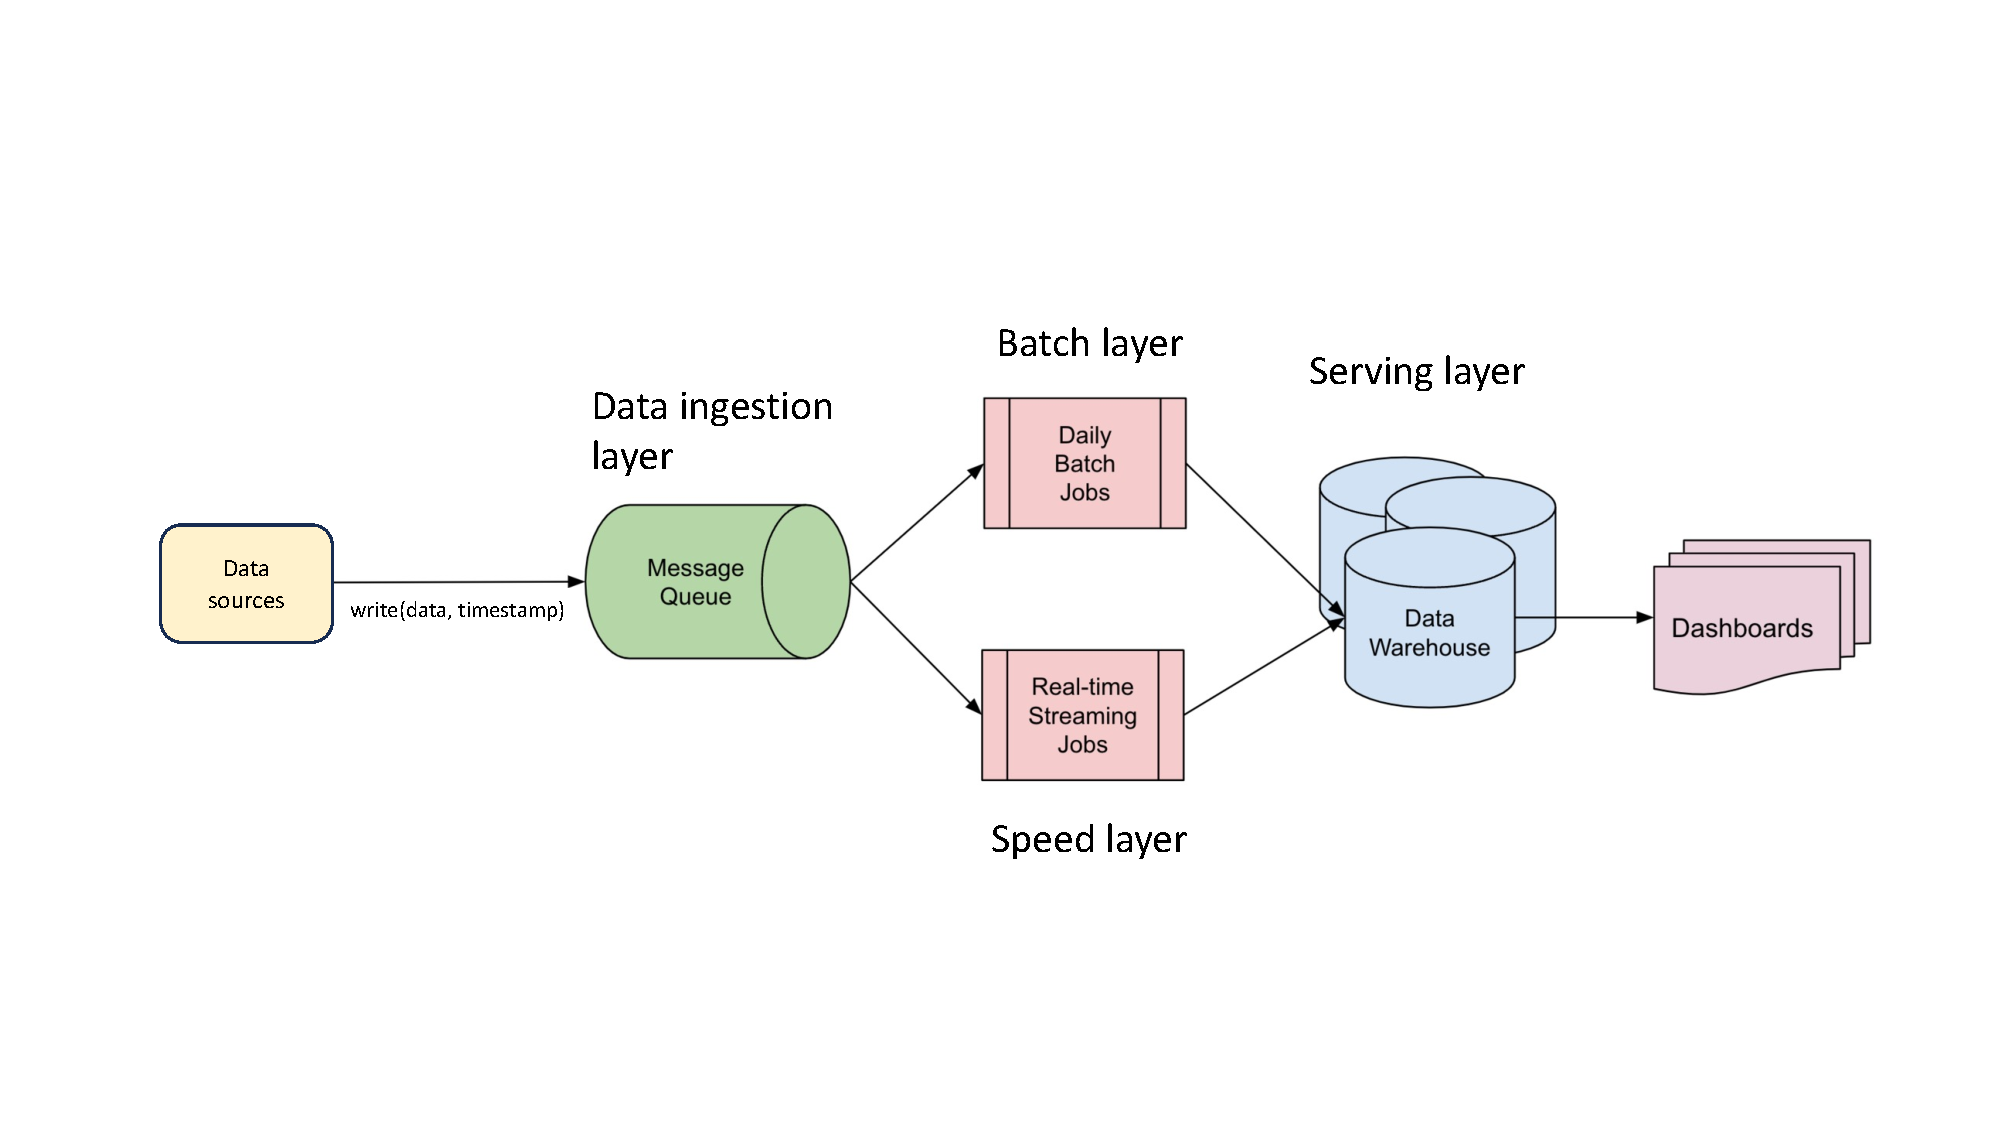
\includegraphics[width=\textwidth]{img/lambda-arch.pdf}
    \caption{Lambda architecture.}
\end{figure}

Exist also \definition{Kappa architecture}. Kappa architecture is a software architecture used for processing streaming data with a single technology stack. It is a simplification of Lambda architecture, where the data is processed in batches. Kappa architecture ingests data into a messaging system like Apache Kafka, and performs both real-time and batch processing, especially for analytics, on the same stream. It allows for recomputation on the data by streaming it through the pipeline again.

    %%%%%%%%%%%%%%%%%%%%%%%%%%%%%%%
    % Verification and Validation %
    %%%%%%%%%%%%%%%%%%%%%%%%%%%%%%%
    \section{Verification and Validation}

\subsection{Terminology}

There are some differences between the terms verification and validation.

\highspace
First of all, the verification is internal. Despite the validation is external. Assuming an abstract process with the following levels:

\begin{figure}[!htp]
    \centering
    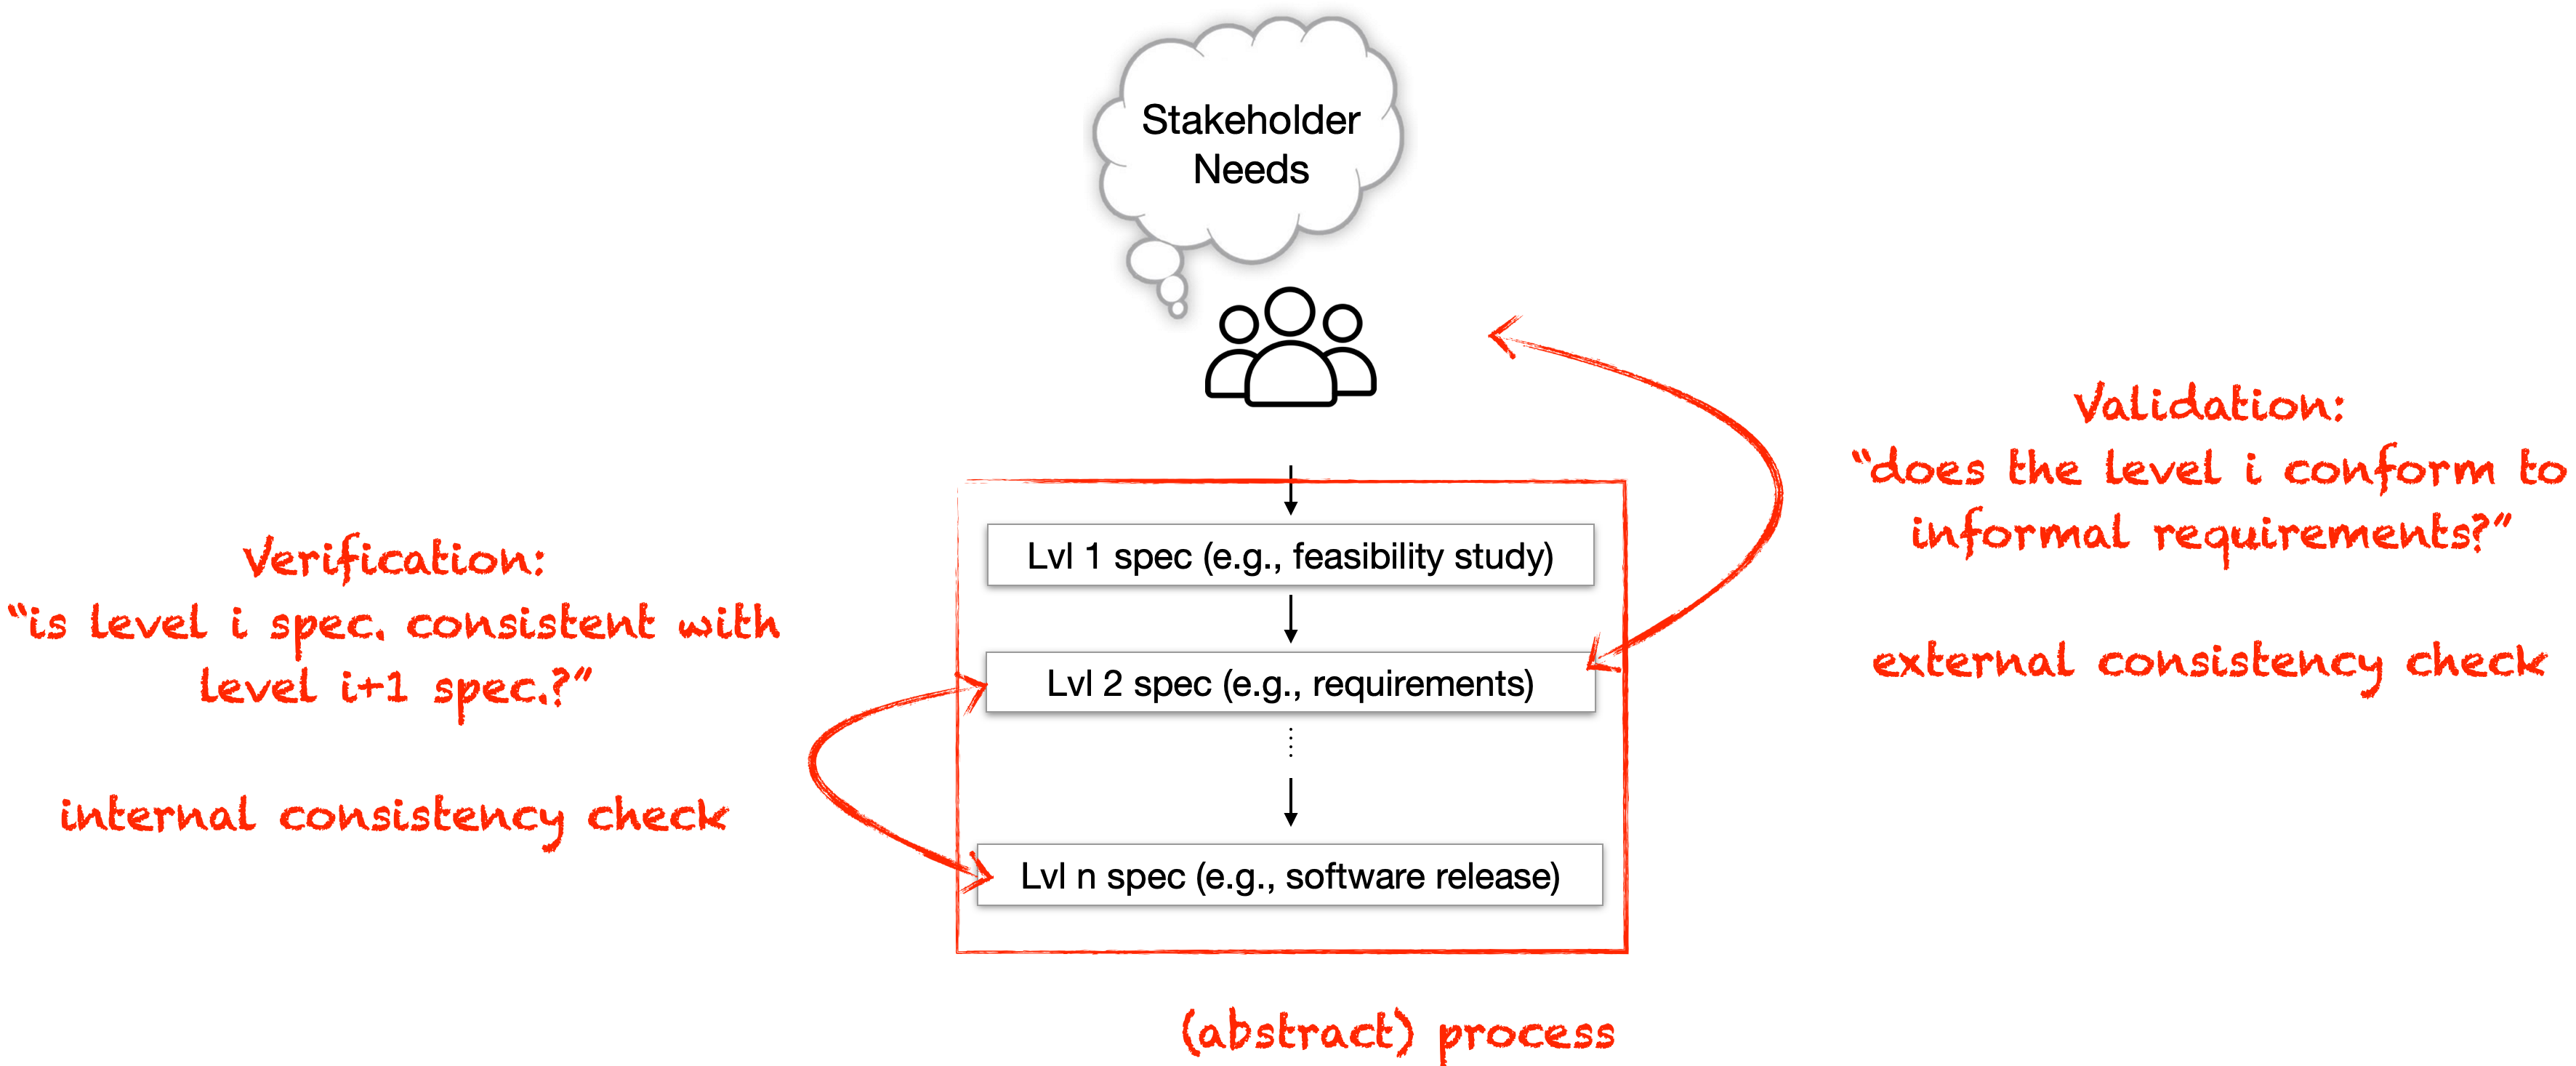
\includegraphics[width=\textwidth]{img/verification-and-validation-1.png}
\end{figure}

\noindent
The \textbf{verification} is intended as: \dquotes{Is level i consistent with level $i+1$?}. It's an \textbf{internal consistency check}. The \textbf{validation} is: \dquotes{Does level i conform to needs?}. It's an \textbf{external consistency check}.

\highspace
\href{https://en.wikipedia.org/wiki/A_Guide_to_the_Project_Management_Body_of_Knowledge}{The PMBOK guide}, also adopted by the \href{https://en.wikipedia.org/wiki/IEEE}{IEEE} as a standard, defines them as follows in its 4th edition:
\begin{itemize}
    \item \definition{Validation}. The assurance that a \textbf{product}, \textbf{service}, or \textbf{system} \textbf{meets the needs of the customer and other identified stakeholders}. It often involves acceptance and suitability with external customers. Contrast with verification.
    
    \item \definition{Verification}. The \textbf{evaluation of whether or not a product}, \textbf{service}, or \textbf{system complies with a regulation}, \textbf{requirement}, \textbf{specification}, or \textbf{imposed condition}. It is often an internal process. Contrast with validation.
\end{itemize}

\highspace
Another fundamental topic when we speak about verification and validation is \definition{Quality Assurance (QA)}. It \textbf{defines the policies and processes to achieve quality}. So it can \textbf{judge the quality and find defects}. 

A direct \textbf{consequence} of the QA is the \textbf{improvement of the quality}. With the term \dquotes{quality}, we refer to an ideal absence of defects (impossible) and an absence of other issues that prevent the fulfilment of non-functional requirements or the degradation of some software qualities.

\highspace
Since it is impossible to have zero defects, a \textbf{periodic quality assurance evaluation is critical}. Ideally, every artefact shall be the subject of QA; even the verification artefacts must be verified!

\newpage

\noindent
The \definition{V-model} is a \textbf{graphical representation of a systems development lifecycle}. It is used to produce rigorous development lifecycle models and project management models. It describes the activities and the results that must be made during product development.

\begin{figure}[!htp]
    \centering
    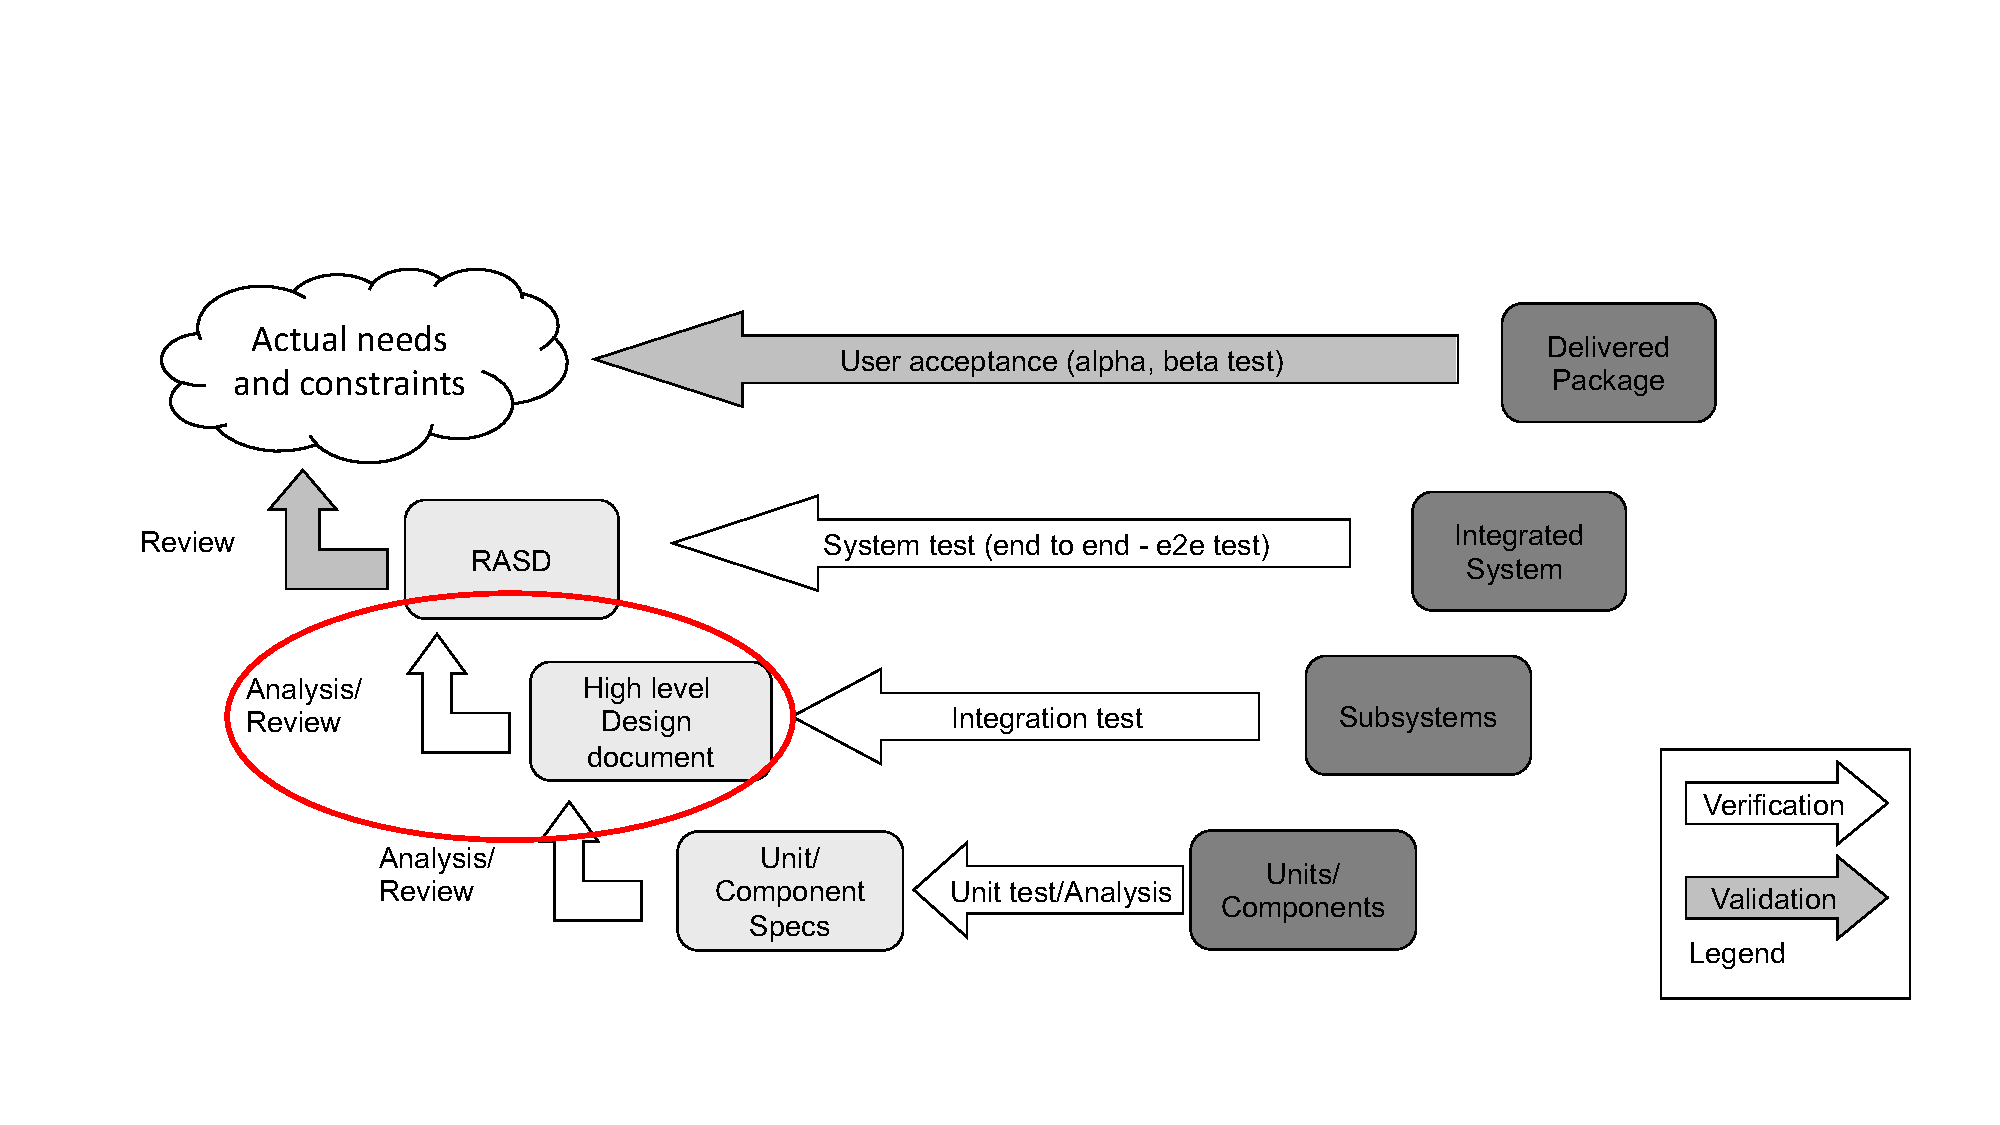
\includegraphics[width=\textwidth]{img/v-model-1.pdf}
    \caption{The V-model; verification is emphasized on the left.}
\end{figure}

\noindent
The \emph{left side} of the \dquotes{V} represents the decomposition of requirements and the creation of system specifications. The \emph{right side} of the \dquotes{V} represents an integration of parts and their validation.

\highspace
We have presented the V-model to help you understand where the verification can be placed.

\highspace
Now, the \textbf{verification} is concerned with the code and the architecture. Considering the \textbf{software} side, it has two possible approaches:
\begin{itemize}
    \item \definition{Static Analysis}. It is \textbf{done using source code or other software artefacts but \emph{without execution}}. Note that the analysis is static, but the properties are dynamic.

    \item \definition{Dynamic Analysis (Testing)}. It is \textbf{done by executing the sources}. The analysis is made by \textbf{comparing} the actual behaviour and the expected one.
\end{itemize}
On the other hand, to verify the \textbf{architectural level}, it is necessary to consider some aspects:
\begin{itemize}
    \item The \textbf{structure must be consistent}. Some \example{examples}:
    \begin{itemize}
        \item For every required interface, a corresponding provided interface exists.
        
        \item Sequence diagrams are consistent with component diagrams and with the defined interfaces.
        
        \item Each component has one or more modules that implement it.
    \end{itemize}

    \item All \textbf{functional requirements must have the possibility to be satisfied}. Some \example{examples}:
    \begin{itemize}
        \item Each requirement is mapped on one or more components.
        
        \item Each use case event flow is detailed in terms of one or more sequence diagrams.
    \end{itemize}

    \item \textbf{Concurrent use of resources must be correctly defined}. Problems like order violation or a deadlock are expected. Some techniques must be applied to analyze these problems. 
    
    \item \textbf{Non-functional requirements must have the possibility to be fulfilled}.
\end{itemize}
    \subsubsection{Study concurrent use of resources at architectural level (PT Net)}\label{subsubsection: study concurrent use of resources at architectural level (PT Net)}

It is necessary to model distributed systems to study the concurrent use of resources at the architectural level.

\highspace
A \definition{Petri Net (PT Net or P/T Net)}, a place/transition net (PT net), is one of several \textbf{mathematical modelling languages used to describe distributed systems}. Like industry standards such as UML activity diagrams, \textbf{Petri nets offer a graphical notation for stepwise processes} that include choice, iteration, and concurrent execution.

\highspace
The Petri net uses a graphic tool. It is a bipartite-directed graph containing places (circles), transitions (bars), and directed arcs.

\highspace
A Petri net is a four-tuple:
\begin{equation}
    PN = <P, T, I, O>
\end{equation}
\begin{itemize}
    \item $P$: a \textbf{finite set of places} $\left\{p_{1}, p_{2}, \dots, p_{n}\right\}$
    
    \item $T$: a \textbf{finite set of transitions} $\left\{t_{1}, t_{2}, \dots, t_{s}\right\}$
    
    \item $I$: an \textbf{input function} $\left(T \times P\right) \longrightarrow \left\{0,1\right\}$
    
    \item $O$: an \textbf{output function} $\left(T \times P\right) \longrightarrow \left\{0,1\right\}$
\end{itemize}
It's also possible to add another term called $M^{0}$, which is an \textbf{initial marking} $P \longrightarrow N$:
\begin{equation}
    PN = <P, T, I, O, M^{0}>
\end{equation}
Formula called also \textbf{marked Petri net}.

\highspace
You can find a detailed explanation \href{https://isr.umd.edu/Labs/CIM/miscs/wmsor97.pdf}{here}. Some observations of the Petri net:
\begin{itemize}
    \item In a given marking $M$, a transition $t$ can fire only if it is enabled.

    \item An enabled transition not necessarily fires.

    \item More than one transition can be enabled in a marking.

    \item If two transitions are enabled at the same time:
    \begin{itemize}
        \item Which one fires first is not determined;
        \item Petri nets are an intrinsically nondeterministic model;
        \item The firing of a transition might disabled another enabled transition.
    \end{itemize}
\end{itemize}
In fact, if two transitions are enabled at the same time, they can fire simultaneously unless the firing of one transition disables the other. Petri nets are \textbf{suitable for modelling concurrent systems}. On \href{http://petrinet.org/}{this page} you can see a live simulation by clicking on the nodes.

\newpage

\begin{figure}[!htp]
    \centering
    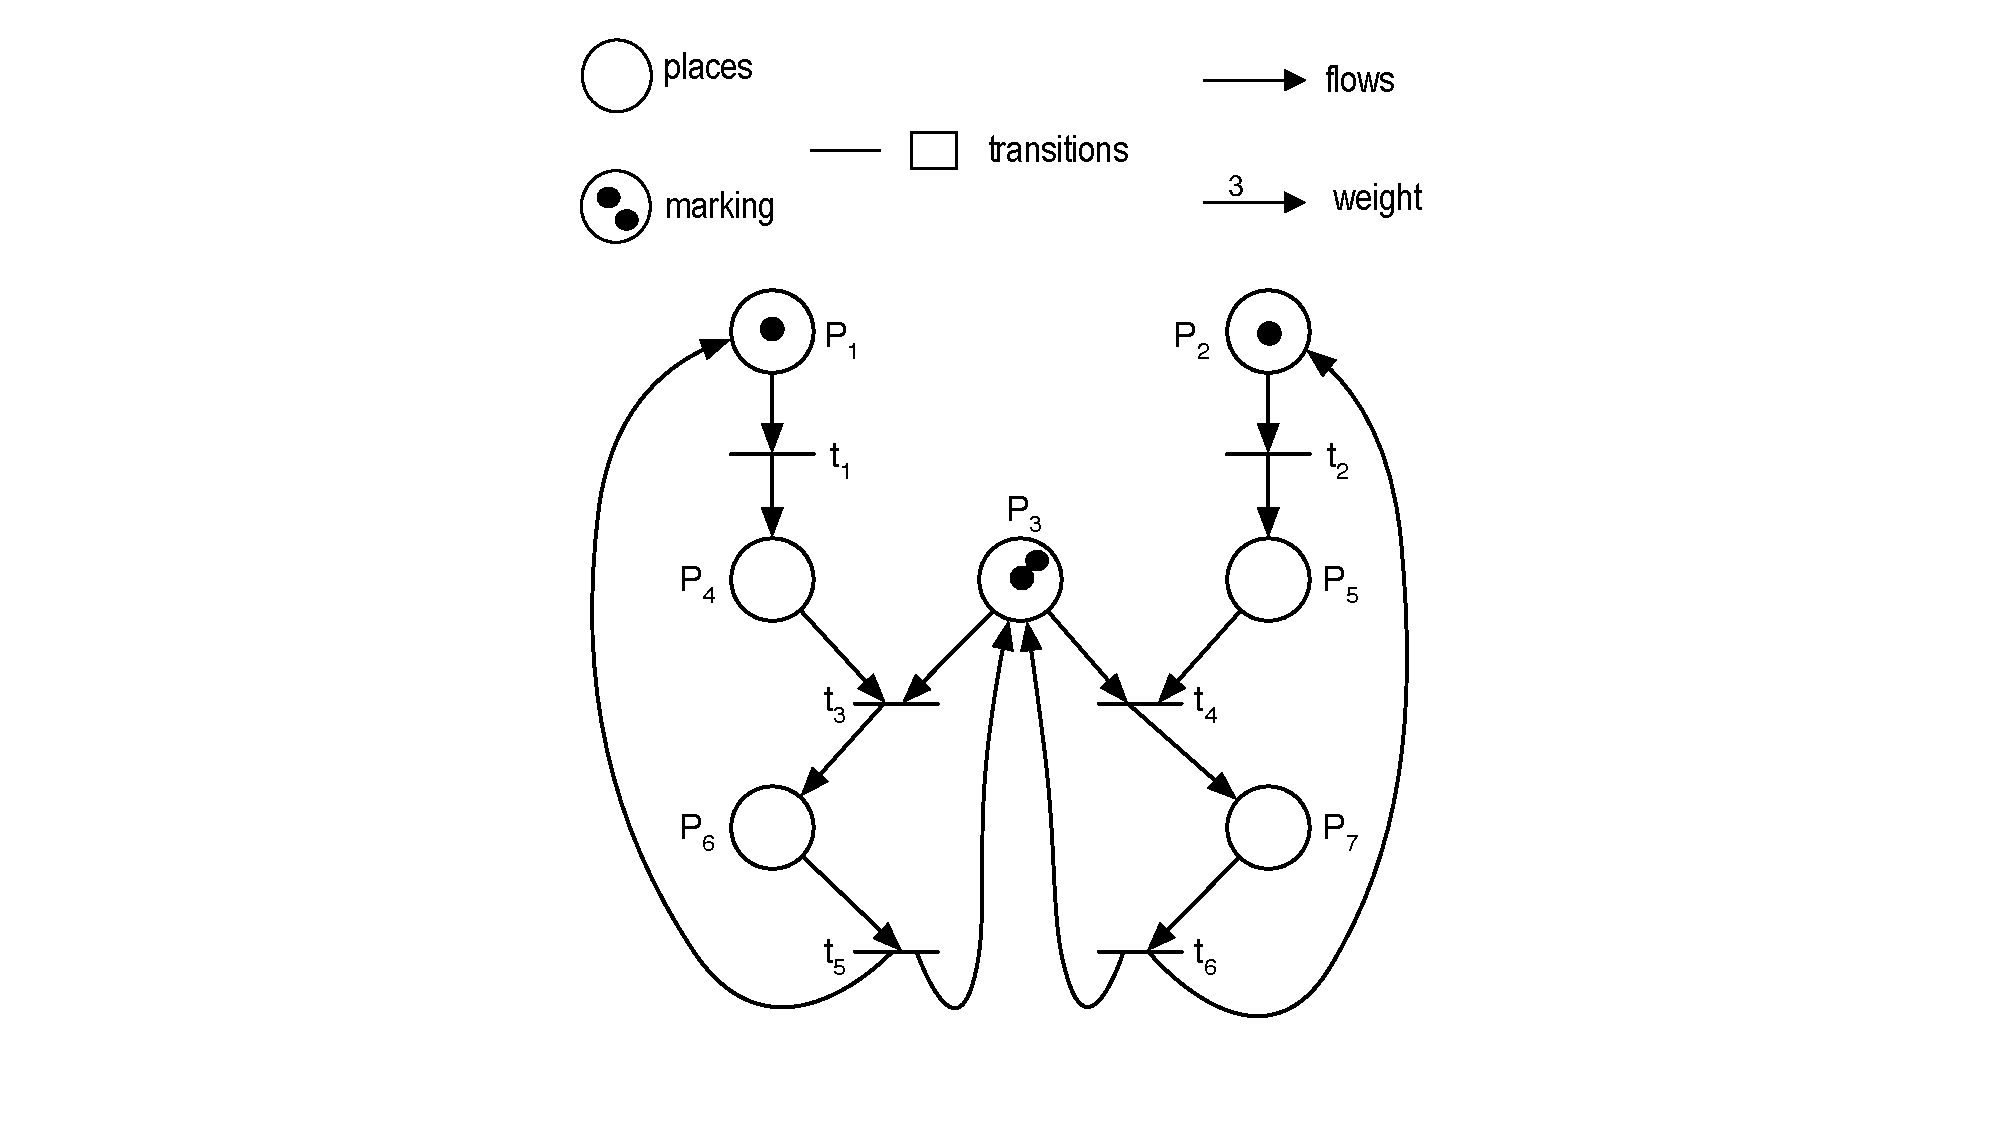
\includegraphics[width=.6\textwidth]{img/petri-nets-1.pdf}
    \caption{\example{Example} of Petri nets.}
\end{figure}

\begin{figure}[!htp]
    \centering
    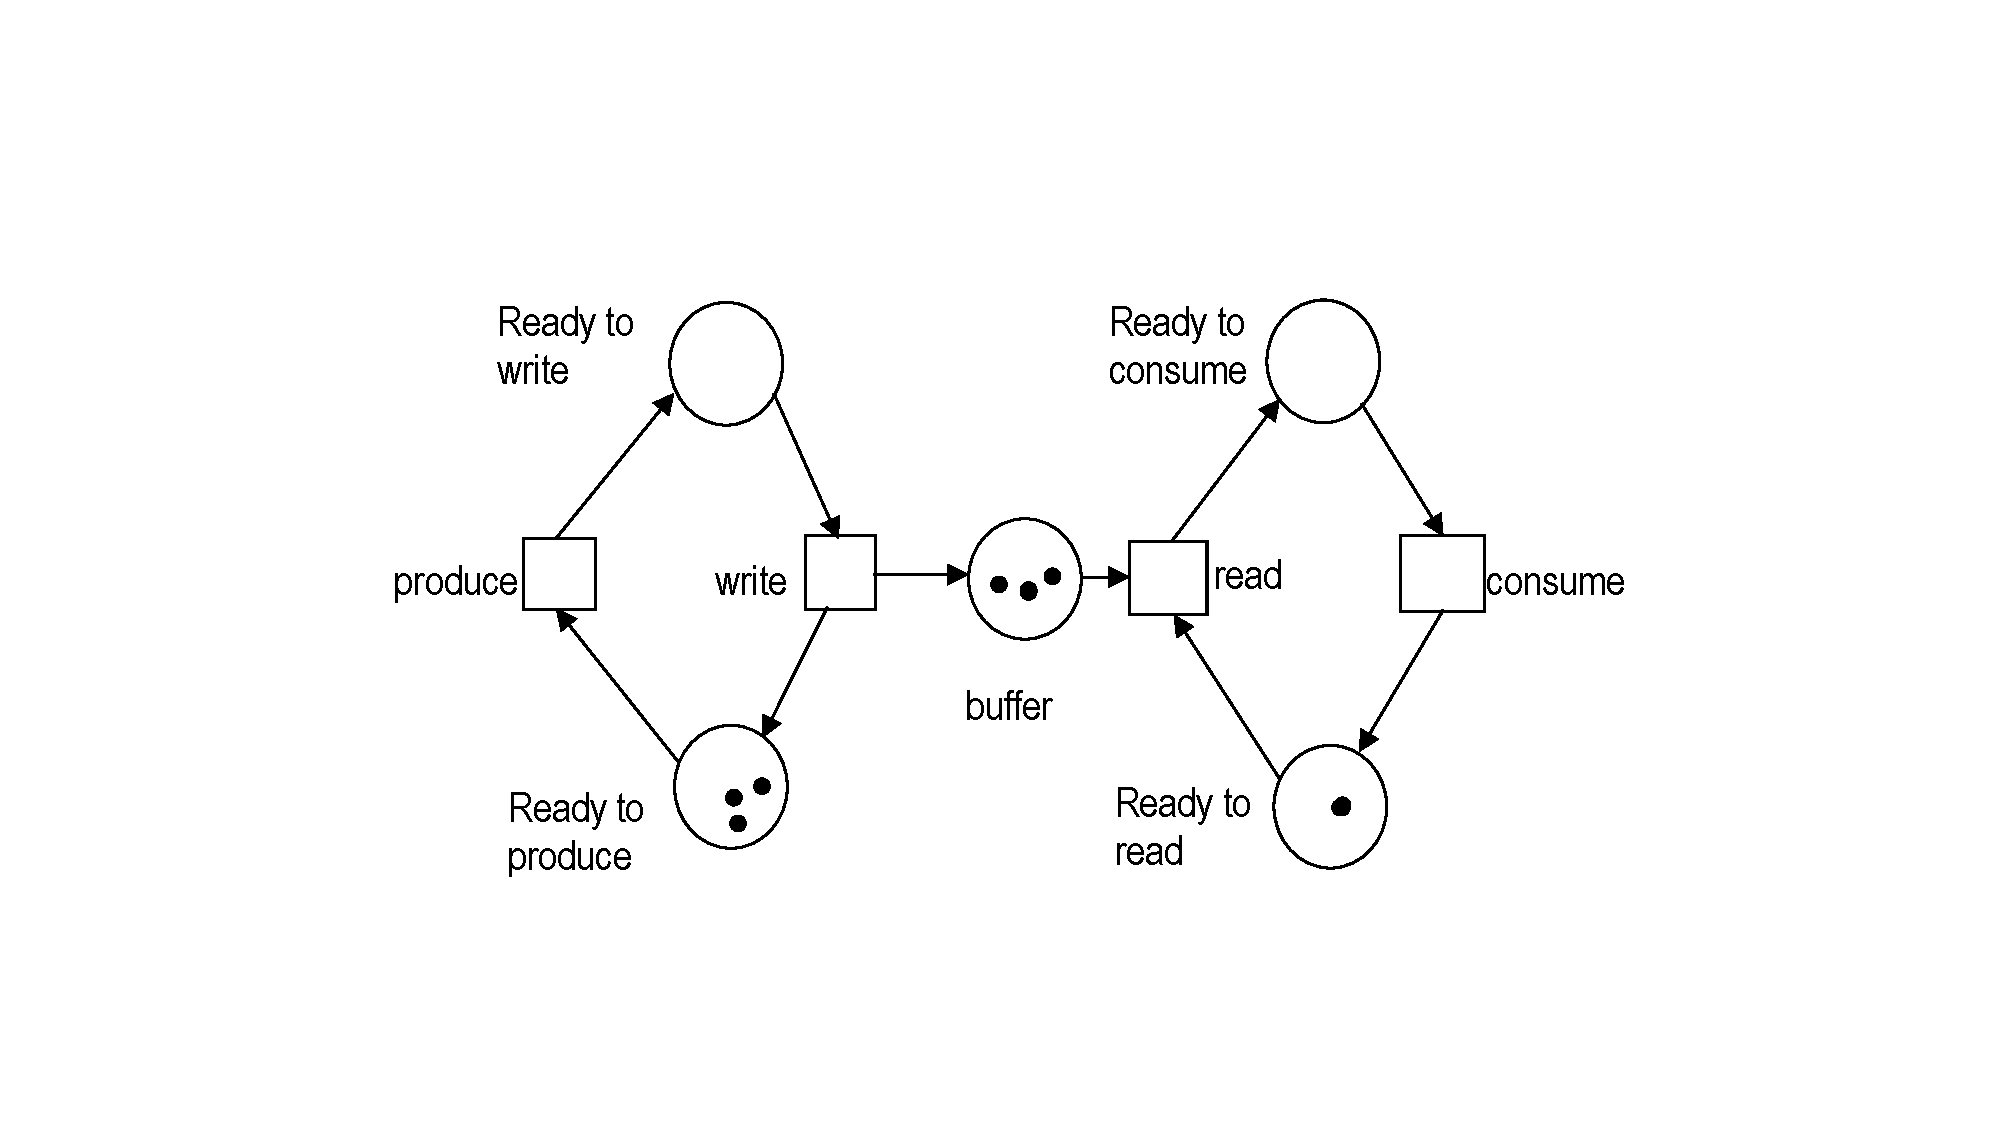
\includegraphics[width=.9\textwidth]{img/petri-nets-2.pdf}
    \caption{\example{Example} of Petri nets of producer-consumer model with unbounded buffer.}
\end{figure}

\newpage

\begin{figure}[!htp]
    \centering
    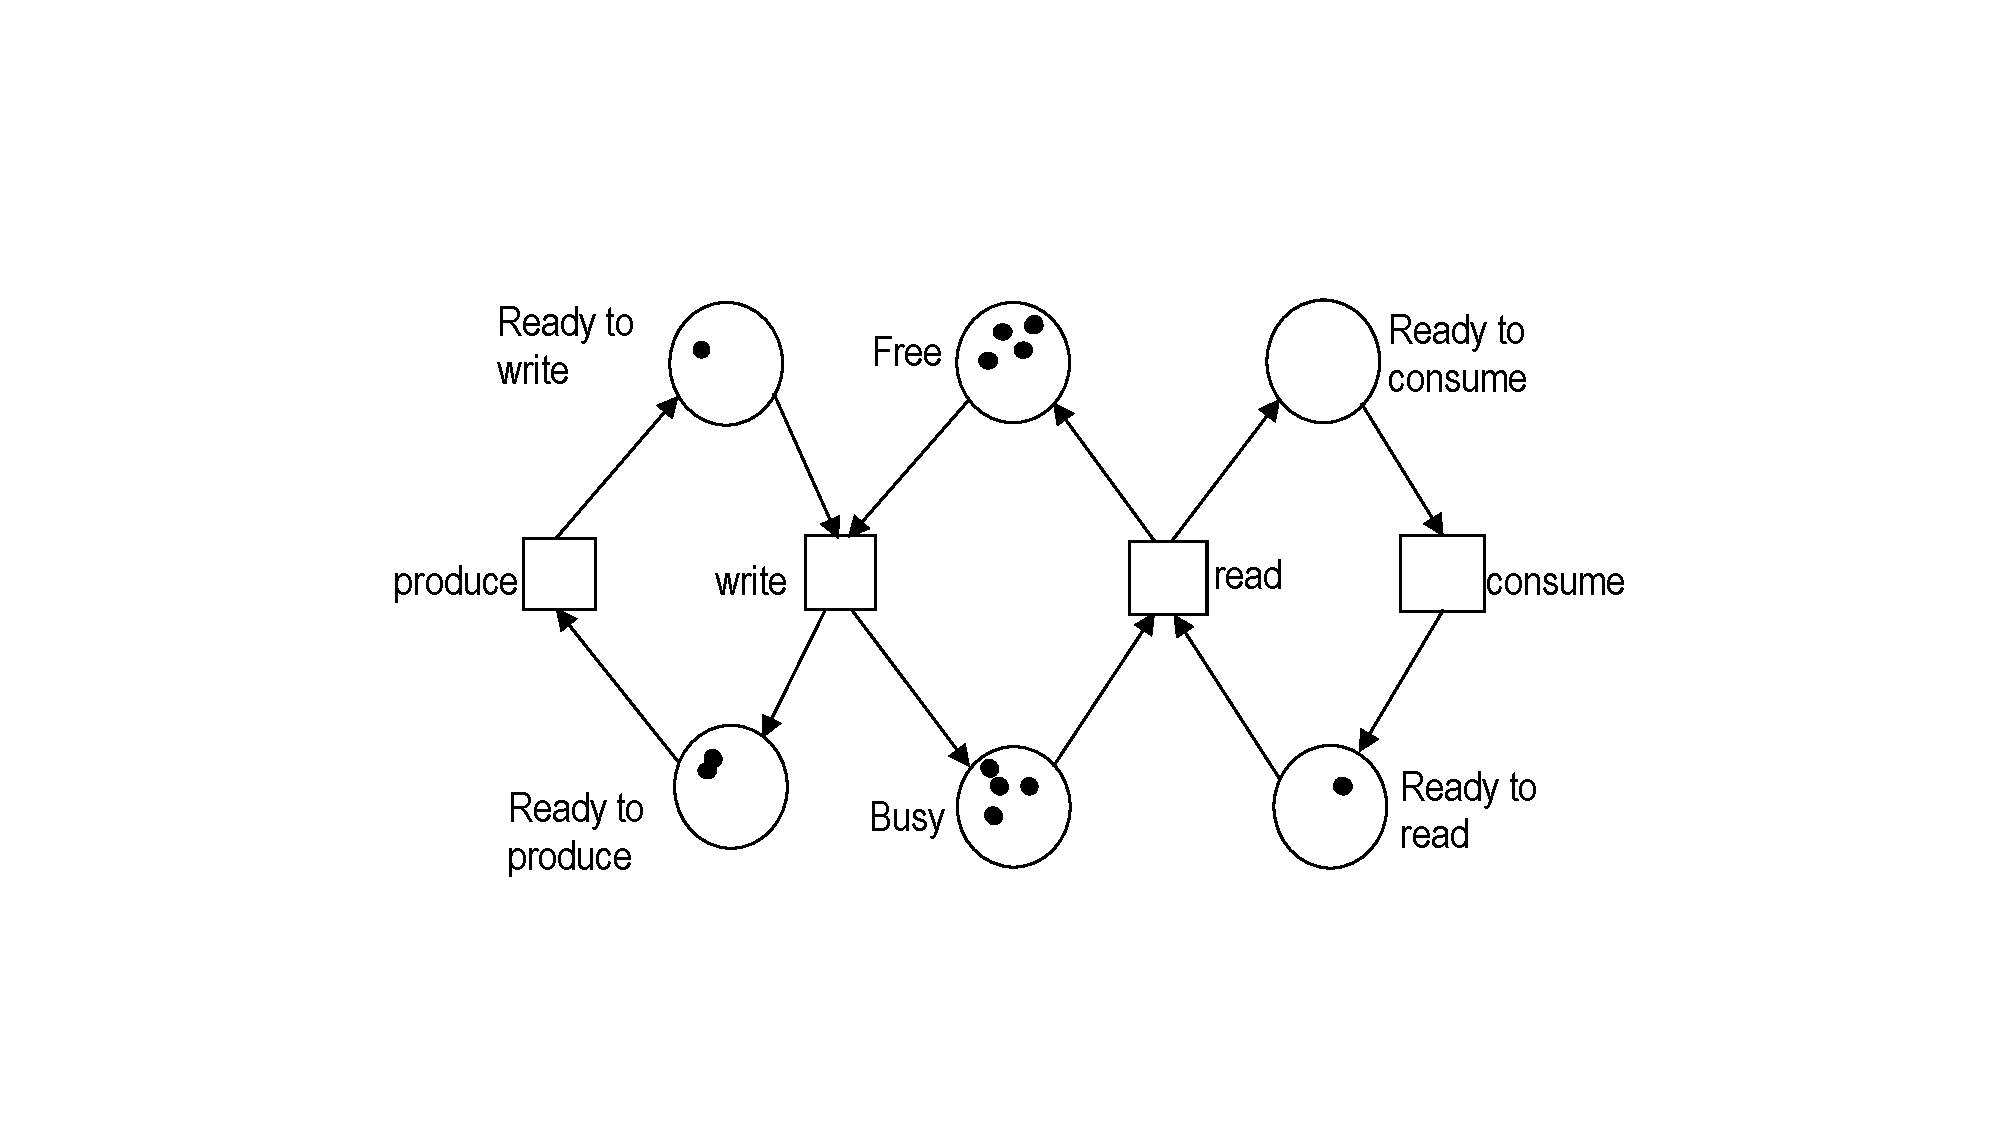
\includegraphics[width=.9\textwidth]{img/petri-nets-3.pdf}
    \caption{\example{Example} of Petri nets of producer-consumer model with finite buffer with a parametric number of positions.}
\end{figure}

\begin{figure}[!htp]
    \centering
    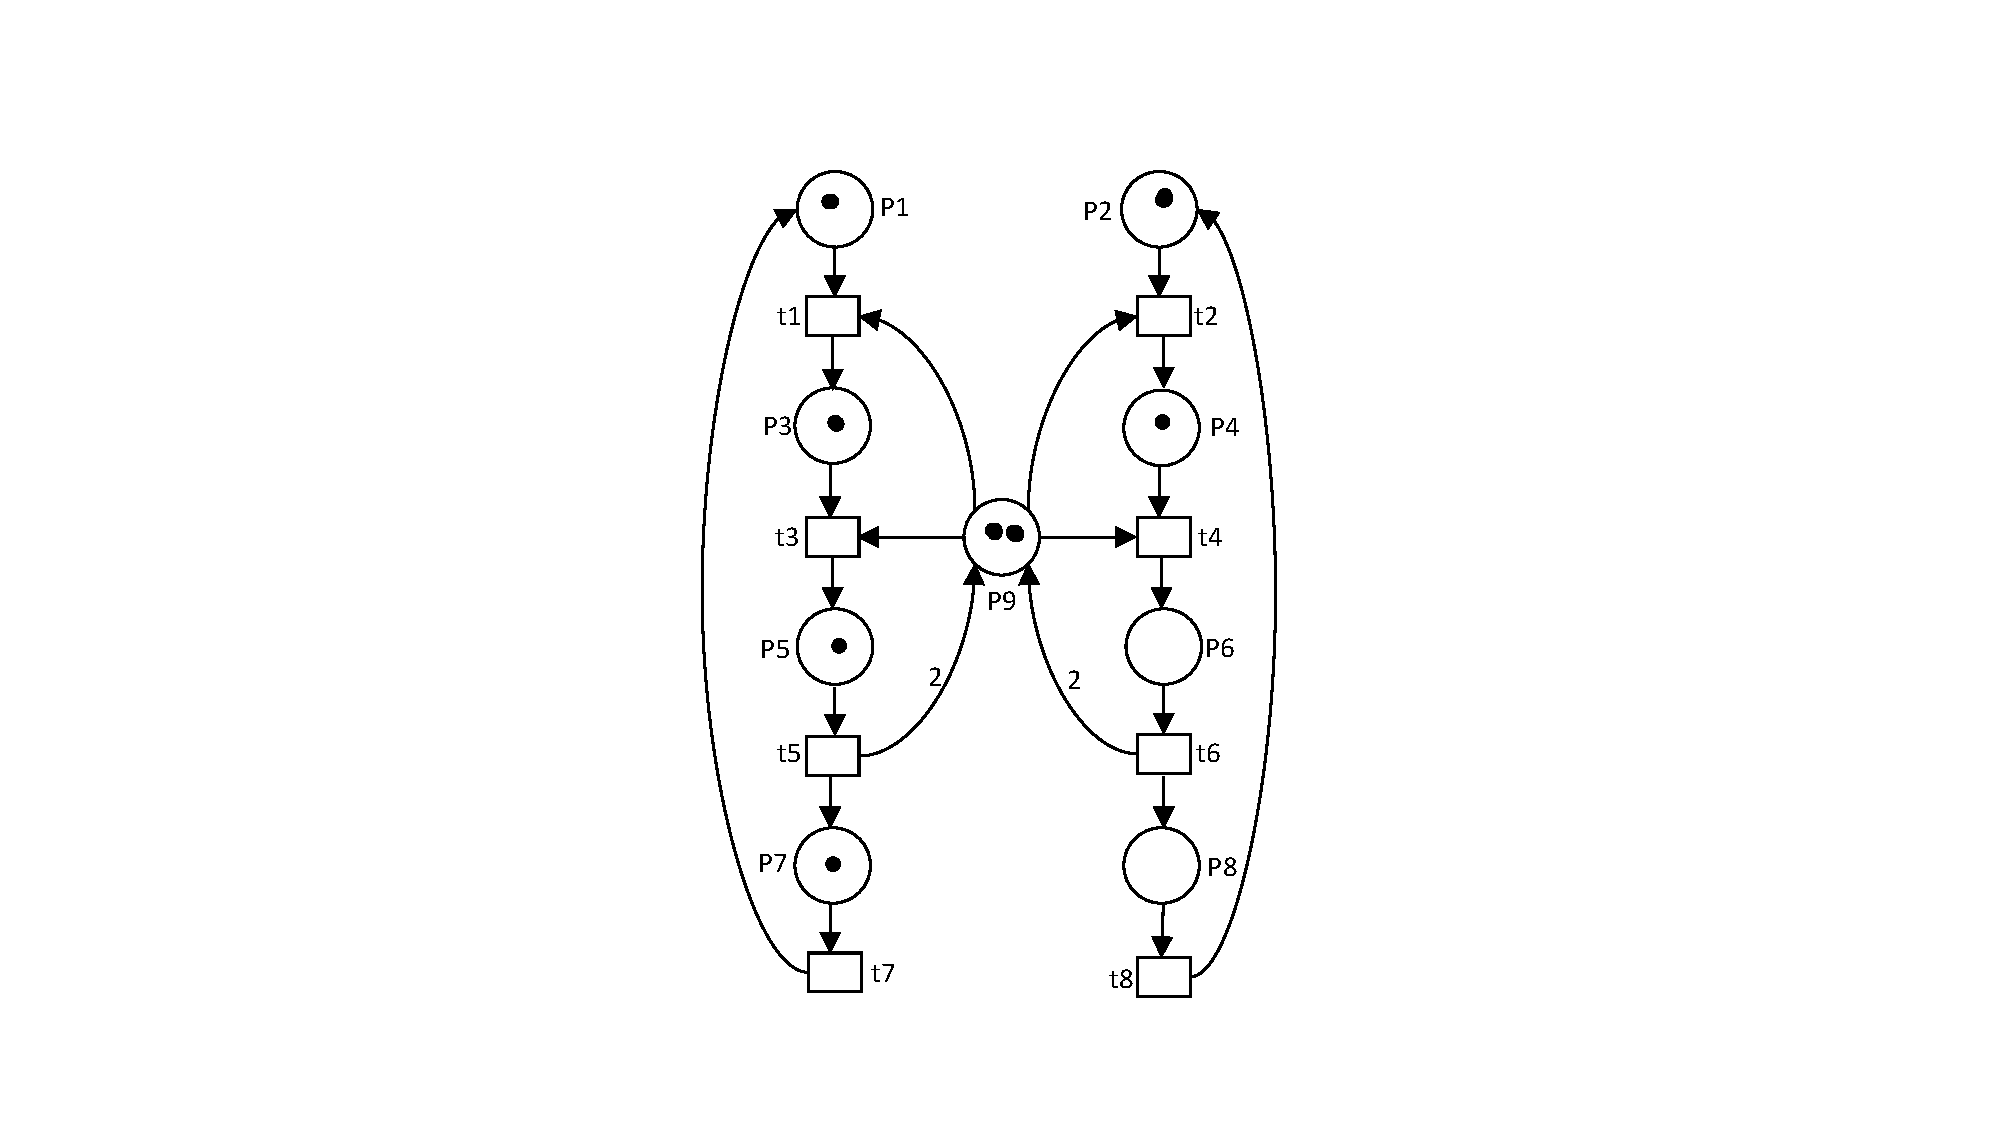
\includegraphics[width=.6\textwidth]{img/petri-nets-4.pdf}
    \caption{\example{Example} of Petri nets of deadlock.}
\end{figure}
    \subsubsection{Quantitative impact of architectural decisions}

Architectural choices directly influence several software qualities (e.g., scalability, reliability, availability, usability).

\highspace
To cope with this, we need metrics to quantify qualities and specific methodologies to analyze the quantitative impact of architectural choices on these qualities. The tactics are also foundational to address the issues.

\highspace
First, before discussing \emph{how to evaluate the quantitative impact of architectural decisions}, we must introduce the availability concept and explain a system life-cycle to introduce some exciting metrics.

\begin{flushleft}
    \textcolor{Green3}{\faIcon{question-circle} \textbf{Why is availability so important?}}
\end{flushleft}
In general, a \textbf{service shall be continuously available} to the user, and if it fails after a bit of downtime, it should be a \textbf{rapid service recovery}. So the \definition{availability} of a service depends on:
\begin{itemize}
    \item The \textbf{complexity} of the \textbf{infrastructure} architecture.
    
    \item \textbf{Reliability} of the individual components.
    
    \item \textbf{Ability to respond} quickly and effectively to faults.

    \item \textbf{Quality of the maintenance} by support organizations and suppliers.

    \item \textbf{Quality} and scope of the \textbf{operational management} processes.
\end{itemize}

\begin{flushleft}
    \textcolor{Green3}{\faIcon{book} \textbf{Study the System Life-Cycle to use availability metrics}}
\end{flushleft}
The \definition{System Life-Cycle} relates to failures in the following way:

\begin{figure}[!htp]
    \centering
    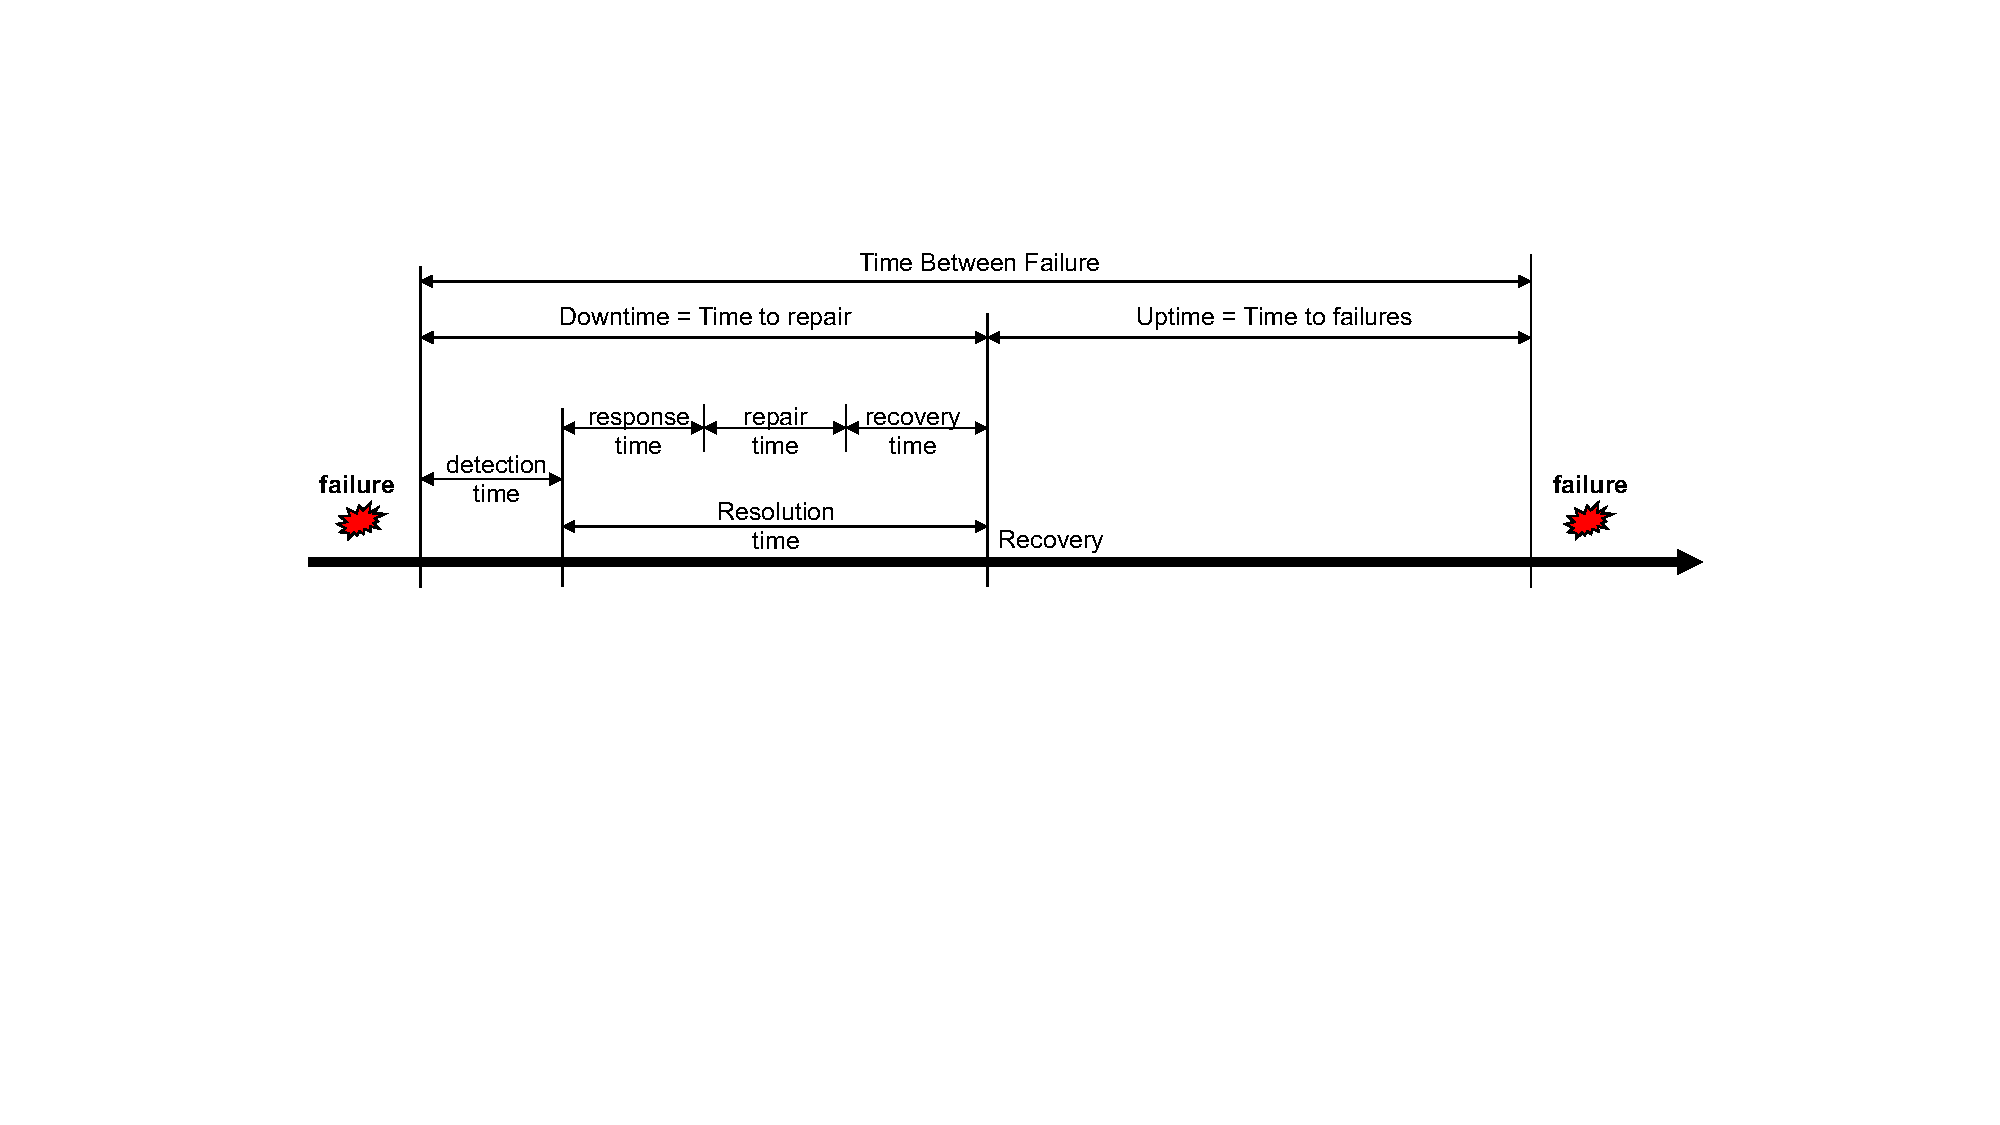
\includegraphics[width=\textwidth]{img/system-life-cycle-1.pdf}
    \caption{The System Life-Cycle when faults occur.}
    \label{fig: The System Life-Cycle when faults occur}
\end{figure}
\begin{itemize}
    \item \textbf{Time of occurrence}. Time at which the \emph{user} becomes aware of the failure.
    
    \item \textbf{Detection time}. Time at which \emph{operators} become aware of the failure.
    
    \item \textbf{Response time}. Time required by \emph{operators} to diagnose the issue and respond to users.
    
    \item \textbf{Repair time}. Time required to fix the service/components that caused the failure.
    
    \item \textbf{Recovery time}. Time required to restore the system (re-configuration, re-initialization, ...).
    
    \item \definition{Mean Time to Repair (MTTR)}. Average time between the occurrence of a failure and service recovery, also known as the \emph{downtime}.

    \item \definition{Mean Time to Failures (MTTF)}. Mean time between the recovery from one failure and the occurrence of the next failure, also known as \emph{uptime}.

    \item \definition{Mean Time Between Failures (MTBF)}. Mean time between the occurrences of two consecutive failures.
\end{itemize}

\begin{definitionbox}[: Availability Metric]
    The \definition{availability metric} is the \textbf{probability} that a \textbf{component} \textbf{works correctly} at \textbf{time} $t$. As a mathematician term, we can express this definition as the relationship between the Mean Time to Failures (MTTF) and the MTTF plus the Mean Time to Repair (MTTR):
    \begin{equation}\label{eq: availability metric}
        A = \dfrac{
            \texttt{MTTF}
        }{
            \texttt{MTTF} + \texttt{MTTR}
        }
    \end{equation}
\end{definitionbox}

\noindent
Note that if the Mean Time to Repair (MTTR) is small, then the Mean Time Between Failures (MTBF) is approximately equal to the Mean Time to Failures (MTTF): $\texttt{MTBF} \approxeq \texttt{MTTF}$.

\begin{flushleft}
    \textcolor{Green3}{\faIcon{question-circle} \textbf{Does an easier notation than the availability metric work?}}
\end{flushleft}
The availability metric is crucial for understanding how a component works at a particular time, but sometimes, we need an easier notation to represent availability. In these cases, we use the \definition{nines notation}.

\highspace
\textbf{Nines} are an informal logarithmic notation for proportions very near to one or, equivalently, percentages very near 100\%. Nines are the number of consecutive nines in a percentage such as 99\% (two nines). The number of nines of a proportion $x$ is:
\begin{equation}\label{eq: nines}
    \texttt{nines} = - \log_{10} \left(1-x\right)
\end{equation}
In the computer system availability (our context), a \emph{one nine} (90\%) uptime indicates a system that is available 90\% of the time or, more commonly described, unavailable 10\% of the time.
\begin{table}[!htp]
    \centering
    \begin{tabular}{@{} l l @{}}
        \toprule
        \textbf{Availability} & \textbf{Downtime} \\
        \toprule
        90\% (1-nine)       & 36.5 days/year \\
        99\% (2-nines)      & 3.65 days/year \\
        99.9\% (3-nines)    & 8.76 hours/year \\
        99.99\% (4-nines)   & 52 minutes/year \\
        99.999\% (5-nines)  & 5 minutes/year \\
        \bottomrule
    \end{tabular}
    \caption{Some nines notation and downtime values.}
\end{table}

\newpage

\begin{flushleft}
    \textcolor{Green3}{\faIcon{question-circle} \textbf{Now that we have the theory and the tools, what methodology should we use to analyze the impact of the architectural choices?}}
\end{flushleft}
The \definition{Analysis Methodology} depends on the system. The Availability is calculated by \textbf{modelling the system} as an interconnection of elements in series and parallel:
\begin{itemize}
    \item \textbf{Elements operating in \underline{series}} mean that if one element fails, the whole combination fails.
    
    \item \textbf{Elements operating in \underline{parallel}} mean that if a component fails, the other elements take over the operations of the failed element.
\end{itemize}

\begin{flushleft}
    \textcolor{Red2}{\faIcon{bookmark} \textbf{Availability in series}}
\end{flushleft}
The combined system is \textbf{operational only if every part is available}. Then, the combined Availability is the \textbf{product of the parts' Availability}.
\begin{equation}\label{eq: availability in series}
    A = \displaystyle\prod_{i=1}^{n} A_{i}
\end{equation}
\begin{examplebox}
    We assume there is a system composed of two components with the following availability and downtime:
    \begin{itemize}
        \item Component 1 has 99\% (2-nines) of availability and 3.65 days/year of downtime.
        \item Component 2 has 99.999\% (5-nines) of availability and 5 minutes/year of downtime.
    \end{itemize}
    So the combined availability is 98.999\% with 3.65 days/year of downtime. 
\end{examplebox}

\noindent
The downtime is calculated using the following formula:
\begin{equation*}
    \texttt{Downtime} = \left(1-A\right) \times 365 \:\texttt{days}/\texttt{year}
\end{equation*}
Note that the $A$ value is the Availability in terms of simple values and not as percentages (99\% become 0.99).

\highspace
In the previous example, we can see how the low Availability of Component 1 negatively affects the Availability of the entire system. This result means that a \textbf{chain is as strong as the weakest link}.

\newpage

\begin{flushleft}
    \textcolor{Red2}{\faIcon{bookmark} \textbf{Availability in parallel}}
\end{flushleft}
The combined system is \textbf{operational if at least one part is available}. Then, the combined Availability is $1-P$, where $P$ indicates all parts that are not available.
\begin{equation}\label{eq: availability in parallel}
    A = 1 - \displaystyle\prod_{i=1}^{n}\left(1-A_{i}\right)
\end{equation}

\begin{examplebox}
    We assume there is a system composed by two components with the following Availability and downtime:
    \begin{itemize}
        \item Component 1 has 99\% (2-nines) of Availability and 3.65 days/year of downtime.
        \item Component 2 has 99\% (2-nines) of Availability and 3.65 days/year of downtime.
    \end{itemize}
    Despite the previous example, the combined availability is 99.99\% (4-nines) with 52 minutes/year of downtime.
\end{examplebox}

\noindent
Even though components with very low Availability are used, the system's overall Availability is much higher than the Availability in series!

\begin{examplebox}
    Some examples of complex systems:
    \begin{itemize}
        \item $A_{7} = 1 - \left(1-A_{1}\right)\left(1-A_{2}\right)$
        \begin{center}
            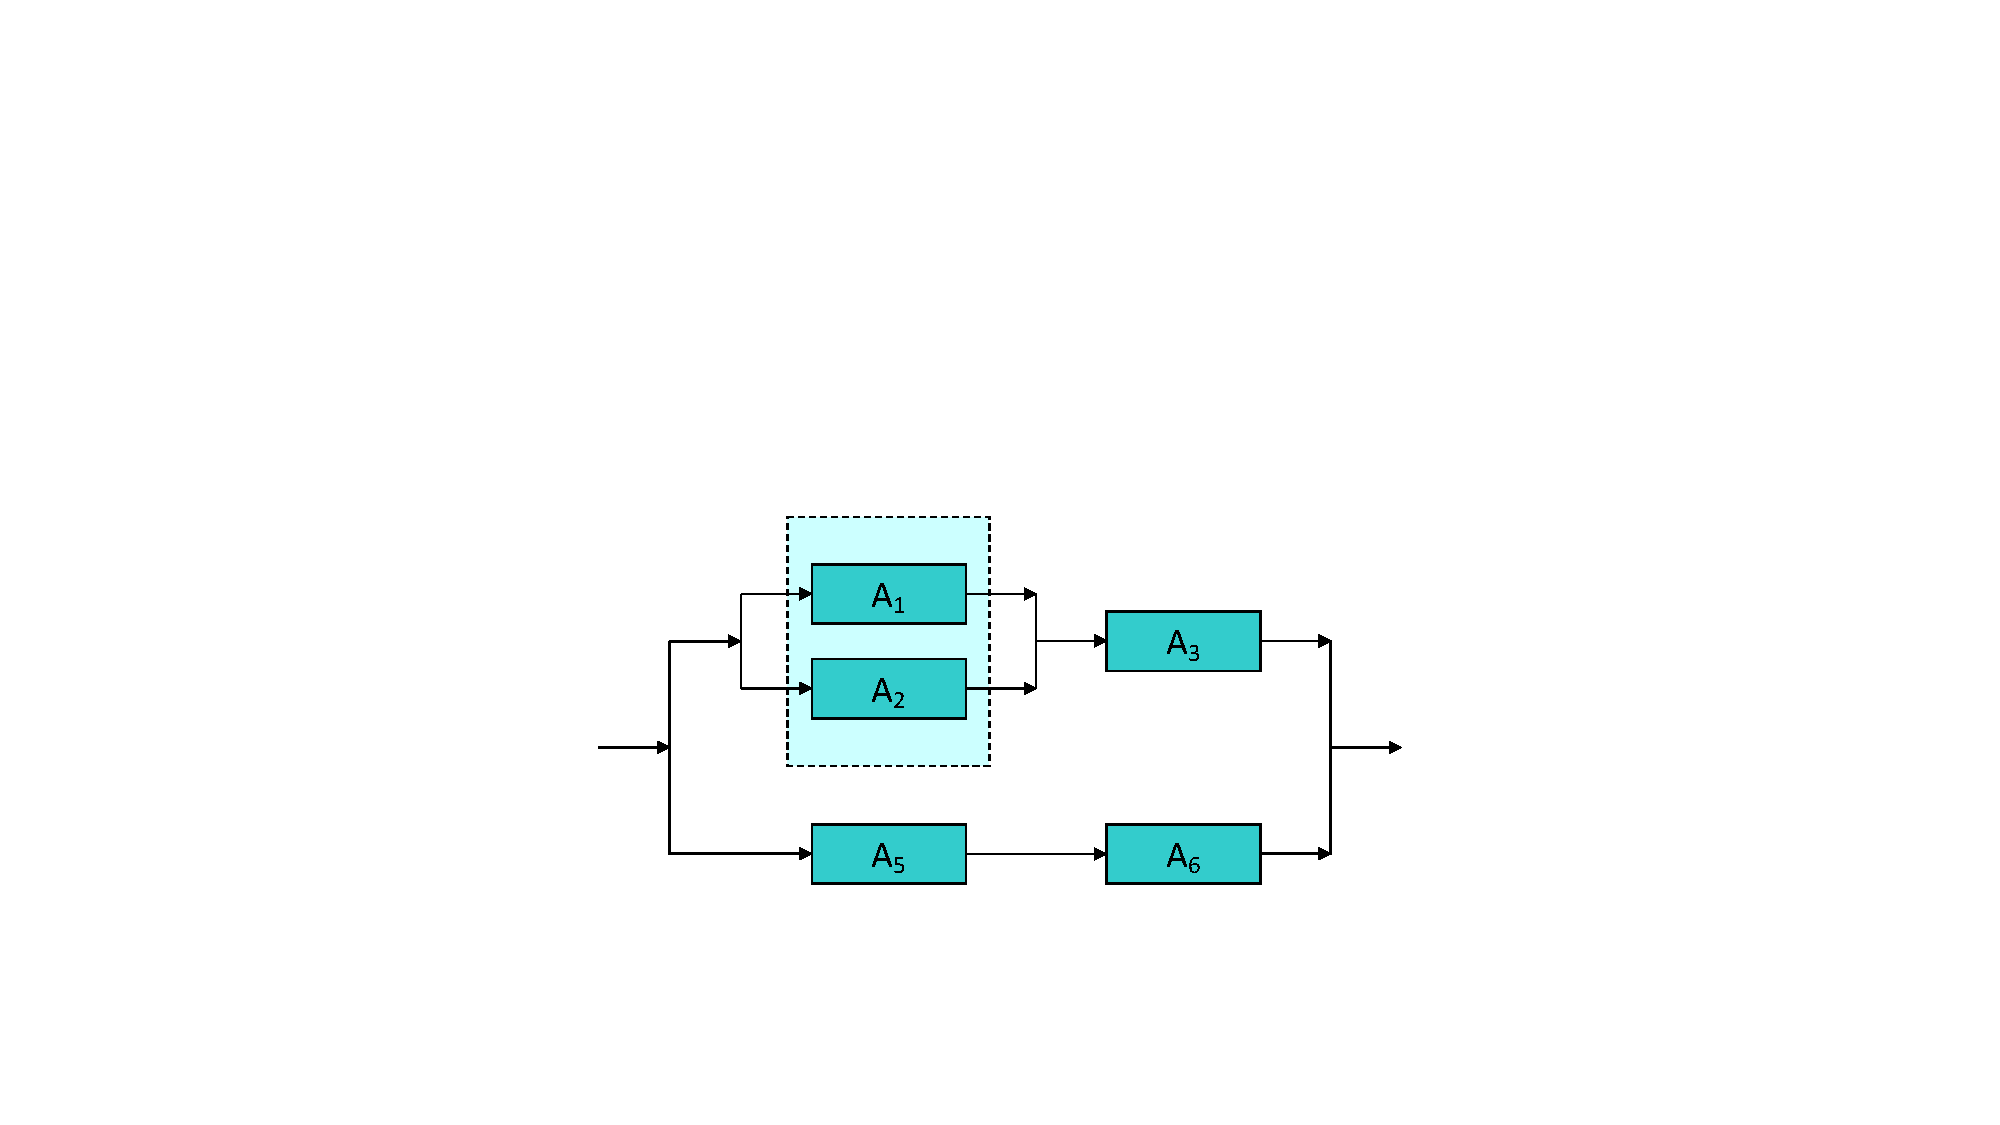
\includegraphics[width=.8\textwidth]{img/availability-in-parallel-1.pdf}
        \end{center}

        \item $A_{8} = A_{7}A_{3}$
        \begin{center}
            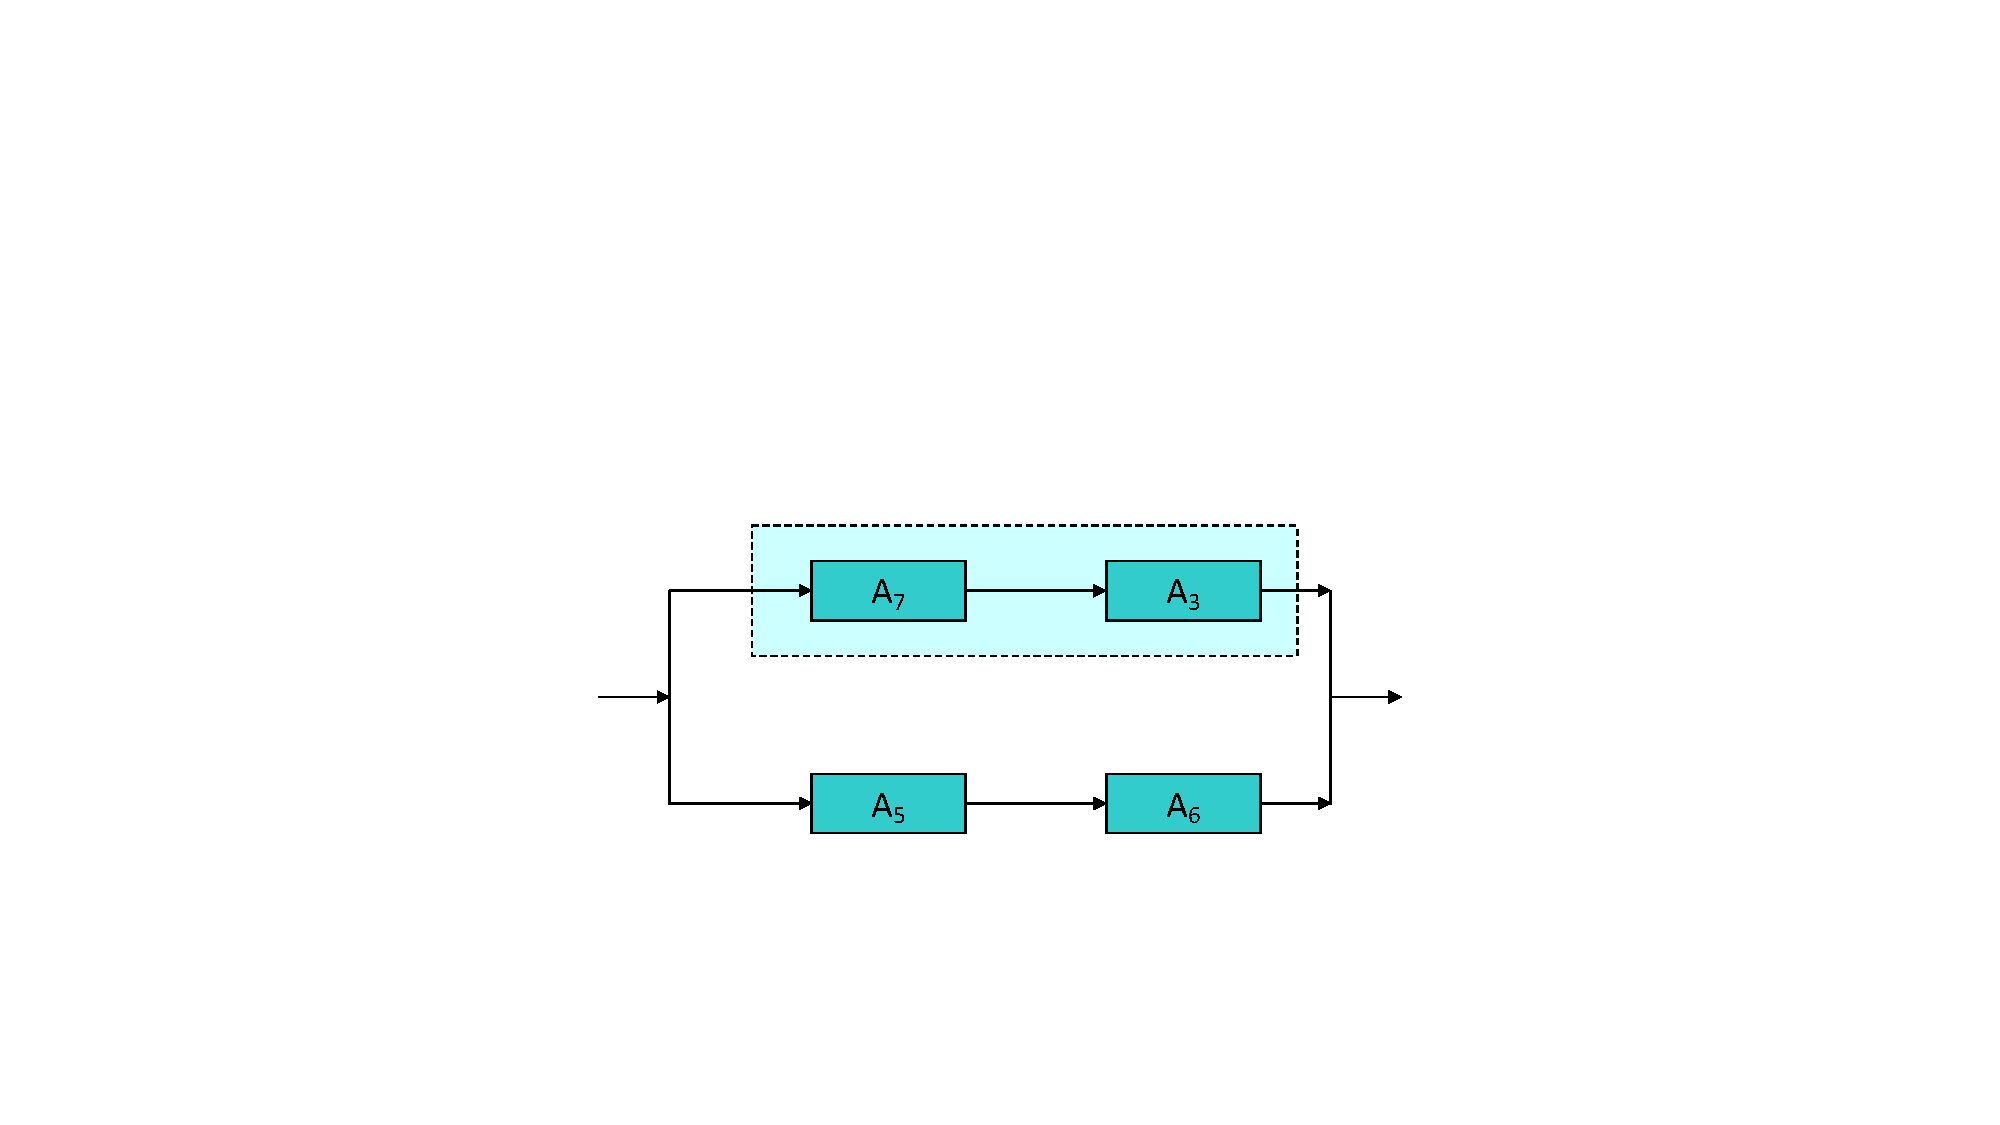
\includegraphics[width=.8\textwidth]{img/availability-in-parallel-2.pdf}
        \end{center}

        \item $A_{9} = A_{5}A_{6}$
        \begin{center}
            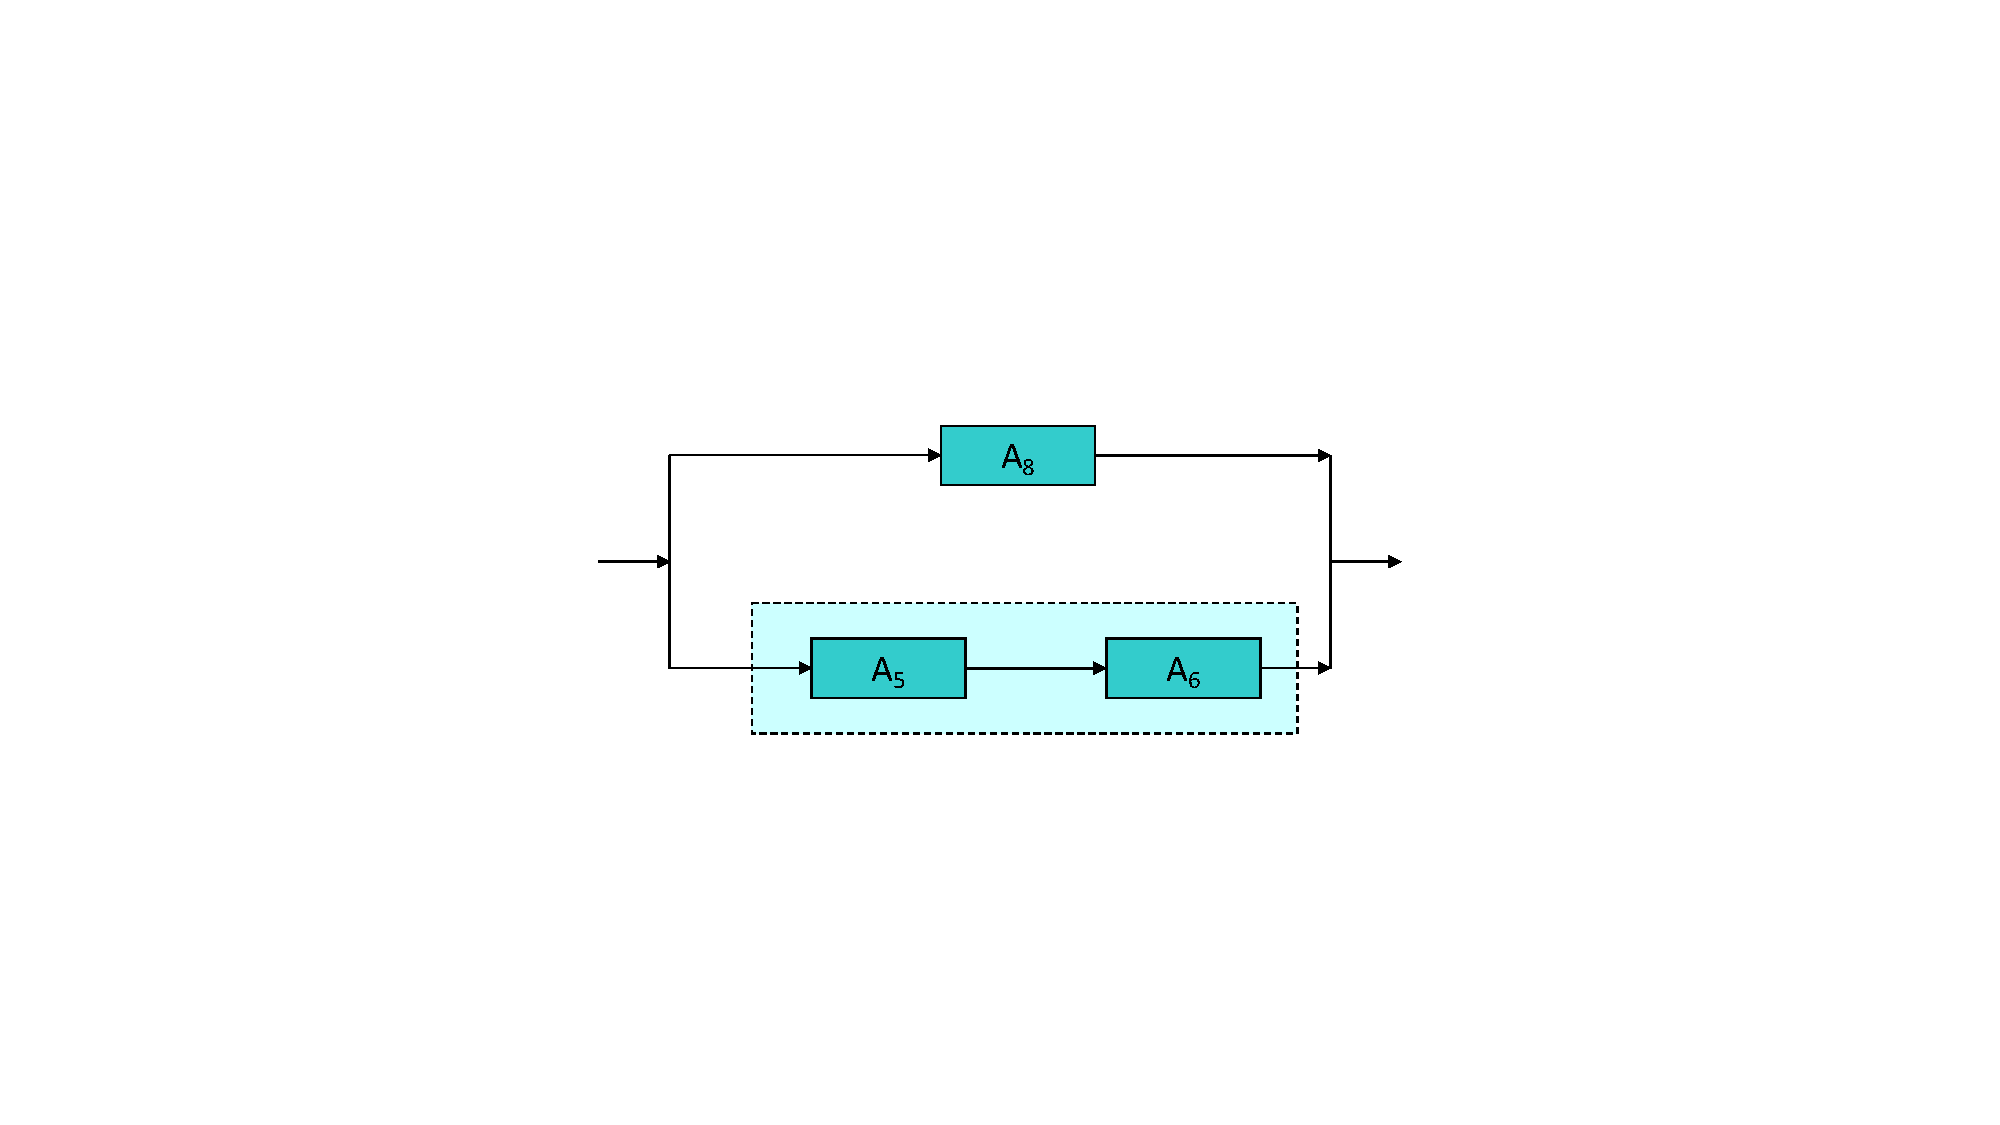
\includegraphics[width=.8\textwidth]{img/availability-in-parallel-3.pdf}
        \end{center}
        
        \item $A = 1 - \left(1-A_{8}\right)\left(1-A_{9}\right)$
        \begin{center}
            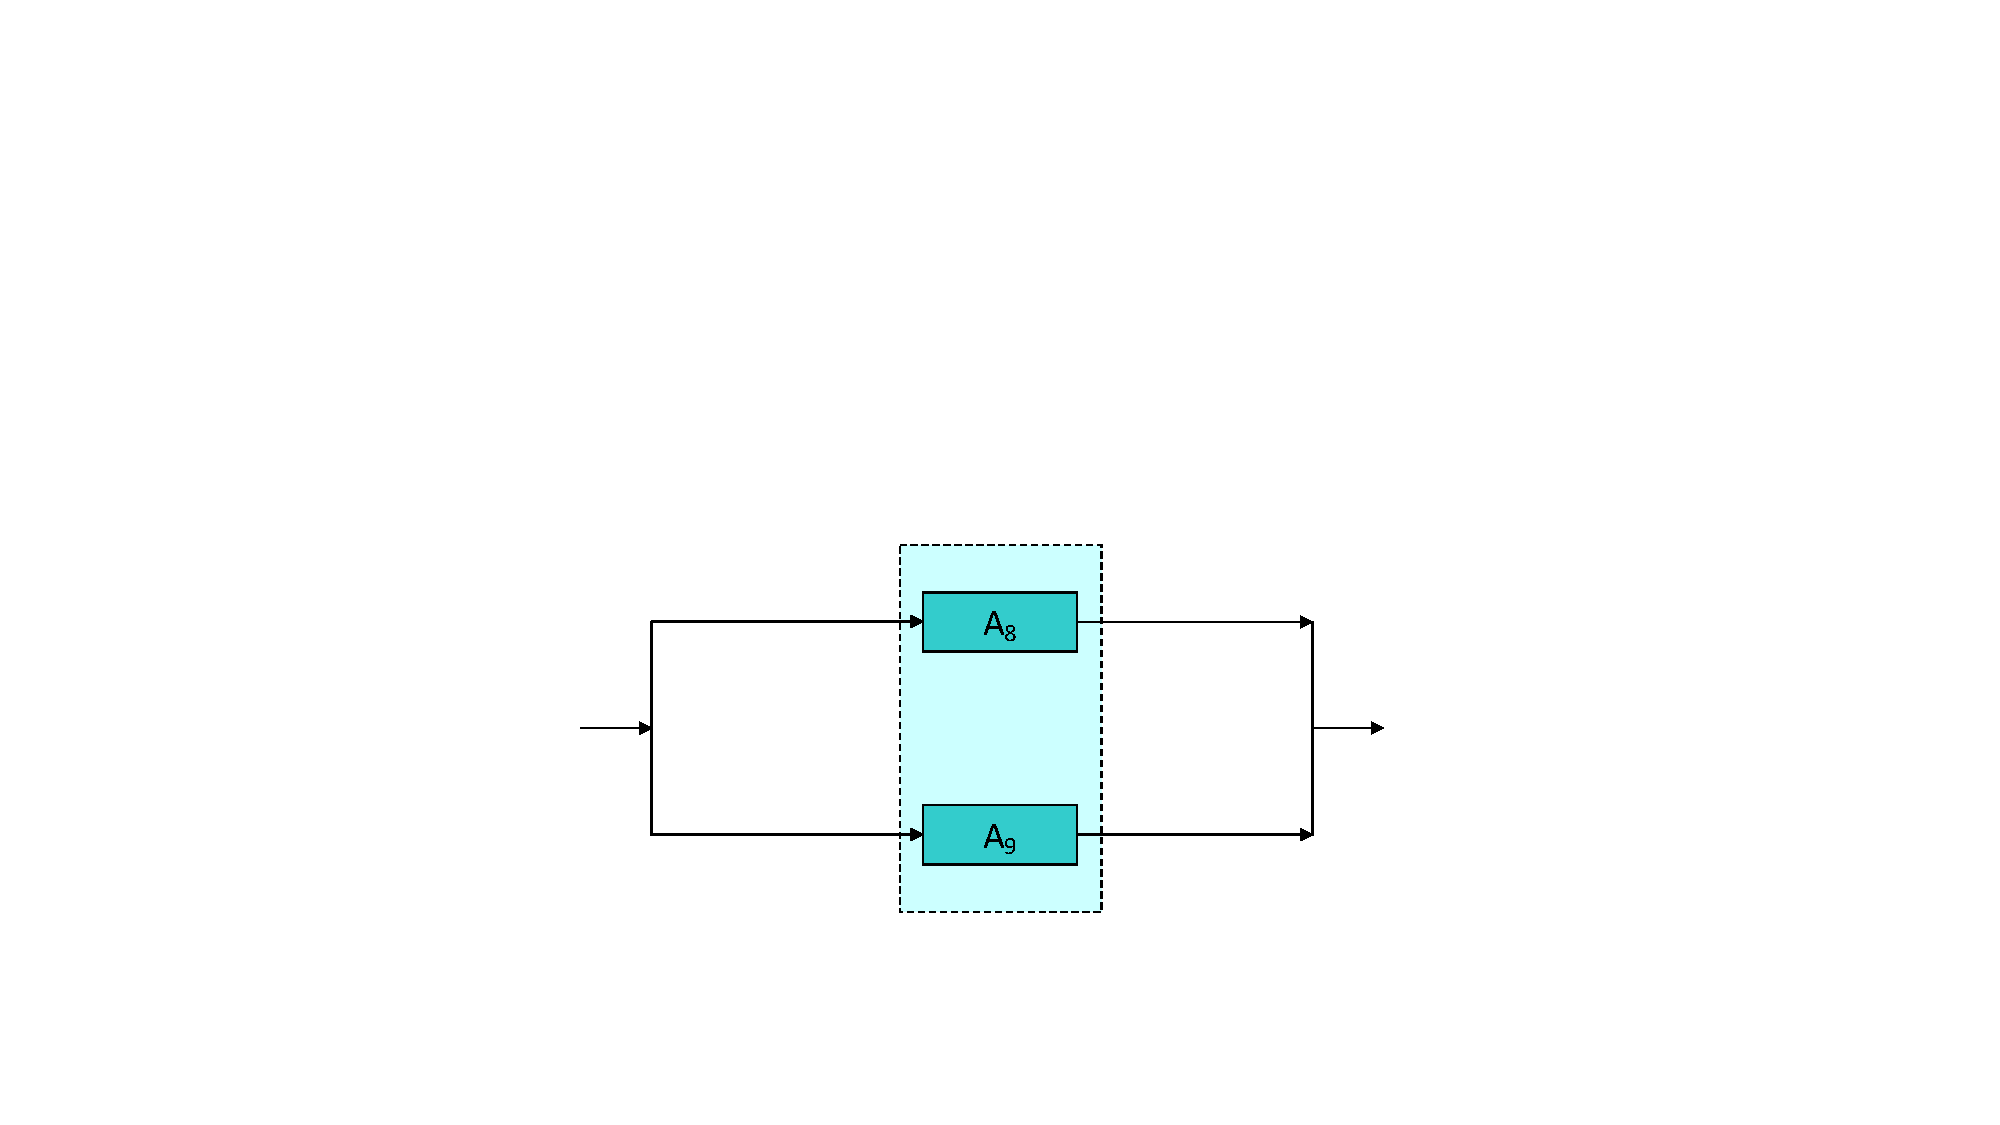
\includegraphics[width=.8\textwidth]{img/availability-in-parallel-4.pdf}
        \end{center}
    \end{itemize}
\end{examplebox}

\newpage

\begin{flushleft}
    \textcolor{Red2}{\faIcon{bookmark} \textbf{Tactics for Availability}}
\end{flushleft}
As we explained in the past pages, Availability is crucial, but it's also fundamental to use intelligent \textbf{tactics to improve the quality of the attributes}.

\begin{definitionbox}
    The \definition{Tactic}s are design decisions that influence the control of one or more quality attributes.
\end{definitionbox}

\noindent
Some well-known tactics are:
\begin{itemize}
    \item \textbf{Replication}
    \item \textbf{Forward error recovery}
    \item \textbf{Circuit breaker}
\end{itemize}

\begin{flushleft}\label{Replication approaches}
    \textcolor{Red2}{\faIcon{book} \textbf{Replication approaches}}
\end{flushleft}
The \definition{Replication} is very simple to manage in the case of stateless components. The approaches are different:
\begin{enumerate}
    \item \definition{Hot spare}: One component leads, and another is always ready to take over.
    
    In the following example, \texttt{C1} leads, \texttt{C2} is always ready to take over.
    \begin{figure}[!htp]
        \centering
        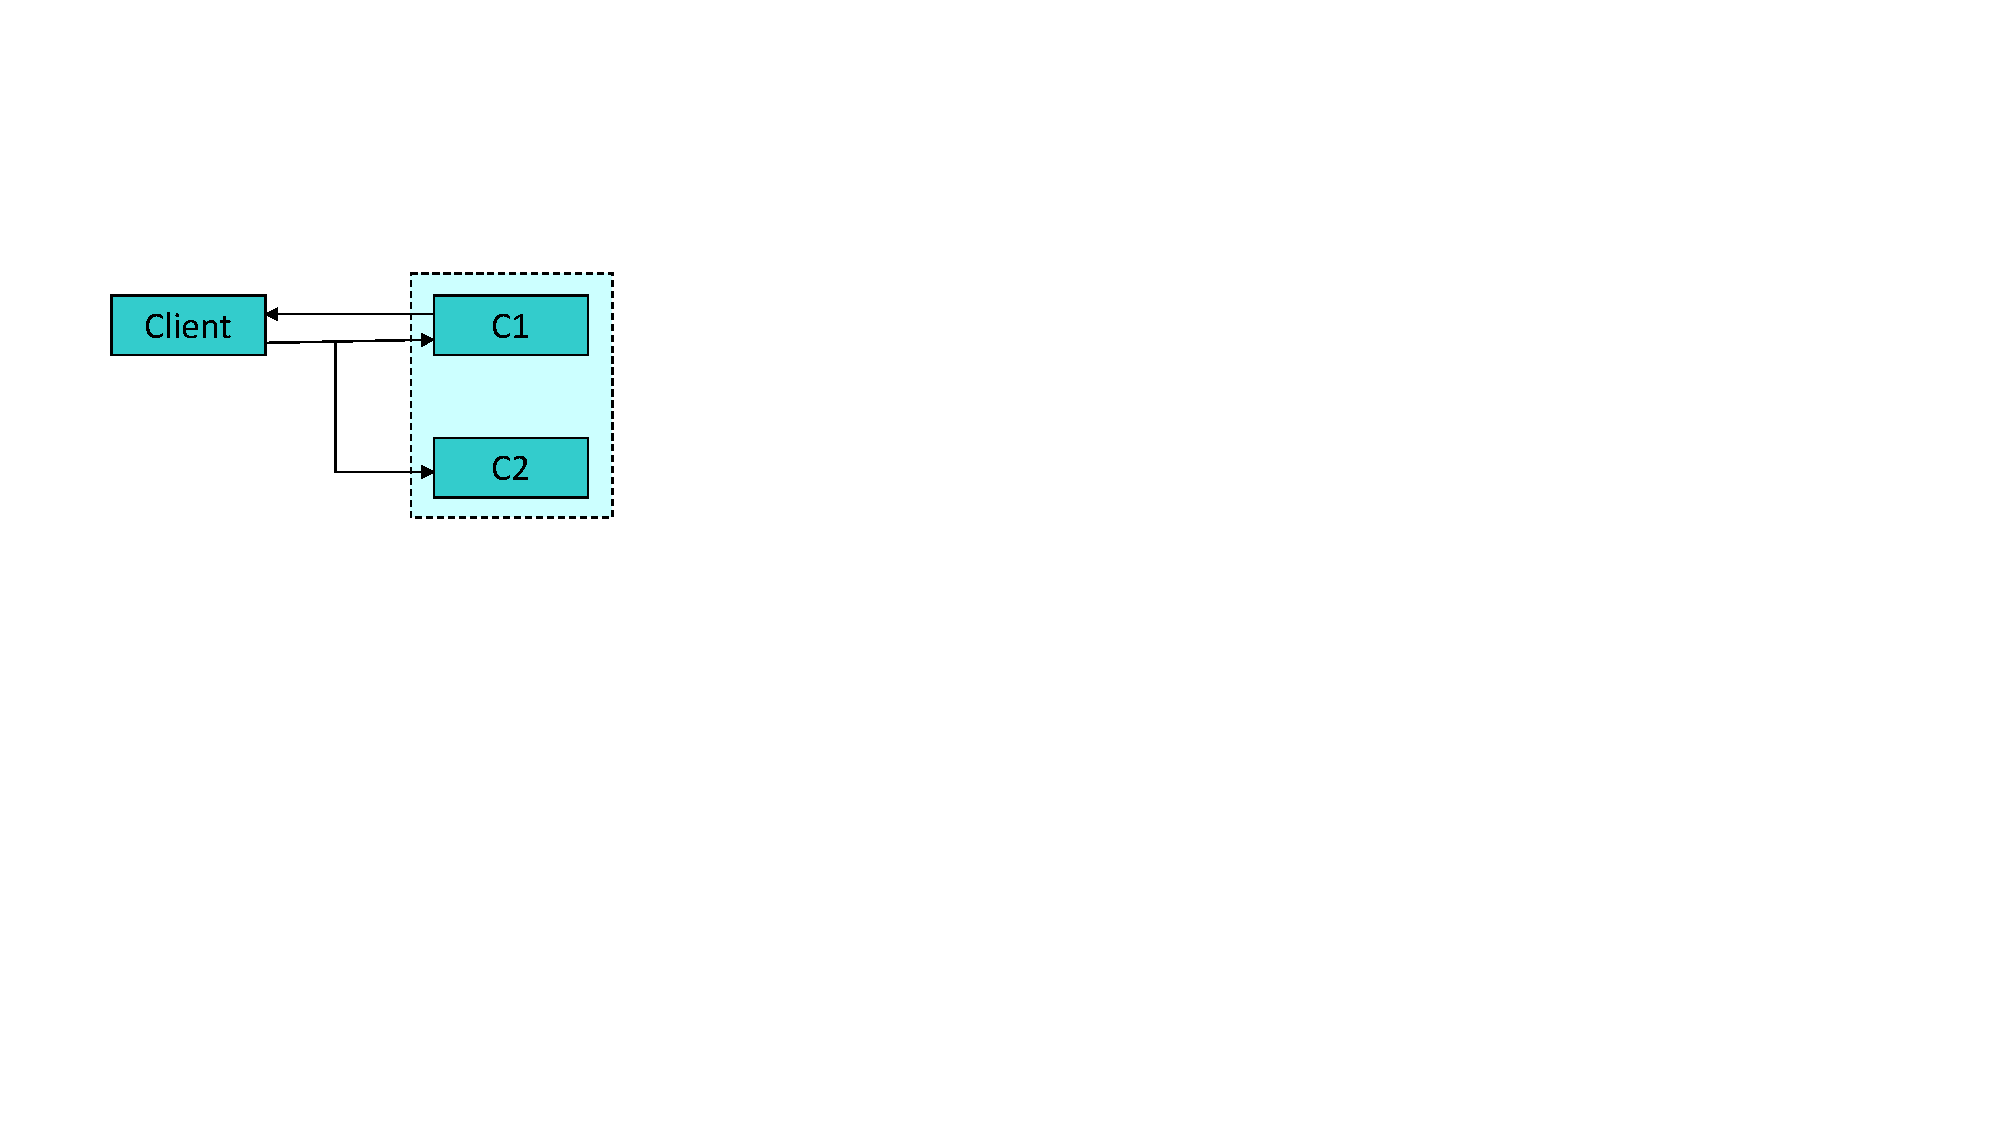
\includegraphics[width=.5\textwidth]{img/replication-1.pdf}
    \end{figure}


    \item \definition{Warm spare}: One component leads and periodically updates another component. If the primary component fails, the second component takes time to update itself fully.
    
    In the following example, \texttt{C1} leads and periodically updates \texttt{C2}. If \texttt{C1} fails, some time might be needed to fully update \texttt{C2}.
    \begin{figure}[!htp]
        \centering
        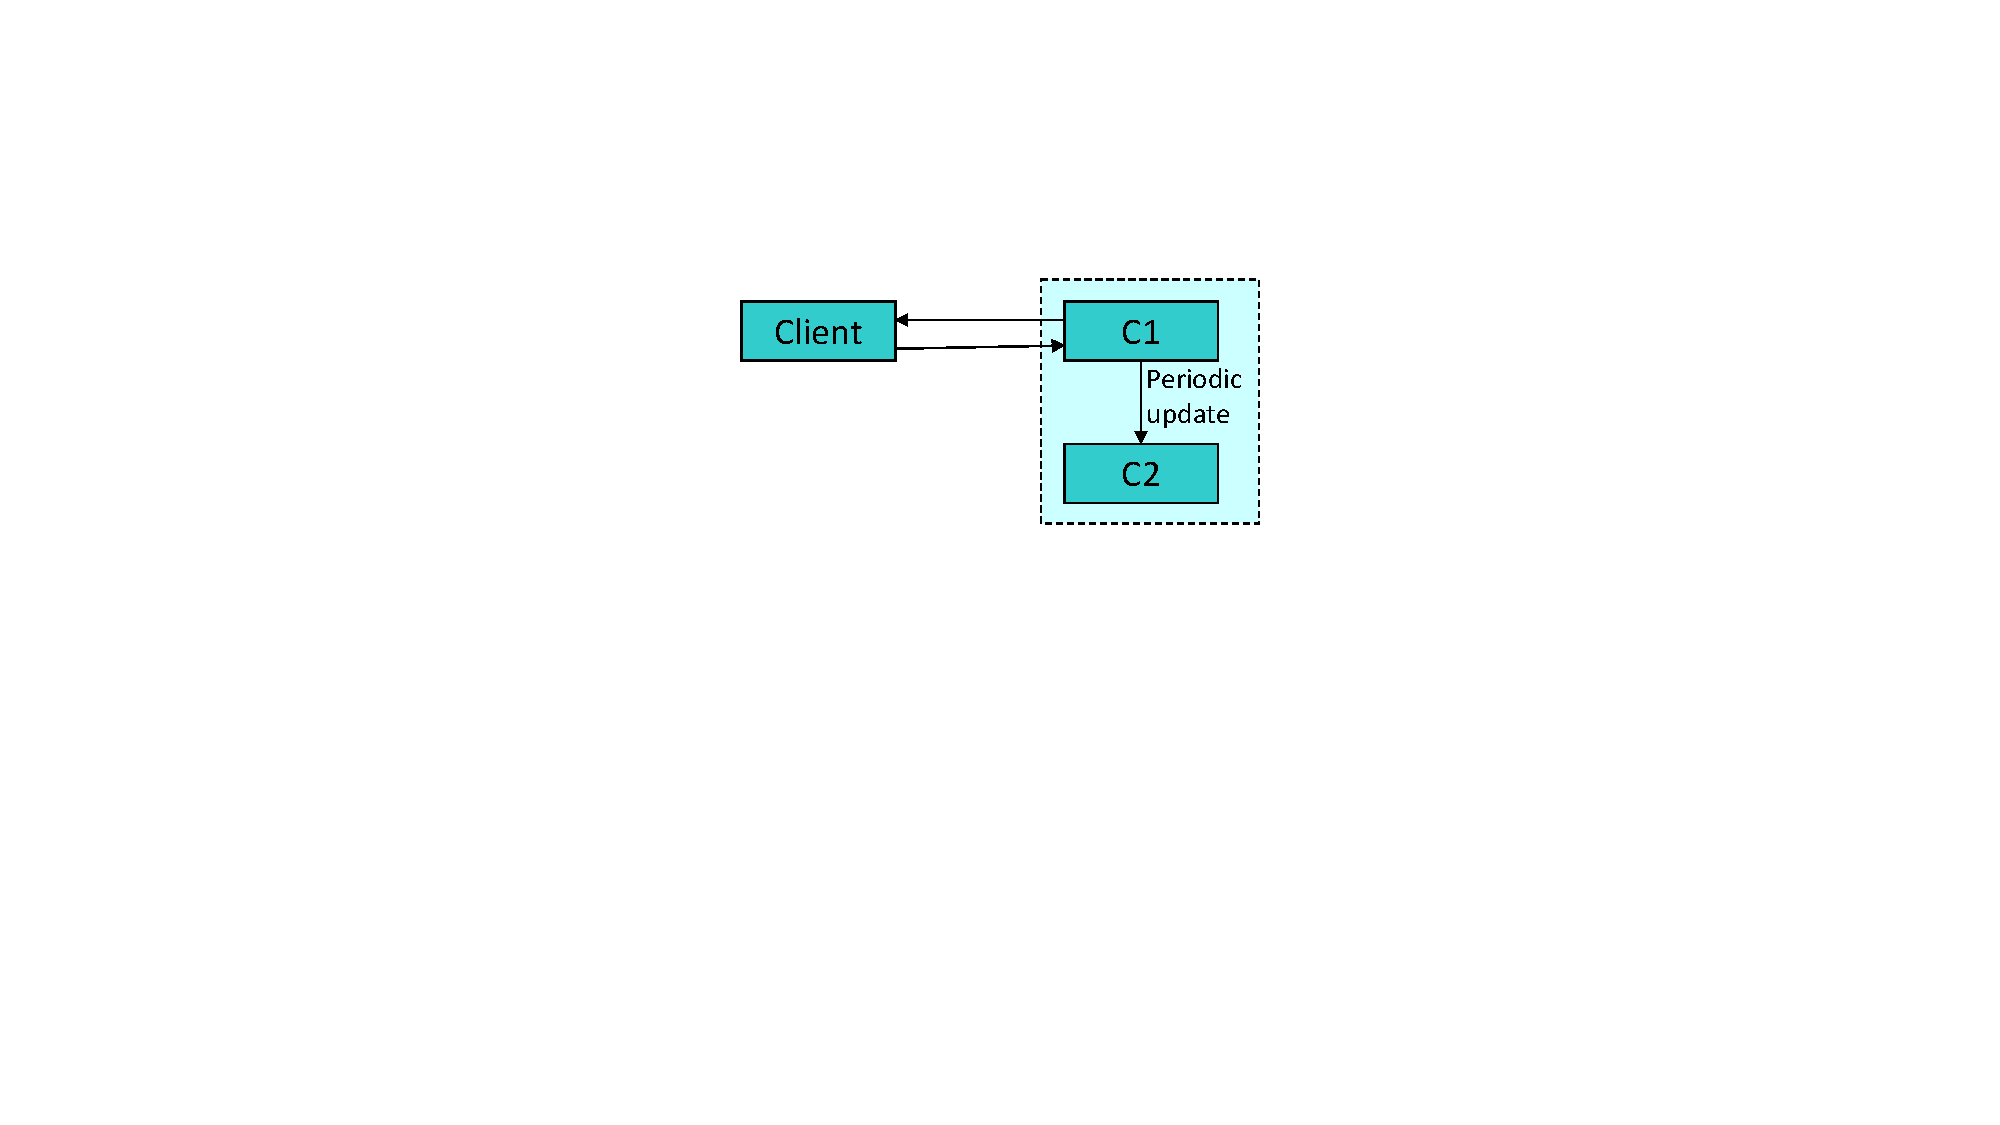
\includegraphics[width=.5\textwidth]{img/replication-2.pdf}
    \end{figure}

    \newpage

    \item \definition{Cold spare}: A second component is dormant, started, and updated only if required.

    In the following example, \texttt{C2} is dormant, started, and updated only if required.
    \begin{figure}[!htp]
        \centering
        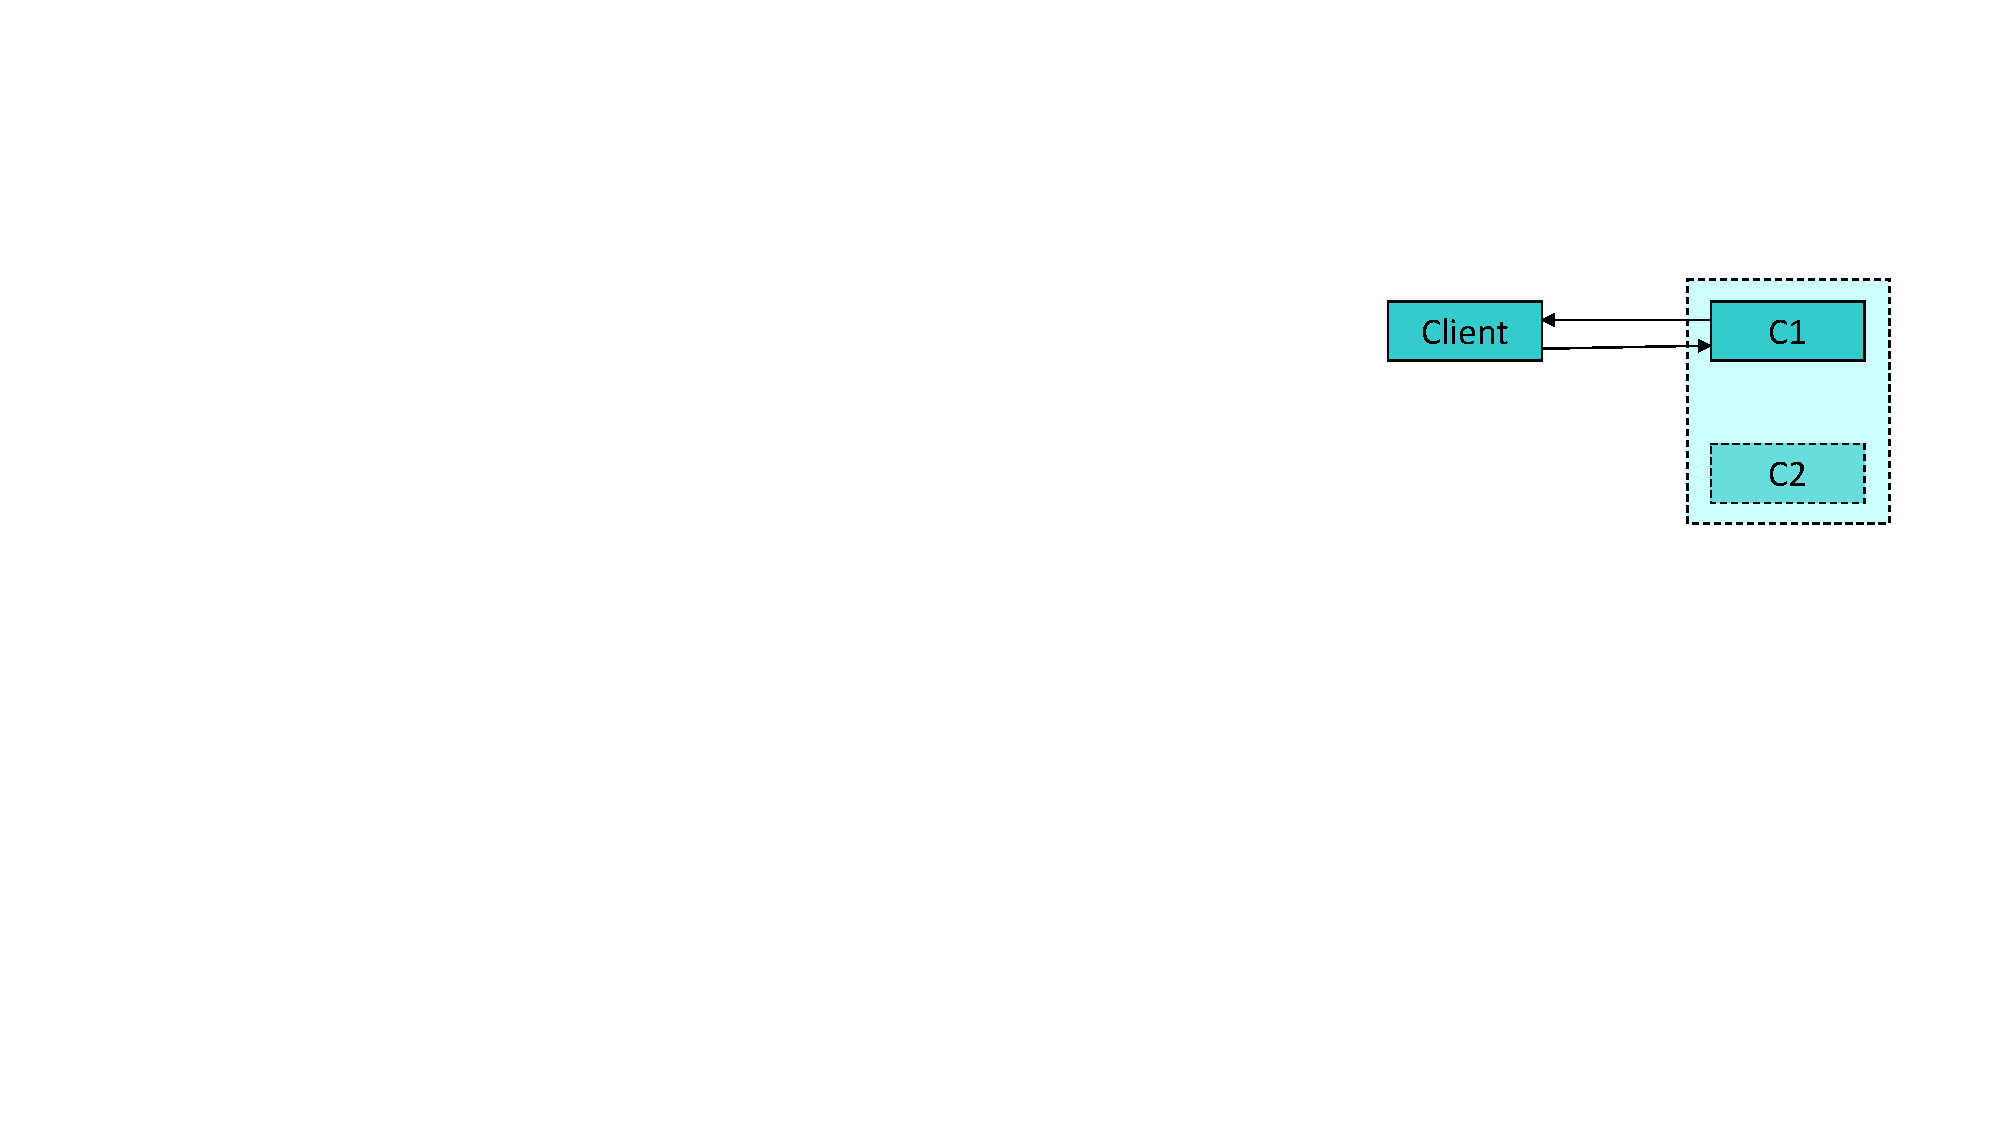
\includegraphics[width=.5\textwidth]{img/replication-3.pdf}
    \end{figure}


    \item \definition{Triple modular redundancy}: Three components are always active, and the result is the one produced by the majority. \textbf{This is good when reliability is also important}.
    
    In the following example, \texttt{C1}, \texttt{C2}, and \texttt{C3} are all active. The result is the one produced by the majority.
    \begin{figure}[!htp]
        \centering
        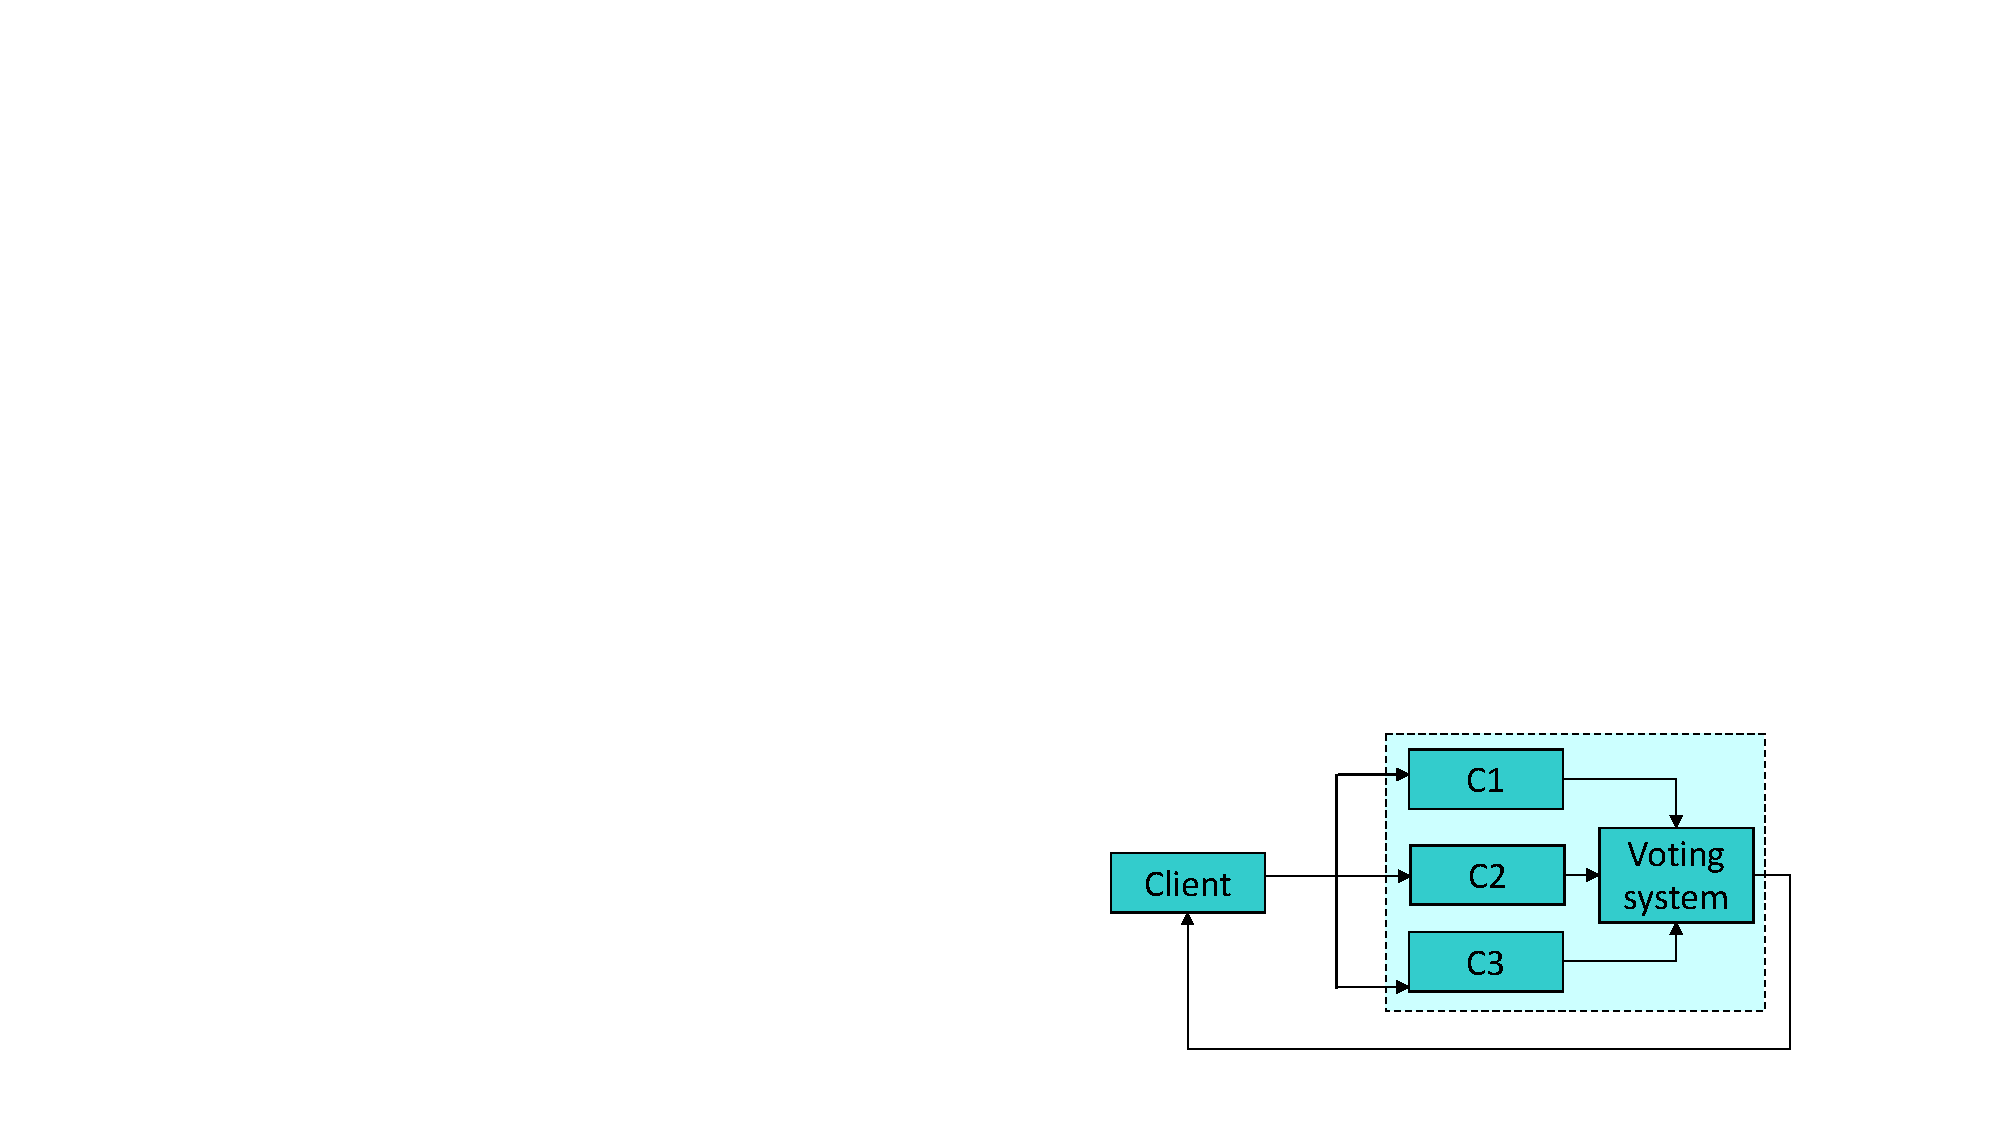
\includegraphics[width=.5\textwidth]{img/replication-4.pdf}
    \end{figure}
\end{enumerate}

\begin{flushleft}
    \textcolor{Red2}{\faIcon{book} \textbf{Forward error recovery}}
\end{flushleft}
\definition{Forward Error Recovery} is a tactic in which a recovery mechanism moves the failed component to a degraded state. In a degraded state, a component continues to be available even if it is not fully functional. Here is an example:

\begin{figure}[!htp]
    \centering
    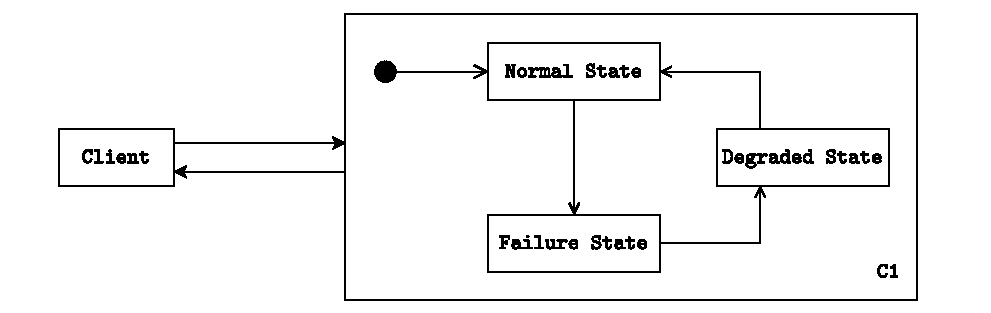
\includegraphics[width=\textwidth]{img/forward-error-recovery-1.pdf}
\end{figure}

\newpage

\begin{flushleft}
    \textcolor{Red2}{\faIcon{book} \textbf{Circuit breaker}}
\end{flushleft}
The \definition{Circuit Breaker (CB)} tactic is a client-side resiliency pattern. The CB acts as a proxy for a remote component:
\begin{enumerate}
    \item A component is called;
    \item The CB monitors the call.
\end{enumerate}
But note that there should be possible failures:
\begin{itemize}
    \item CB receives an error;
    \item The call takes \dquotes{too long} (CB kills the call).
\end{itemize}
If there are too many failures, the circuit breaker inhibits future calls by moving to the open state.

\begin{figure}[!htp]
    \centering
    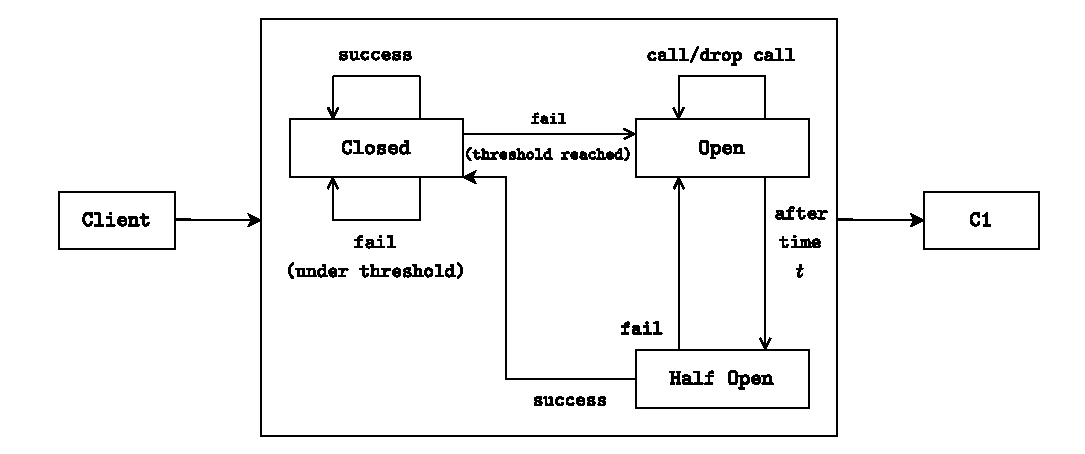
\includegraphics[width=\textwidth]{img/circuit-breaker-1.pdf}
\end{figure}
    \subsection{Analysis: Symbolic Execution}

As we have discussed in the previous subsection, there are two types of approaches when we speak about verification:
\begin{itemize}
    \item \definition{Static Analysis}. It analyzes the source code, and each analyzer targets a fixed set of hard-coded (pre-defined, not custom) properties. It is entirely automatic, and the output reports two types of results: safe (no issues) and unsafe (potential problems). Also, the \textbf{analysis is made on generic (or symbolic) inputs}.
    
    The properties that we have mentioned are safety properties, such as:
    \begin{itemize}
        \item No \emph{overflow} for integer variables
        \item No \emph{type errors}
        \item No \emph{null-pointer} dereferencing
        \item No \emph{out-of-bound} array accesses
        \item No \emph{race conditions}
        \item No \emph{useless assignments}
        \item No \emph{usage of undefined variables}
        \item No \emph{execution of specific paths}
    \end{itemize}
    
    \item Testing (dynamic analysis) is made at runtime and is related to the software's behavior during execution. The analysis is also made on specific inputs.
\end{itemize}
Using the static analysis, we can use the symbolic execution.

\begin{definitionbox}
    \definition{Symbolic Execution} (also symbolic evaluation) \textbf{analyses a program to determine what inputs cause each part of a program to execute}.
\end{definitionbox}

\noindent
The \textbf{symbolic execution} analyzes actual source code and \textbf{reachability} and \textbf{path feasibility} properties. It is automatic and may fail to explore all possible paths. Sometimes, it is used to support testing.

The checked properties by the static analysis can be of different types:
\begin{itemize}
    \item \definition{Reachability}. Does some program execution reach location $L$ (generic line of code) in S (source code)? With the reachability property, the symbolic execution tries:
    \begin{itemize}
        \item To \textbf{verify} that $L$ \textbf{cannot be reached};
        \item Or \textbf{spots the condition under which} $L$ \textbf{can be reached}.
    \end{itemize}
    For example, in the following code:
    \begin{lstlisting}
...
k:      try {
k+1:        ...
L-1:    } catch (e) {
L:          /* error */
...     }\end{lstlisting}
    Static analysis checks the reachability properties and verifies that $L$ cannot be reached, or discovers the condition under which $L$ can be reached.
    
    \item \definition{Path Feasibility}. Is the given path $p$ feasible? With the path feasibility property, the symbolic execution tries:
    \begin{itemize}
        \item To \textbf{verify} that $p$ \textbf{cannot be executed};
        \item Or \textbf{spots the condition under which} $p$ \textbf{can be executed}.
    \end{itemize}
    Then $p$ will be:
    \begin{equation*}
        p = < 0, 1, \dots, k, \dots, n >
    \end{equation*}
\end{itemize}
Symbolic execution \textbf{executes programs on symbolic values}. Each symbolic value has its \textbf{symbolic states}, which keep track of the variables' (symbolic) values. The inputs are initialized with symbolic (generic) values.

\highspace
In the following example we can see a complete example of symbolic execution. But before we do, let us introduce some \underline{\textbf{limitations}} of this methodology.
\begin{itemize}
    \item The \textbf{path conditions may be too complex for constraint solvers}. Because solvers are very good at checking linear constraints, but it is harder for them to reason about non-linear arithmetic, bit-wise operations, string manipulation, etc.
    
    \item It is \textbf{impossible} or \textbf{difficult to use when the number of paths to be explored is infinite} or \textbf{huge}. For example, unbounded loops give rise to infinite sets of paths. Although the set of paths is finite, checking all loops is expensive and impractical.
    
    \item Finally, there may be \textbf{external code}. Then the sources are not available, such as a precompiled library, or the behavior is unknown to the solver.
\end{itemize}
\begin{examplebox}
    \begin{enumerate}
        \item First we introduce the annotation:
        \begin{lstlisting}
void foo(int x, int y) {
    ...\end{lstlisting}
        \begin{center}
            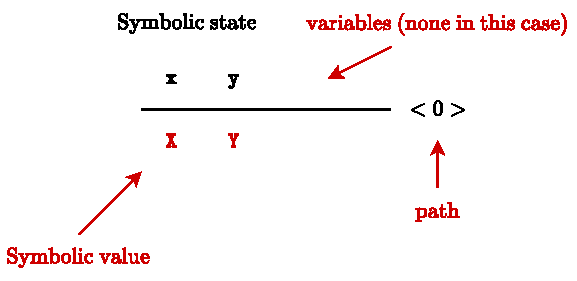
\includegraphics[width=.7\textwidth]{img/symbolic-state-1.pdf}
        \end{center}


        \item We introduce a local variable:
        \begin{lstlisting}
void foo(int x, int y) {
    int z := x\end{lstlisting}
        \begin{center}
            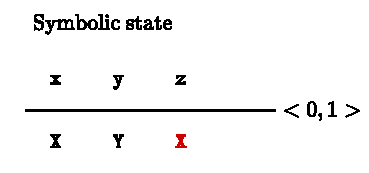
\includegraphics[width=.5\textwidth]{img/symbolic-state-2.pdf}
        \end{center}


        \item We introduce a condition. A \textbf{path condition} $\pi$ represents a constraint on a path:
        \begin{lstlisting}
void foo(int x, int y) {
    int z := x
    if (z < y)\end{lstlisting}
        \begin{itemize}
            \item if condition true
            \begin{center}
                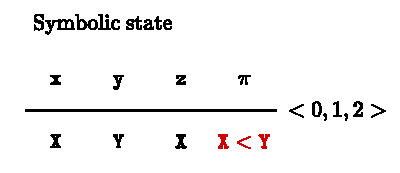
\includegraphics[width=.5\textwidth]{img/symbolic-state-3.pdf}
            \end{center}

            \item if condition false
            \begin{center}
                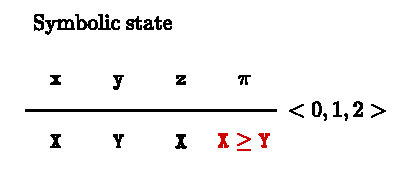
\includegraphics[width=.5\textwidth]{img/symbolic-state-4.pdf}
            \end{center}
        \end{itemize}


        \item \textbf{Execution continues along feasible paths}. In this case, the path condition $\pi$ is satisfiable:
        \begin{lstlisting}
void foo(int x, int y) {
    int z := x
    if (z < y)
        z := z*2\end{lstlisting}
        \begin{center}
            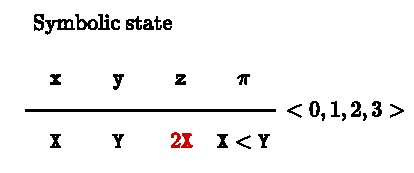
\includegraphics[width=.5\textwidth]{img/symbolic-state-5.pdf}
        \end{center}


        \item Another if condition:
        \begin{lstlisting}
void foo(int x, int y) {
    int z := x
    if (z < y)
        z := z*2
    if (x < y && z >= y)\end{lstlisting}
        \begin{itemize}
            \item if condition true
            \begin{center}
                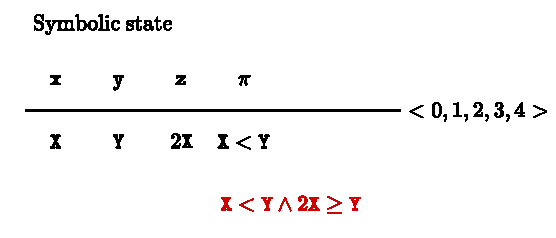
\includegraphics[width=.6\textwidth]{img/symbolic-state-6.pdf}
            \end{center}

            \item if condition false
            \begin{center}
                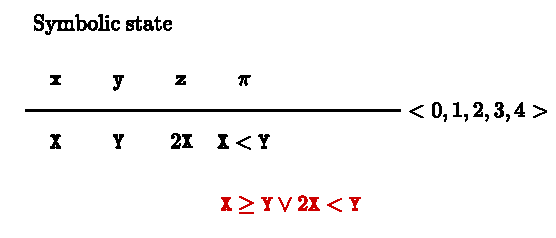
\includegraphics[width=.6\textwidth]{img/symbolic-state-7.pdf}
            \end{center}
        \end{itemize}


        \item Possible outcomes of symbolic execution:
        \begin{lstlisting}
void foo(int x, int y) {
    int z := x
    if (z < y)
        z := z*2
    if (x < y && z >= y)
        print(z)
}\end{lstlisting}
        \begin{enumerate}
            \item \textcolor{Green3}{\textbf{Satisfiable}} exit ($\pi$ is satisfiable): every satisfying assignment to variables in $\pi$ is an \textbf{input that satisfies the given property in a concrete execution}.
            \begin{center}
                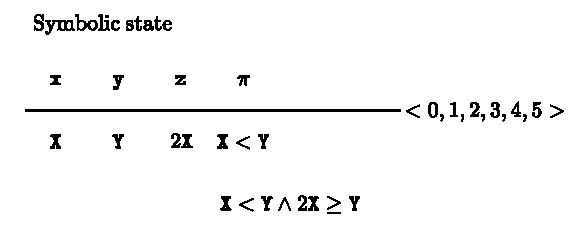
\includegraphics[width=.6\textwidth]{img/symbolic-state-8.pdf}
            \end{center}


            \item \textcolor{Red2}{\textbf{Unsatisfiable}} exit ($\pi$ is not satisfiable): the given \textbf{property cannot be satisfied by any concrete execution}.
            \begin{center}
                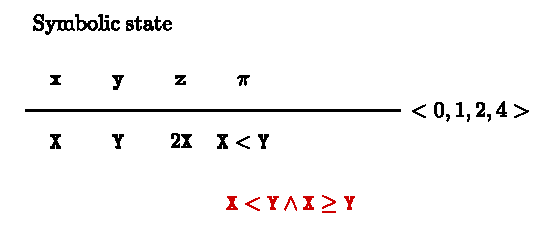
\includegraphics[width=.6\textwidth]{img/symbolic-state-9.pdf}
            \end{center}
        \end{enumerate}
    \end{enumerate}
    Finally, we can draw the \definition{Execution Tree}. The execution paths can be collected in an execution tree, where end states are marked as \texttt{SAT} or \texttt{UNSAT}.
    \begin{center}
        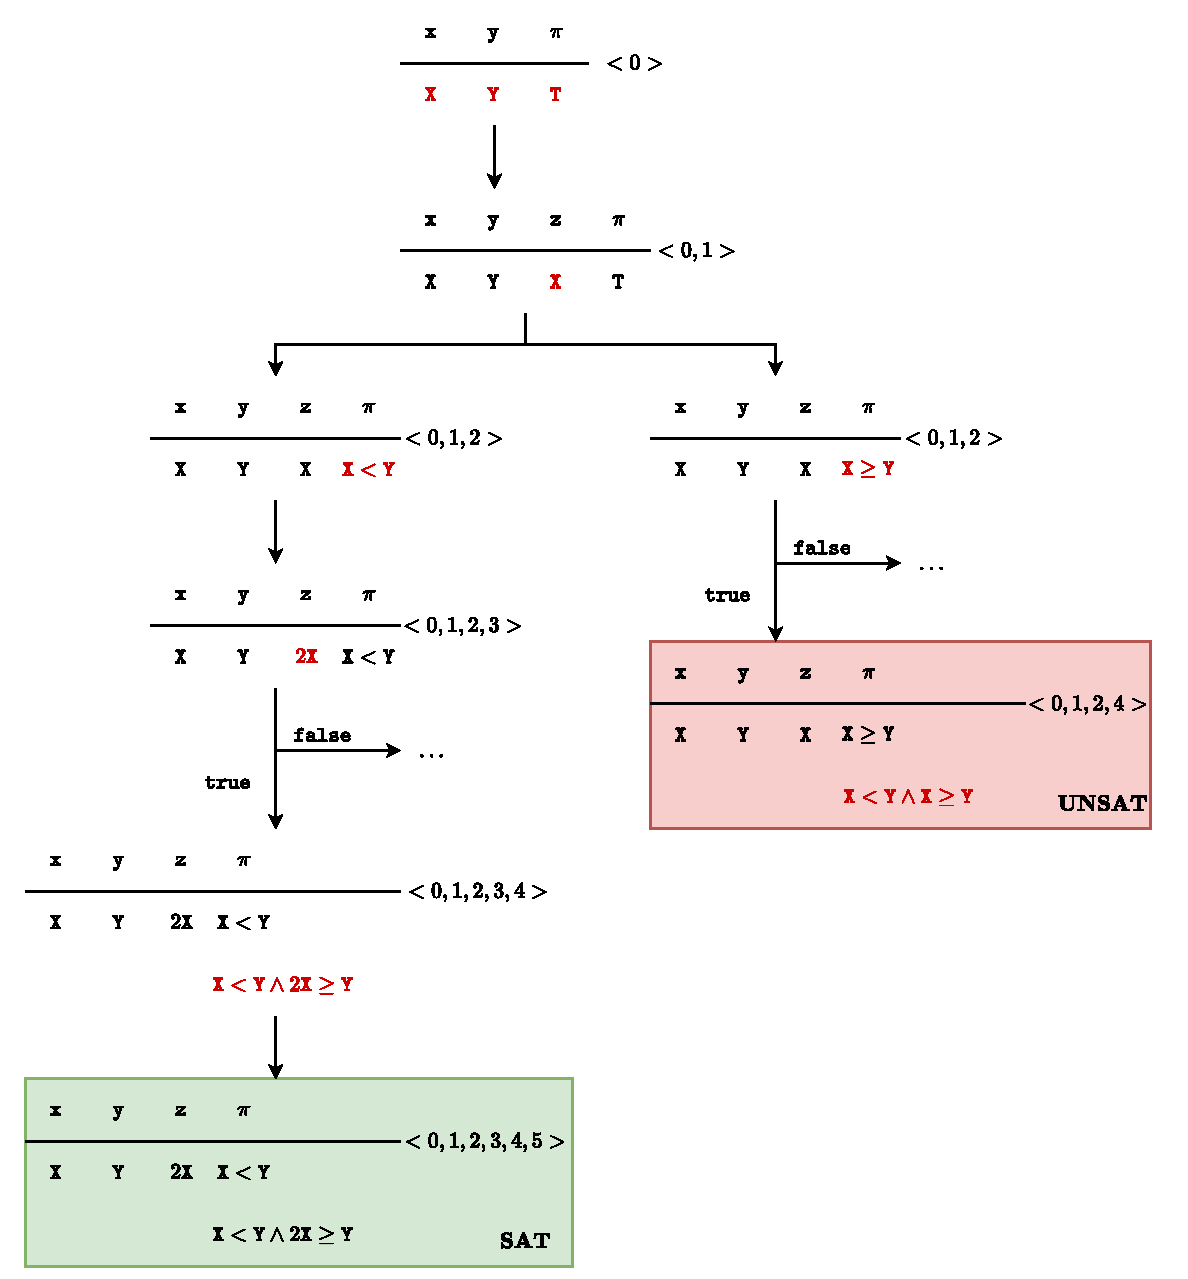
\includegraphics[width=\textwidth]{img/symbolic-state-10.pdf}
    \end{center}
    To view the tree in high resolution, scan (or click) the QR code below.
    \begin{center}
        \qrcode{https://github.com/PoliMI-HPC-E-notes-projects-AndreVale69/HPC-E-PoliMI-university-notes/tree/main/software-engineering-for-hpc/notes/img/symbolic-state-10.pdf}
    \end{center}
\end{examplebox}

\newpage

\subsection{Testing: terminology, types of testing activities}

\definition{Testing} (dynamic analysis) is an approach to verification. The \textbf{main goal of testing is to make programs fail}.

Other \emph{common goals} are:
\begin{itemize}
    \item Exercise different parts of a program to \textbf{increase coverage};
    
    \item Make sure the \textbf{interaction between components works} (\emph{integration testing});
    
    \item Support \textbf{fault localization} and \textbf{error removal} (\emph{debugging});
    
    \item Ensure that \textbf{bugs introduced in the past do not happen again} (\emph{regression testing}).
\end{itemize}
The dynamic analysis \textbf{analyzes program behavior}. The \textbf{properties} are \textbf{encoded as executable oracles representing expected outputs} and \textbf{desired conditions} (assertions).

It can \textbf{run only finite test cases}, so it's not exhaustive verification. The \textbf{failures have concrete inputs that trigger them}, and the \textbf{execution is automatic}.

\begin{flushleft}
    \textcolor{Green3}{\faIcon{question-circle} \textbf{We have often heard about \emph{debugging}, but what is it?}}
\end{flushleft}
\definition{Debugging} is a systematic approach to \textbf{fault localization and error removal}. The output is often used to support debugging.

\begin{figure}[!htp]
    \centering
    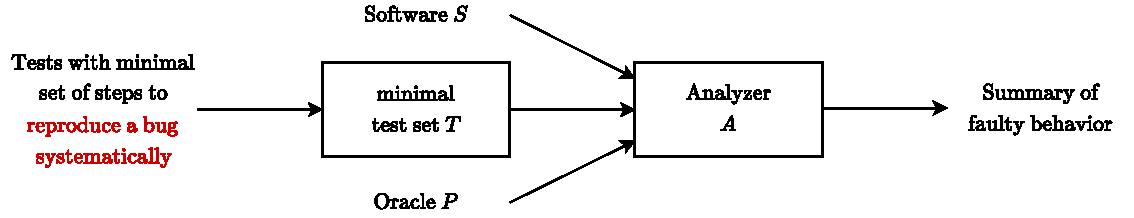
\includegraphics[width=\textwidth]{img/testing-1.pdf}
\end{figure}

\begin{flushleft}
    \textcolor{Green3}{\faIcon{question-circle} \textbf{... and \emph{test case}?}}
\end{flushleft}
\begin{definitionbox}
    A \definition{Test Case} is a set of \textbf{inputs}, \textbf{execution conditions}, and a \textbf{pass/fail criterion}.
\end{definitionbox}

\noindent
Running a test case typically involves setup, execution and teardown.
\begin{itemize}
    \item \textbf{Setup}. Bring the program to an \textbf{initial state} that fulfils the execution conditions.
    
    \item \textbf{Execution}. \textbf{Run} the program on the actual inputs.
    
    \item \textbf{Teardown}. \textbf{Record} the output, the final state, and any \textbf{failure} determined based on the pass/fail criterion.
\end{itemize}
A \textbf{test set}, or \textbf{test suite}, can include \textbf{multiple test cases}. Finally, a \definition{Test Case Specification} is a \textbf{requirement to be satisfied by one or more test cases}. An example of test case specification can be \emph{the input must be a sentence composed of at least two words}, and an example of test case input is \emph{this is a good test case input}.

\highspace
When discussing test cases, it's necessary to introduce \definition{Unit Testing}. This is \textbf{conducted by developers} and \textbf{aims to test small pieces} (units) \textbf{of code in isolation}. 

However, when we test in isolation, there should be a \textbf{problem}: the \textbf{units may depend on other units}. Then, we need to simulate missing units.

\highspace
The \definition{Integration Testing} (integration of the unit tests) \textbf{aims to exercise the interaction between interfaces and components}. The \textbf{faults} discovered by integration testing are multiple; some examples:
\begin{itemize}
    \item \textbf{Inconsistent interpretation of parameters} (e.g. mixed units meters or yards)

    \item \textbf{Violations of assumptions about domains} (e.g. buffer overflow)

    \item \textbf{Side effects on parameters or resources} (e.g. conflict on temporary file)

    \item \textbf{Nonfunctional properties} (e.g. unanticipated performance issues)

    \item \textbf{Concurrency-specific problems}
\end{itemize}
Typically, the integration test is defined by the Design Document. In the Design Document, we can find two types of plans:
\begin{itemize}
    \item \definition{Build Plan} that establishes the \textbf{order of the implementation};
    \item A \definition{Test Plan} that defines how to carry out integration testing is needed.
\end{itemize}
The strategies for the integration test are many:
\begin{itemize}
    \item \definition{Big Bang}: \textbf{test only after integrating all modules} (not even a real strategy). 
    
    \begin{flushleft}
        \textcolor{Green3}{\faIcon{check} \textbf{Pros}}
    \end{flushleft}
    It doesn't require stubs; it only \textbf{requires fewer drivers}/\textbf{oracles}.
    
    \begin{flushleft}
        \textcolor{Red2}{\faIcon{exclamation-triangle} \textbf{Cons}}
    \end{flushleft}
    \begin{enumerate}
        \item Minimum: observability, fault localization/diagnosability, efficacy, feedback;
        \item \textbf{High cost of repair} (cost of repairing a fault increases as a function of time between the introduction of an error in the code and repair).
    \end{enumerate}

    \newpage


    \item \definition{Iterative and incremental strategies}. The main action is \textbf{run after components are released (not just at the end)}. The strategy can be done in three different ways:
    \begin{itemize}
        \item \textbf{Hierarchical}. Based on the hierarchical structure of the system. It can be done top-down or bottom-up.
        \begin{itemize}
            \item \textbf{\emph{Top-down} strategy}. Work \textbf{from the top level} (in terms of \dquotes{use} or \dquotes{include} relationship) \textbf{down to the bottom level}. As modules are completed (according to the building plan), more functionality is testable. We also need to replace some stubs, and we need other stubs for lower levels. \textbf{When all modules are incorporated, the whole functionality can be tested}.
            
            \highspace
            \begin{flushleft}
                \textcolor{Green3}{\faIcon{check} \textbf{Pros}}
            \end{flushleft}
            The drivers use the top level interfaces (e.g. REST APIs).
            
            \highspace
            \begin{flushleft}
                \textcolor{Red2}{\faIcon{exclamation-triangle} \textbf{Cons}}
            \end{flushleft}
            This strategy requires stubs of used modules at each step of the process.

            \begin{figure}[!htp]
                \centering
                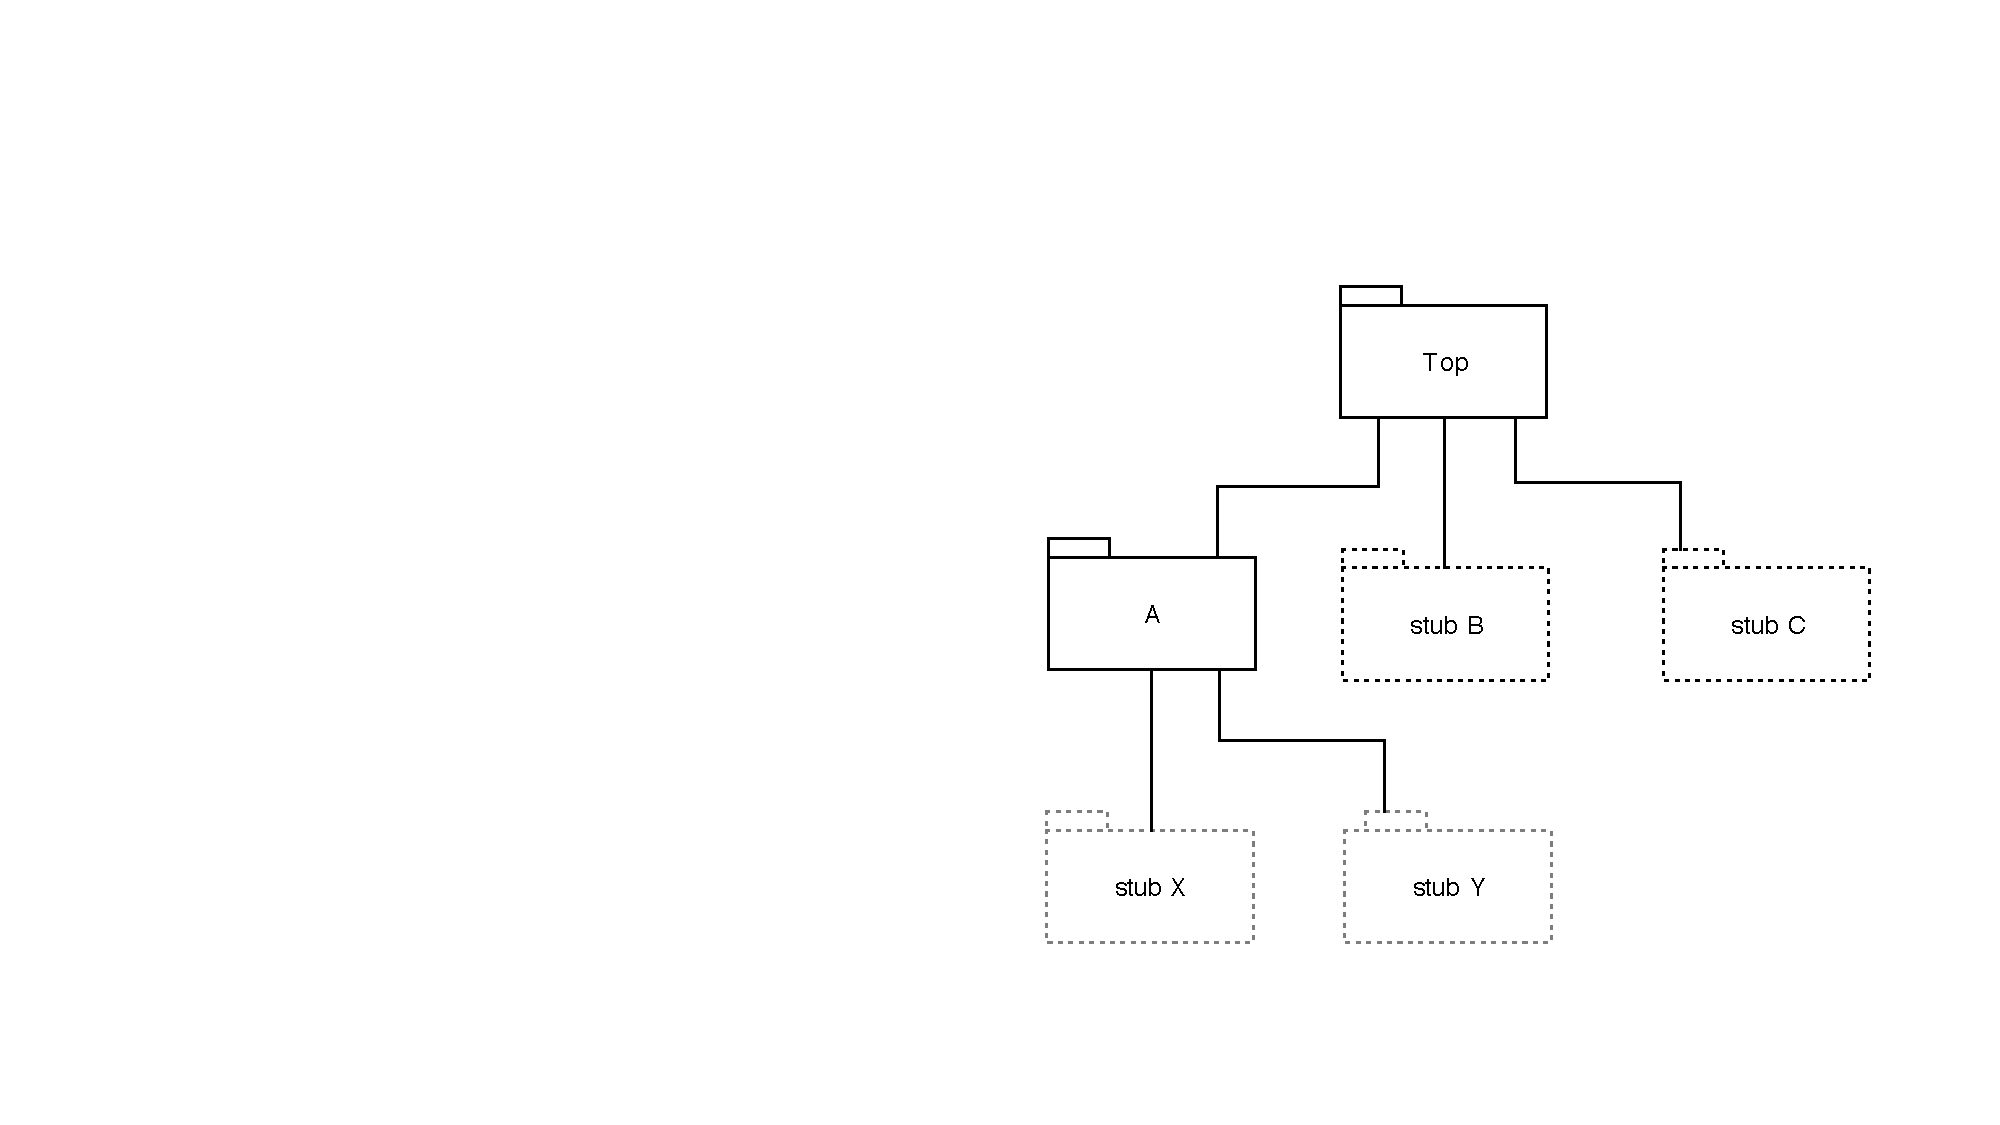
\includegraphics[width=.6\textwidth]{img/top-down-1.pdf}
                \caption{\example{Example} of top-down strategy.}
            \end{figure}
            
            \newpage

            \item \textbf{\emph{Bottom-up} strategy}. Starting from the leaves of the \dquotes{uses} hierarchy. 
            
            \highspace
            \begin{flushleft}
                \textcolor{Green3}{\faIcon{check} \textbf{Pros}}
            \end{flushleft}
            An advantage is that it \textbf{doesn't require stubs}.
            
            \highspace
            \begin{flushleft}
                \textcolor{Red2}{\faIcon{exclamation-triangle} \textbf{Cons}}
            \end{flushleft}
            \textbf{Typically requires more drivers} (one for each module, as in unit testing). Can this be a disadvantage? Maybe, because the newly developed module may replace an existing driver, and new modules require new drivers.

            Another thing to consider is that \textbf{it may create several working subsystems}, and each working subsystem will eventually be integrated into the final one.

            \begin{figure}[!htp]
                \centering
                \includegraphics[width=.6\textwidth]{img/bottom-up-1.pdf}
                \caption{\example{Example} of bottom-up strategy.}
            \end{figure}
        \end{itemize}

        \newpage

        \item \textbf{Threads}. A \textbf{thread is a part of several modules that together provide a user-visible programme function}. By using the thread strategy we can have some \textbf{advantages}.
        \begin{flushleft}
            \textcolor{Green3}{\faIcon{check} \textbf{Pros}}
        \end{flushleft}
        \begin{itemize}
            \item We can \textbf{maximize the progress visible to the user} (or other stakeholders);
            \item \textbf{Reduce drivers and stubs};
            \item An integration plan is usually more complex.
        \end{itemize}
        \begin{figure}[!htp]
            \centering
            \includegraphics[width=.6\textwidth]{img/threads-1.pdf}
            \caption{\example{Example} of threads strategy.}
        \end{figure}
        
        \item \textbf{Critical}. The critical modules strategy \textbf{starts with the highest risk modules}. Risk assessment is a necessary first step. It can include technical risks (e.g. is X feasible?) and process risks (e.g. is the schedule for X realistic?). It may also be similar to a priority process.

        The \textbf{key point of this strategy is the risk-oriented process}. Integration and testing as a risk mitigation activity, designed to \emph{deliver any bad news as early as possible}.
    \end{itemize}
\end{itemize}

\begin{flushleft}
    \textcolor{Green3}{\faIcon{question-circle} \textbf{Which one should we choose?}}
\end{flushleft}
Given the three strategies above, \emph{which one should we choose}? Well, the structural strategies (bottom-up or top-down) are simpler, but thread and critical modules provide better external visibility of progress (especially in complex systems).

\highspace
So the \textbf{best choice} should be a \textbf{combination of different strategies}:
- Use \textbf{top-down/bottom-up} for relatively \textbf{small components} and \textbf{subsystems};
- Combinations of \textbf{thread} and \textbf{critical module integration testing} for \textbf{larger subsystems}.

\newpage

\subsubsection{E2E Testing}

\begin{definitionbox}
    \definition{End-to-end (E2E)} testing is a \textbf{software testing methodology to test a functional and data application flow consisting of several sub-systems working together from start to end}.\footnote{\href{https://microsoft.github.io/code-with-engineering-playbook/automated-testing/e2e-testing/}{Engineering Fundamentals Playbook}}
\end{definitionbox}

\noindent
At times, these systems are developed in different technologies by different teams or organizations. Finally, they come together to form a functional business application. Hence, testing a single system would not suffice. Therefore, end-to-end testing verifies the application from start to end putting all its components together.

\highspace
The following is a list of \textbf{common types of tests} that use the E2E system:
\begin{itemize}
    \item \definition{Functional Testing}
    \begin{flushleft}
        \textcolor{Red2}{\faIcon{book} \textbf{Purpose}}
    \end{flushleft}
    Check whether the \textbf{software meets the functional requirements}.

    \begin{flushleft}
        \textcolor{Green3}{\faIcon{question-circle} \textbf{How?}}
    \end{flushleft}
    Use the software as described by use cases in the RASD (pag. \pageref{RASD}), check whether requirements are fulfilled.


    \item \definition{Performance Testing}
    \begin{flushleft}
        \textcolor{Red2}{\faIcon{book} \textbf{Purpose}}
    \end{flushleft}
    \begin{enumerate}
        \item Detect \textbf{bottlenecks} affecting response time, utilization, throughput
        \item Detect \textbf{inefficient algorithms}
        \item Detect \textbf{hardware/network issues}
        \item Identify \textbf{optimization possibilities}
    \end{enumerate}

    \begin{flushleft}
        \textcolor{Green3}{\faIcon{question-circle} \textbf{How?}}
    \end{flushleft}
    Load the system with the expected workload and measure and compare acceptable performance.
    
    \newpage

    \item \definition{Load Testing}
    \begin{flushleft}
        \textcolor{Red2}{\faIcon{book} \textbf{Purpose}}
    \end{flushleft}
    \begin{enumerate}
        \item \textbf{Expose bugs} such as memory leaks, mismanagement of memory, buffer overflows
        \item Identify \textbf{upper limits of components}
        \item \textbf{Compare alternative architectural options}
    \end{enumerate}

    \begin{flushleft}
        \textcolor{Green3}{\faIcon{question-circle} \textbf{How?}}
    \end{flushleft}
    Test the system at increasing workload until it can support it, and load the system for a long period.


    \item \definition{Stress Testing}
    \begin{flushleft}
        \textcolor{Red2}{\faIcon{book} \textbf{Purpose}}
    \end{flushleft}
    Make sure that the \textbf{system recovers gracefully after failure}.

    \begin{flushleft}
        \textcolor{Green3}{\faIcon{question-circle} \textbf{How?}}
    \end{flushleft}
    Trying to break the system under the test by overwhelming its resources or by reducing resources.

    For \example{example} double the baseline number for concurrent users/HTTP connections, or randomly shut down and restart ports on the network switches/routers that connect servers.
\end{itemize}
    \subsection{Testing: terminology, types of testing activities}

\definition{Testing} (dynamic analysis) is an approach to verification. The \textbf{main goal of testing is to make programs fail}.

Other \emph{common goals} are:
\begin{itemize}
    \item Exercise different parts of a program to \textbf{increase coverage};
    
    \item Make sure the \textbf{interaction between components works} (\emph{integration testing});
    
    \item Support \textbf{fault localization} and \textbf{error removal} (\emph{debugging});
    
    \item Ensure that \textbf{bugs introduced in the past do not happen again} (\emph{regression testing}).
\end{itemize}
The dynamic analysis \textbf{analyzes program behavior}. The \textbf{properties} are \textbf{encoded as executable oracles representing expected outputs} and \textbf{desired conditions} (assertions).

It can \textbf{run only finite test cases}, so it's not exhaustive verification. The \textbf{failures have concrete inputs that trigger them}, and the \textbf{execution is automatic}.

\begin{flushleft}
    \textcolor{Green3}{\faIcon{question-circle} \textbf{We have often heard about \emph{debugging}, but what is it?}}
\end{flushleft}
\definition{Debugging} is a systematic approach to \textbf{fault localization and error removal}. The output is often used to support debugging.

\begin{figure}[!htp]
    \centering
    \includegraphics[width=\textwidth]{img/testing-1.pdf}
\end{figure}

\begin{flushleft}
    \textcolor{Green3}{\faIcon{question-circle} \textbf{... and \emph{test case}?}}
\end{flushleft}
\begin{definitionbox}
    A \definition{Test Case} is a set of \textbf{inputs}, \textbf{execution conditions}, and a \textbf{pass/fail criterion}.
\end{definitionbox}

\noindent
Running a test case typically involves setup, execution and teardown.
\begin{itemize}
    \item \textbf{Setup}. Bring the program to an \textbf{initial state} that fulfils the execution conditions.
    
    \item \textbf{Execution}. \textbf{Run} the program on the actual inputs.
    
    \item \textbf{Teardown}. \textbf{Record} the output, the final state, and any \textbf{failure} determined based on the pass/fail criterion.
\end{itemize}
A \textbf{test set}, or \textbf{test suite}, can include \textbf{multiple test cases}. Finally, a \definition{Test Case Specification} is a \textbf{requirement to be satisfied by one or more test cases}. An example of test case specification can be \emph{the input must be a sentence composed of at least two words}, and an example of test case input is \emph{this is a good test case input}.

\highspace
When discussing test cases, it's necessary to introduce \definition{Unit Testing}. This is \textbf{conducted by developers} and \textbf{aims to test small pieces} (units) \textbf{of code in isolation}. 

However, when we test in isolation, there should be a \textbf{problem}: the \textbf{units may depend on other units}. Then, we need to simulate missing units.

\highspace
The \definition{Integration Testing} (integration of the unit tests) \textbf{aims to exercise the interaction between interfaces and components}. The \textbf{faults} discovered by integration testing are multiple; some examples:
\begin{itemize}
    \item \textbf{Inconsistent interpretation of parameters} (e.g. mixed units meters or yards)

    \item \textbf{Violations of assumptions about domains} (e.g. buffer overflow)

    \item \textbf{Side effects on parameters or resources} (e.g. conflict on temporary file)

    \item \textbf{Nonfunctional properties} (e.g. unanticipated performance issues)

    \item \textbf{Concurrency-specific problems}
\end{itemize}
Typically, the integration test is defined by the Design Document. In the Design Document, we can find two types of plans:
\begin{itemize}
    \item \definition{Build Plan} that establishes the \textbf{order of the implementation};
    \item A \definition{Test Plan} that defines how to carry out integration testing is needed.
\end{itemize}
The strategies for the integration test are many:\index{Strategies for the integration test}
\begin{itemize}
    \item \definition{Big Bang}: \textbf{test only after integrating all modules} (not even a real strategy). 
    
    \begin{flushleft}
        \textcolor{Green3}{\faIcon{check} \textbf{Pros}}
    \end{flushleft}
    It doesn't require stubs; it only \textbf{requires fewer drivers}/\textbf{oracles}.
    
    \begin{flushleft}
        \textcolor{Red2}{\faIcon{exclamation-triangle} \textbf{Cons}}
    \end{flushleft}
    \begin{enumerate}
        \item Minimum: observability, fault localization/diagnosability, efficacy, feedback;
        \item \textbf{High cost of repair} (cost of repairing a fault increases as a function of time between the introduction of an error in the code and repair).
    \end{enumerate}

    \newpage


    \item \definition{Iterative and incremental strategies}. The main action is \textbf{run after components are released (not just at the end)}. The strategy can be done in three different ways:
    \begin{itemize}
        \item \textbf{Hierarchical}. Based on the hierarchical structure of the system. It can be done top-down or bottom-up.
        \begin{itemize}
            \item \textbf{\emph{Top-down} strategy}. Work \textbf{from the top level} (in terms of \dquotes{use} or \dquotes{include} relationship) \textbf{down to the bottom level}. As modules are completed (according to the building plan), more functionality is testable. We also need to replace some stubs, and we need other stubs for lower levels. \textbf{When all modules are incorporated, the whole functionality can be tested}.
            
            \highspace
            \begin{flushleft}
                \textcolor{Green3}{\faIcon{check} \textbf{Pros}}
            \end{flushleft}
            The drivers use the top level interfaces (e.g. REST APIs).
            
            \highspace
            \begin{flushleft}
                \textcolor{Red2}{\faIcon{exclamation-triangle} \textbf{Cons}}
            \end{flushleft}
            This strategy requires stubs of used modules at each step of the process.

            \begin{figure}[!htp]
                \centering
                \includegraphics[width=.6\textwidth]{img/top-down-1.pdf}
                \caption{\example{Example} of top-down strategy.}
            \end{figure}

            \begin{flushleft}
                \textcolor{Green3}{\faIcon{question-circle} \textbf{What are the stubs?}}
            \end{flushleft}
            A \definition{Stub} is \textbf{dummy code that acts on behalf of the original module without actually calling it during testing}. Since all we need is the response, we simply call the dummy code each time, changing the response as needed for testing, and test how our current module behaves with those responses.

            Conventionally, we might think of using stubs only when the module is still under development. However, stubs are very important in top-down integration testing, even after the developers have built the module. If we start using the developed module, we may not be able to tell whether the bug is in the submodule or the one we are testing.
            
            \newpage

            \item \textbf{\emph{Bottom-up} strategy}. Starting from the leaves of the \dquotes{uses} hierarchy. 
            
            \highspace
            \begin{flushleft}
                \textcolor{Green3}{\faIcon{check} \textbf{Pros}}
            \end{flushleft}
            An advantage is that it \textbf{doesn't require stubs}.
            
            \highspace
            \begin{flushleft}
                \textcolor{Red2}{\faIcon{exclamation-triangle} \textbf{Cons}}
            \end{flushleft}
            \textbf{Typically requires more drivers} (one for each module, as in unit testing). Can this be a disadvantage? Maybe, because the newly developed module may replace an existing driver, and new modules require new drivers.

            Another thing to consider is that \textbf{it may create several working subsystems}, and each working subsystem will eventually be integrated into the final one.

            \begin{figure}[!htp]
                \centering
                \includegraphics[width=.6\textwidth]{img/bottom-up-1.pdf}
                \caption{\example{Example} of bottom-up strategy.}
            \end{figure}

            \begin{flushleft}
                \textcolor{Green3}{\faIcon{question-circle} \textbf{What are the drivers?}}
            \end{flushleft}
            We work from the bottom up, and we are the smallest module in the first iteration that has no dependencies below it. But we may need the support of the modules above us to confirm that the response this module is sending up is correct.

            A \definition{Driver} is a \textbf{dummy code that sends the responses and acknowledgments (primarily not necessarily) to the submodules}. It helps us to identify the behavior of the submodule independently and quickly.
        \end{itemize}

        \newpage

        \item \textbf{Threads}. A \textbf{thread is a part of several modules that together provide a user-visible programme function}. By using the thread strategy we can have some \textbf{advantages}.
        \begin{flushleft}
            \textcolor{Green3}{\faIcon{check} \textbf{Pros}}
        \end{flushleft}
        \begin{itemize}
            \item We can \textbf{maximize the progress visible to the user} (or other stakeholders);
            \item \textbf{Reduce drivers and stubs};
            \item An integration plan is usually more complex.
        \end{itemize}
        \begin{figure}[!htp]
            \centering
            \includegraphics[width=.6\textwidth]{img/threads-1.pdf}
            \caption{\example{Example} of threads strategy.}
        \end{figure}
        
        \item \textbf{Critical}. The critical modules strategy \textbf{starts with the highest risk modules}. Risk assessment is a necessary first step. It can include technical risks (e.g. is X feasible?) and process risks (e.g. is the schedule for X realistic?). It may also be similar to a priority process.

        The \textbf{key point of this strategy is the risk-oriented process}. Integration and testing as a risk mitigation activity, designed to \emph{deliver any bad news as early as possible}.
    \end{itemize}
\end{itemize}

\newpage

\begin{figure}[!htp]
    \centering
    \includegraphics[width=\textwidth]{img/strategies-for-the-integration-test.pdf}
    \caption{Summary of integration test strategies.}
    \label{fig: summary of integration test strategies}
\end{figure}

\begin{flushleft}
    \textcolor{Green3}{\faIcon{question-circle} \textbf{Which one should we choose?}}
\end{flushleft}
Given the three strategies above, \emph{which one should we choose}? Well, the structural strategies (bottom-up or top-down) are simpler, but thread and critical modules provide better external visibility of progress (especially in complex systems).

\highspace
So the \textbf{best choice} should be a \textbf{combination of different strategies}:
- Use \textbf{top-down/bottom-up} for relatively \textbf{small components} and \textbf{subsystems};
- Combinations of \textbf{thread} and \textbf{critical module integration testing} for \textbf{larger subsystems}.

\newpage

\subsubsection{E2E Testing}

\begin{definitionbox}
    \definition{End-to-end (E2E)} testing is a \textbf{software testing methodology to test a functional and data application flow consisting of several sub-systems working together from start to end}.\footnote{\href{https://microsoft.github.io/code-with-engineering-playbook/automated-testing/e2e-testing/}{Engineering Fundamentals Playbook}}
\end{definitionbox}

\noindent
At times, these systems are developed in different technologies by different teams or organizations. Finally, they come together to form a functional business application. Hence, testing a single system would not suffice. Therefore, end-to-end testing verifies the application from start to end putting all its components together.

\highspace
The following is a list of \textbf{common types of tests} that use the E2E system:
\begin{itemize}
    \item \definition{Functional Testing}
    \begin{flushleft}
        \textcolor{Red2}{\faIcon{book} \textbf{Purpose}}
    \end{flushleft}
    Check whether the \textbf{software meets the functional requirements}.

    \begin{flushleft}
        \textcolor{Green3}{\faIcon{question-circle} \textbf{How?}}
    \end{flushleft}
    Use the software as described by use cases in the RASD (pag. \pageref{RASD}), check whether requirements are fulfilled.


    \item \definition{Performance Testing}
    \begin{flushleft}
        \textcolor{Red2}{\faIcon{book} \textbf{Purpose}}
    \end{flushleft}
    \begin{enumerate}
        \item Detect \textbf{bottlenecks} affecting response time, utilization, throughput
        \item Detect \textbf{inefficient algorithms}
        \item Detect \textbf{hardware/network issues}
        \item Identify \textbf{optimization possibilities}
    \end{enumerate}

    \begin{flushleft}
        \textcolor{Green3}{\faIcon{question-circle} \textbf{How?}}
    \end{flushleft}
    Load the system with the expected workload and measure and compare acceptable performance.
    
    \newpage

    \item \definition{Load Testing}
    \begin{flushleft}
        \textcolor{Red2}{\faIcon{book} \textbf{Purpose}}
    \end{flushleft}
    \begin{enumerate}
        \item \textbf{Expose bugs} such as memory leaks, mismanagement of memory, buffer overflows
        \item Identify \textbf{upper limits of components}
        \item \textbf{Compare alternative architectural options}
    \end{enumerate}

    \begin{flushleft}
        \textcolor{Green3}{\faIcon{question-circle} \textbf{How?}}
    \end{flushleft}
    Test the system at increasing workload until it can support it, and load the system for a long period.


    \item \definition{Stress Testing}
    \begin{flushleft}
        \textcolor{Red2}{\faIcon{book} \textbf{Purpose}}
    \end{flushleft}
    Make sure that the \textbf{system recovers gracefully after failure}.

    \begin{flushleft}
        \textcolor{Green3}{\faIcon{question-circle} \textbf{How?}}
    \end{flushleft}
    Trying to break the system under the test by overwhelming its resources or by reducing resources.

    For \example{example} double the baseline number for concurrent users/HTTP connections, or randomly shut down and restart ports on the network switches/routers that connect servers.
\end{itemize}
    \subsection{Test case generation}

\subsubsection{Introduction}

\definition{Testing Workflow} is a \textbf{type of software testing that verifies that each software workflow accurately reflects the given business process}. A workflow is a series of tasks to produce a desired result, usually involving several stages or steps. For any business process, testing these sequential steps is defined as \dquotes{workflow testing}.

\begin{figure}[!htp]
    \centering
    \includegraphics[width=\textwidth]{img/testing-overflow.pdf}
    \caption{Testing Workflow.}
    \label{fig: Testing Workflow}
\end{figure}

\noindent
To view the component diagram in high resolution, scan (or click) the QR code below.
\begin{center}
    \qrcode{https://github.com/PoliMI-HPC-E-notes-projects-AndreVale69/HPC-E-PoliMI-university-notes/tree/main/software-engineering-for-hpc/notes/img/testing-overflow.pdf}
\end{center}

\noindent
As we can see in Figure \ref{fig: Testing Workflow}, test cases can be generated in a \textbf{black-box} or \textbf{white-box} manner. The \definition{White Box} is a \textbf{generation based on code features}. Meanwhile, the \definition{Black Box} is a generation \textbf{based on specification features}.

Test case generation can be done manually (no need to explain) or automatically. Automatic generation can be done in several ways:
\begin{itemize}
    \item \definition{Combinatorial} testing. It enumerates all possible inputs according to some policy (e.g. smaller to larger).
    
    \item \definition{Concolic Execution} (analyzed in the section \ref{subsubsection: Concolic Execution} on page \pageref{subsubsection: Concolic Execution}). It's a pseudo-random generation of inputs guided by symbolic path properties.
    
    \item \definition{Fuzz} testing (\emph{fuzzing}). It's a pseudo-random generation of inputs, including invalid, unexpected inputs.
    
    \item \definition{Search-based} testing. It explores the space of valid inputs, looking for those that improve some metric (e.g. coverage, diversity, fault inducing capability).
    
    \item \definition{Metamorphic} testing. Generates new test cases based on some metamorphic relationships and other previously defined test cases.
\end{itemize}

\newpage

\subsubsection{Concolic Execution}\label{subsubsection: Concolic Execution}

\definition{Concolic Execution} (concrete-symbolic execution) is an \textbf{automatic generation of test cases}. It's a pseudo-random generation of inputs guided by symbolic path properties.

\highspace
In other words, the concolic execution \textbf{performs symbolic execution} (definition on page \pageref{def: symbolic execution}) \textbf{alongside} concrete execution (\textbf{concrete inputs}). Under the hood, in concolic execution a \textbf{state} combines a symbolic part and a concrete part, used as needed to make progress in the exploration.

\highspace
The steps are then as follows:
\begin{itemize}
    \item Concrete $\xrightarrow{\text{to}}$ Symbolic, derive conditions to explore new paths.
    
    \item Symbolic $\xrightarrow{\text{to}}$ Concrete, simplifying conditions to generate concrete inputs.
\end{itemize}
Let's take an example to clarify the explanation.

\begin{examplebox}
    See the code below:
    \lstinputlisting[language=python]{code/concolic-execution-1.py}
    Let's explore all the paths of the \texttt{m2} method, starting with \textbf{a (random) concrete input} and at the \emph{same time} building the \textbf{symbolic condition of the explored path}. Unfortunately, in some cases we will not be able to solve the symbolic execution. For example, the behavior of the first if-condition (\texttt{z == x}) is unknown in the code. For this reason, we execute it with the identified input cases: given \texttt{y = 7}, run \texttt{bb(7)} and return \texttt{14}. With this arrangement, the condition can be solved.

    The annotation used will be the same as in the Symbolic Execution example on page \pageref{example: Symbolic Execution}.

    \begin{enumerate}
        \item Let's start with defined parameters and no condition state:
        \begin{center}
            \includegraphics[width=.5\textwidth]{img/concolic-execution-1.pdf}
        \end{center}

        \newpage

        \item Call the function with the parameter \texttt{y}, i.e. value \texttt{7}. The return value of the called function will be \texttt{14}.
        \begin{center}
            \includegraphics[width=.5\textwidth]{img/concolic-execution-2.pdf}
        \end{center}

        \item The if condition \texttt{14 == 22} is obviously false, so the path will be \texttt{6} and \texttt{7}. By the way, the condition can also be seen as a logical condition $\lnot \left(\texttt{bb}\left(\texttt{Y}\right) \ne \texttt{X}\right)$. But it can't be solved, so the concolic execution goes from symbolic to concrete $\lnot \left(14 \ne \texttt{X}\right) \equiv \texttt{14} = \texttt{X}$.
        \begin{center}
            \includegraphics[width=.7\textwidth]{img/concolic-execution-3.pdf}
        \end{center}
    \end{enumerate}

    \longline

    \begin{enumerate}
        \setcounter{enumi}{3}
        \item After a random concrete input, we can solve the constraint and start a new exploration. The parameter value of \texttt{X} is now \texttt{14}. This is because we do not want the condition from the previous step to be \emph{not equal}.
        \begin{center}
            \includegraphics[width=.5\textwidth]{img/concolic-execution-4.pdf}
        \end{center}

        \item The result of the function \texttt{bb(7)} is \texttt{14}.
        \begin{center}
            \includegraphics[width=.5\textwidth]{img/concolic-execution-5.pdf}
        \end{center}

        \item Unlike before, the \texttt{if} condition is now true!
        \begin{center}
            \includegraphics[width=.6\textwidth]{img/concolic-execution-6.pdf}
        \end{center}

        \item The evaluation of the third line of code needs no explanation.
        \begin{center}
            \includegraphics[width=.7\textwidth]{img/concolic-execution-7.pdf}
        \end{center}

        \item The path just explored explores the whole code. To try another path, we can negate the condition, but be careful! We only need to negate the second condition, because we already negated the first condition in the first exploration.
        \begin{equation*}
            \texttt{bb}\left(\texttt{Y}\right) = \texttt{X} \land \texttt{X} \le \texttt{Y+10} \: \Longrightarrow \: \texttt{bb}\left(\texttt{Y}\right) = \texttt{X} \land \texttt{X} > \texttt{Y+10}
        \end{equation*}
        \begin{center}
            \includegraphics[width=.8\textwidth]{img/concolic-execution-8.pdf}
        \end{center}
    \end{enumerate}

    \longline

    \begin{enumerate}
        \setcounter{enumi}{8}
        \item Explore the new path using two (random) values that satisfy the previous logical condition.
        \begin{center}
            \includegraphics[width=.5\textwidth]{img/concolic-execution-9.pdf}
        \end{center}

        \item The result of the \texttt{bb} function is \texttt{34}.
        \begin{center}
            \includegraphics[width=.5\textwidth]{img/concolic-execution-10.pdf}
        \end{center}

        \item The \texttt{if} condition is obviously true.
        \begin{center}
            \includegraphics[width=.7\textwidth]{img/concolic-execution-11.pdf}
        \end{center}

        \newpage

        \item We add \texttt{10} to the variable \texttt{Y}.
        \begin{center}
            \includegraphics[width=.7\textwidth]{img/concolic-execution-12.pdf}
        \end{center}

        \item In this case the \texttt{if} condition is false and we complete the exercise because we have explored every possible path!
        \begin{center}
            \includegraphics[width=.8\textwidth]{img/concolic-execution-13.pdf}
        \end{center}
    \end{enumerate}
\end{examplebox}

\begin{flushleft}
    \textcolor{Green3}{\faIcon{check} \textbf{Advantages}}
\end{flushleft}
The concolic execution has two main advantages:
\begin{enumerate}
    \item Can \textbf{handle black-box functions in path conditions} (not possible with symbolic execution!).
    \item Can \textbf{automatically generate concrete test cases according to a code coverage criterion}.
\end{enumerate}

\begin{flushleft}
    \textcolor{Red2}{\faIcon{exclamation-triangle} \textbf{Limitations}}
\end{flushleft}
And the disadvantages are:
\begin{enumerate}
    \item It will only \textbf{find one input example per path}. And this could be a problem, because typically the errors only occur with certain inputs. What's more, if the errors are infrequent events, it's difficult to detect them with concolic execution.
    
    \item The number of paths explodes due to complex nested conditions, then it \textbf{requires a large search space}.

    \item It \textbf{doesn't guide the exploration}, it just explores possible paths one by one, as long as we have the budget (e.g. time, number of runs).
\end{enumerate}

\newpage

\subsubsection{Concurrent systems testing}

There are many difficulties in testing concurrent software. For example, the \textbf{concurrency bugs are non-deterministic} and can only manifest themselves within certain \emph{interleavings}. Furthermore, the interleavings depend on execution conditions that are not under the direct control of the program.

\begin{examplebox}
    The following code:
    \lstinputlisting{code/different-interleavings}
    Can have the following possible execution behaviors:
    \begin{center}
        \includegraphics[width=.6\textwidth]{img/different-interleavings-2.pdf}
    \end{center}
\end{examplebox}

\newpage

\begin{examplebox}[: an example of data race]
    \lstinputlisting{code/data-race}
\end{examplebox}

\begin{examplebox}[: an example of atomicity violation]
    \lstinputlisting{code/atomicity-violation}
\end{examplebox}

\begin{examplebox}[: an example of deadlock]
    \lstinputlisting{code/deadlock}
\end{examplebox}

\begin{flushleft}
    \textcolor{Green3}{\faIcon{question-circle} \textbf{So how do you test concurrent programmes?}}
\end{flushleft}
\definition{Metamorphic Testing (MT)} is a property-based software testing technique that can be an effective approach to solving the test oracle problem\footnote{In software testing, a \textbf{Test Oracle} (or simply oracle) is a provider of information that describes the correct output based on the input of a test case.} and the test case generation problem (this chapter). The test oracle problem is the difficulty in determining the expected results of selected test cases, or whether the actual results match the expected results.

\highspace
The MT technique is applicable to any type of software and has recently been \textbf{adapted to detect \emph{data race} problems} in concurrent software.

\highspace
The basic idea of general MT is to derive \definition{Metamorphic Relations (MRs)} between multiple program inputs and corresponding outputs:
\begin{enumerate}
    \item New test cases from existing ones
    \item An oracle for the program
\end{enumerate}

\begin{examplebox}
    Consider a program $P$ computing the shortest path in an undirected graph $G$. We may express the following properties (MRs):
    \begin{enumerate}[label=\textbf{MR\arabic*}]
        \item The length of the shortest path between two points in the graph doesn't vary if we swap the two points:
        \begin{equation*}
            \left| P\left(G,a,b\right) \right| = \left| P\left(G,b,a\right) \right|
        \end{equation*}

        \item If $c$ belongs to the shortest path between $a$ and $b$:
        \begin{equation*}
            \left| P\left(G,a,c\right) \right| + \left| P\left(G,c,b\right) \right| = \left| P\left(G,a,b\right) \right|
        \end{equation*}
    \end{enumerate}
    Now we can:
    \begin{enumerate}
        \item Pick a source test case $<a1, b1>$ selected with any technique;
        \item Run the software and obtain the result, that is, the shortest path and its length
        \item Based on MR1, generate a follow up test case $<b1, a1>$
        \item Run the software with the new test case
        \item Check if MR holds: 
        \begin{equation*}
            \left| P\left(G,a1,b1\right) \right| = \left| P\left(G,b1,a1\right) \right|
        \end{equation*}
        If not, then $P$ is failing.
    \end{enumerate}
\end{examplebox}

\noindent
The \textbf{test case} for concurrent programmes can be represented as follows:
\begin{equation*}
    C = \left(X, S\right)
\end{equation*}
\begin{itemize}
    \item Where $X$ is a \textbf{set of values for the input parameters}.
    
    \item $S$ is a series of \textbf{read and write events on the variable shared between different threads/processes}.
\end{itemize}
The Metamorphic Relations (MRs) are relations between several programme inputs + series of read/write events and corresponding outputs.

\begin{examplebox}[: example of a test case that raises some doubts]
    An example of a test case $p_{\text{array}}$:
    \begin{equation*}
        \begin{array}{ll}
            C = (&\left\{2\right\}, \\ [.5em]
            &
            < 
            R_{x}^{t1}\left(2\right), 
            W_{x}^{t1}\left(0\right), 
            R_{x}^{t2}\left(0\right), \\ [.5em]
            & \left.
            W_{x}^{t2}\left(2\right), 
            W_{x}^{t1}\left(-1\right), 
            W_{x}^{t2}\left(1\right), 
            R_{x}^{t2}\left(1\right) 
            > \:\:\right) 
        \end{array}
    \end{equation*}
    For the following concurrent program:
    \lstinputlisting{code/different-interleavings}
    Let's assume that this is the source test case. Intuitively, our MR is that the output remains the same for the same inputs and different read/write sequences.

    So we define follow-on test cases based on the MR and run the concurrent program, making sure that the selected read/write sequences occur. If the output changes, the test fails.
\end{examplebox}

From the previous example, there are a number of questions:
\begin{itemize}
    \item \emph{How to select the read/write sequences for the subsequent test cases?}

    For example, we can select those that may raise specific issues.
    \begin{table}[!htp]
        \centering
        \begin{tabular}{@{} c | l | p{15em} @{}}
            \toprule
             & \textbf{Data Access Pattern} & \textbf{Description} \\
            \midrule
            1. & $R_{u}\left(l\right) W_{u'}\left(l\right) W_{u}\left(l\right)$ & Value read is stale by the time an update is made in $u$. \\
            \cmidrule{1-3}
            2. & $R_{u}\left(l\right) W_{u'}\left(l\right) R_{u}\left(l\right)$ & Two reads of the same location yield different values in $u$. \\
            \cmidrule{1-3}
            3. & $W_{u}\left(l\right) R_{u'}\left(l\right) W_{u}\left(l\right)$ & An intermediate state is observed by $u'$. \\
            \cmidrule{1-3}
            4. & $W_{u}\left(l\right) W_{u'}\left(l\right) R_{u}\left(l\right)$ & Value read is not the same as the one written last in $u$. \\
            \cmidrule{1-3}
            5. & $W_{u}\left(l\right) W_{u'}\left(l\right) W_{u}\left(l\right)$ & Value written by $u'$ is lost. \\
            \cmidrule{1-3}
            6. & $W_{u}\left(l_{1}\right) W_{u'}\left(l_{1}\right) W_{u'}\left(l_{2}\right) W_{u}\left(l_{2}\right)$ & Memory is left in an inconsistent state. \\
            \cmidrule{1-3}
            7. & $W_{u}\left(l_{1}\right) W_{u'}\left(l_{2}\right) W_{u'}\left(l_{1}\right) W_{u}\left(l_{2}\right)$ & Same as above. \\
            \cmidrule{1-3}
            8. & $W_{u}\left(l_{1}\right) W_{u'}\left(l_{2}\right) W_{u}\left(l_{2}\right) W_{u'}\left(l_{1}\right)$ & Same as above. \\
            \cmidrule{1-3}
            9. & $W_{u}\left(l_{1}\right) R_{u'}\left(l_{1}\right) R_{u'}\left(l_{2}\right) W_{u}\left(l_{2}\right)$ & State observed is inconsistent. \\
            \cmidrule{1-3}
            10. & $W_{u}\left(l_{1}\right) R_{u'}\left(l_{2}\right) R_{u'}\left(l_{1}\right) W_{u}\left(l_{2}\right)$ & Same as above. \\
            \cmidrule{1-3}
            11. & $R_{u}\left(l_{1}\right) W_{u'}\left(l_{1}\right) W_{u'}\left(l_{2}\right) R_{u}\left(l_{2}\right)$ & Same as above. \\
            \cmidrule{1-3}
            12. & $R_{u}\left(l_{1}\right) W_{u'}\left(l_{2}\right) W_{u'}\left(l_{1}\right) R_{u}\left(l_{2}\right)$ & Same as above. \\
            \cmidrule{1-3}
            13. & $R_{u}\left(l_{1}\right) W_{u'}\left(l_{2}\right) R_{u}\left(l_{2}\right) W_{u'}\left(l_{1}\right)$ & Same as above. \\
            \cmidrule{1-3}
            14. & $W_{u}\left(l_{1}\right) R_{u'}\left(l_{2}\right) W_{u}\left(l_{2}\right) R_{u'}\left(l_{1}\right)$ & Same as above. \\
            \bottomrule
        \end{tabular}
    \end{table}

    \newpage

    \item \emph{How to control that the program runs according to the selected nesting?}

    Instrumenting the bytecode:
    \lstinputlisting{code/instrumenting}
\end{itemize}
    \subsection{Testing frameworks}

In software development, we typically use \textbf{unit testing frameworks} such as the xUnit frameworks (for example, JUnit and NUnit), which allow us to run unit tests to determine whether different parts of the code behave as expected under different circumstances.

\highspace
The elements of unit test frameworks:
\begin{itemize}
    \item \textbf{Test Runner}: it's a \emph{component that orchestrates the execution of tests and delivers the result to the user}. The runner can use a graphical interface, a textual interface or return a special value to indicate the results of the execution of the tests.
    
    \item \textbf{Test Case}: in most cases this \emph{is a class} from which our application-specific code inherits.

    \item \textbf{Test Fixture}: it represents the \emph{preparation needed to set up the initial state required for a test case before the test, and to return to the original state after the test}.
    
    \item \textbf{Test Suite}: this is a \emph{collection of test cases that share the same fixture}.
    
    \item \textbf{Assertions}: the \emph{functions/macros that check the state or output of the system under test} (oracles).
\end{itemize}
Some examples of frameworks: for Java are \href{https://en.wikipedia.org/wiki/JUnit}{JUnit} (\href{https://junit.org/junit5/docs/current/user-guide/#writing-tests}{here is an example}) and \href{https://jmeter.apache.org/}{Apache JMeter}, for C++ are \href{https://google.github.io/googletest/}{Google Test} (\href{https://google.github.io/googletest/primer.html#simple-tests}{here} is an example of a factorial function), \href{https://en.wikipedia.org/wiki/CppUnit}{CppUnit}, \href{https://github.com/CxxTest/cxxtest}{CxxTest}, \href{https://learn.microsoft.com/en-us/visualstudio/test/writing-unit-tests-for-c-cpp?view=vs-2022}{Microsoft Unit Testing Framework for C++}.

    %%%%%%%%%%%%%%%%%%%%%%%%%%%%%%%%%%%%%
    % Software Configuration Management %
    %%%%%%%%%%%%%%%%%%%%%%%%%%%%%%%%%%%%%
    \section{Software Configuration Management}

\subsection{Introduction}

\href{https://www.atlassian.com/microservices/microservices-architecture/configuration-management}{Configuration Management (CM)} is a systems engineering process for establishing consistency of a product's attributes throughout its life. In the technology world, configuration management is an IT management process that tracks individual configuration items of an IT system. IT systems are composed of IT assets that vary in granularity. An IT asset may represent a piece of software, or a server, or a cluster of servers. The following focuses on configuration management as it directly applies to IT software assets and software asset CI/CD.

\highspace
\definition{Software Configuration Management} is a \textbf{systems engineering process that tracks and monitors changes to a software systems configuration metadata}. In software development, configuration management is commonly used alongside version control and CI/CD infrastructure (explained later).

\highspace
The basic \textbf{approach to using a decentralized CM} is to have a repository (project) on the server side. 
\begin{itemize}
    \item When we want to work on the project, we clone the repository on the local PC. This workflow is used because we can work offline and on the local project without making critical changes to the repository server side.
    
    \item The local changes can be saved using the commit command and when we are ready to publish our changes, we use the push command to update the repository on the server side.
    
    \item After a push, anyone who has a local copy should make a pull command to update the local project.
\end{itemize}
This workflow can be done using git commands, and a good cheat sheet can be found \href{https://education.github.com/git-cheat-sheet-education.pdf}{here}.
    \subsection{Workflows}

In Configuration Management (CM), it's important to define a workflow. A workflow then defines how an organization uses CM for a specific project.

\highspace
The \textbf{main principles} are:
\begin{itemize}
    \item Keep the master repository \textbf{as clean as possible}.

    \item The distinction between local and central repositories is not sufficient in the case of multiple contributors.
    
    \item On the central repository we can create a master repository and as many branches as we want.
    
    \item A new commit only becomes part of the master \textbf{if the whole team agrees}.
\end{itemize}
In detail, the \href{https://docs.github.com/en/get-started/using-github/github-flow}{GitFlow} is:
\begin{enumerate}
    \item If we want to develop a new feature or idea, \textbf{create a new branch}. A branch can be thought of as a new, independent sub-repository, where we can experiment without affecting what is in the master.
    \begin{figure}[!htp]
        \centering
        \includegraphics[width=.8\textwidth]{img/git-1.png}
    \end{figure}

    \item New \textbf{versions of software can be produced} in the branch.
    \begin{figure}[!htp]
        \centering
        \includegraphics[width=.8\textwidth]{img/git-2.png}
    \end{figure}

    \item When the work is done, we can \textbf{make a pull request}. Then the sub-teams ask the whole team to review the changes and decide whether or not to accept them. The sub-team has already merged any local changes into the server side of the branch.
    \newpage
    \begin{figure}[!htp]
        \centering
        \includegraphics[width=.8\textwidth]{img/git-3.png}
    \end{figure}

    \item A \textbf{discussion starts}, and new versions can be created in the branch during the discussion.
    \begin{figure}[!htp]
        \centering
        \includegraphics[width=.8\textwidth]{img/git-4.png}
    \end{figure}

    \item Finally, the \textbf{code is deployed and tested}.
    \begin{figure}[!htp]
        \centering
        \includegraphics[width=.8\textwidth]{img/git-5.png}
    \end{figure}

    \item And the \textbf{branch is merged into the master}.
    \begin{figure}[!htp]
        \centering
        \includegraphics[width=.8\textwidth]{img/git-6.png}
    \end{figure}
\end{enumerate}
    \subsection{Continuous Integration and Continuous Delivery}

\definition{Continuous Integration (CI)} is the \textbf{practice of integrating changes into the main codebase \underline{as often as possible}}. It relies on automation to ensure that proper checks are performed during integration. Typically, commits or pull requests trigger compilation or build, unit and integration testing, code quality checking, and merging into the main repository.

\highspace
However, \definition{Continuous Delivery (CD)} is different from continuous deployment. The former is the \textbf{automatic preparation and tracking of a release into production}. Instead, continuous deployment automatically deploys into the operational environment.

\highspace
This theory can be put into practice using \href{https://docs.github.com/en/actions}{GitHub Actions}. A \textbf{workflow} is a configurable automated process that runs one or more jobs. An \textbf{event} triggers the execution of workflows, and a \textbf{job} is a set of steps in a workflow. A \textbf{step} can be an action (reusable in different contexts) or a shell script. The \textbf{runner} is a \href{https://en.wikipedia.org/wiki/Virtual_machine}{Virtual Machine} in which a job is executed.

\highspace
To create the workflow, we'll need to create a directory called \texttt{.github} and a folder called \texttt{workflows} within it. Some \href{https://github.com/actions/starter-workflows/tree/main/ci}{pre-written examples} are:
\begin{itemize}
    \item \example{Example} of CI workflow using \texttt{cmake}: \href{https://github.com/actions/starter-workflows/blob/main/ci/cmake-single-platform.yml}{cmake-single-platform.yml}

    \item \example{Example} of CI workflow using \texttt{Maven}: \href{https://github.com/actions/starter-workflows/blob/main/ci/maven.yml}{maven.yml}
\end{itemize}
A note about YAML. YAML (YAML Ain't Markup Language) is a data serialization language designed to be human friendly.
    \subsection{Containers and Schedulers}

In general, software should run correctly on multiple environments, such as a developer's laptop. Unfortunately, there are some problems, such as different versions of libraries and middleware.

\highspace
An optimal solution is containers. A \definition{Container} consists of an \textbf{entire runtime environment}: an application plus all its dependencies, libraries and other binaries and configuration files needed to run it, \textbf{bundled into one package}.

\highspace
A similar concept is the \definition{Virtual Machine}. A Virtual Machine, commonly shortened to just VM, is no different than any other physical computer like a laptop, smart phone, or server. It has a CPU, memory, disks to store your files, and can connect to the internet if needed. While the parts that make up your computer (called hardware) are physical and tangible, VMs are often thought of as virtual computers or software-defined computers within physical servers, existing only as code.\footnote{\href{https://azure.microsoft.com/en-us/resources/cloud-computing-dictionary/what-is-a-virtual-machine/}{What is a virtual machine (VM)?}}

\highspace
The differences between containers and virtual machines are as follows:
\begin{itemize}
    \item \textbf{Containers}
    \begin{itemize}
        \item Rely on the underlying operating system.
        \item A container image is in the order of MBs.
        \item Are available almost instantly.
    \end{itemize}
\end{itemize}
\begin{itemize}
    \item \textbf{VMs}
    \begin{itemize}
        \item Each has its own operating system.
        \item A VM image is in the order of GBs.
        \item Require several minutes to boostrap.
    \end{itemize}
\end{itemize}
The most common container frameworks are Docker, which is widely used in classical software development, Singularity, which is used in HPC software, and \href{https://opencontainers.org/}{OCI} (Open Container Initiative).

\begin{flushleft}
    \textcolor{Green3}{\faIcon{book} \textbf{Terminology}}
\end{flushleft}
The terminology used when talking about containers is as follows:
\begin{itemize}
    \item \definition{Image}. This is a read-only \textbf{template that contains instructions for creating a container} (such as Docker). An image can be based on another image, with some customization.

    \item \definition{Container}. An \textbf{executable instance of an image}. Containers can be created, started, stopped, moved or deleted. They can be connected to one or more networks and have storage attached to them.

    \item \href{https://docs.docker.com/get-started/02_our_app/}{Dockerfile} is an example of one of the frameworks and contains the instructions for creating and running a new image.
\end{itemize}

    %%%%%%%%%%%%%
    % Exercises %
    %%%%%%%%%%%%%
    \section{Exercises}

These exercises are taken from the course workbook. In the following sections you can see how we approached the exercises.

\subsection{Availability}

\subsubsection{Collection and analysis}

\descriptionproblem
Consider the system in Figure~\ref{fig: exercises - collection and analysis system}. Assume that the participating components offer the following availability:
\begin{itemize}
    \item \texttt{DataCollector}: 99\%
    \item \texttt{MessageQueue}: 99.99\%
    \item \texttt{DataAnalyzer}: 99.5\%
\end{itemize}

\begin{figure}[!htp]
    \centering
    \includegraphics[width=\textwidth]{img/collection-and-analysis-1.pdf}
    \caption{Collection and analysis system.}
    \label{fig: exercises - collection and analysis system}
\end{figure}

\questionproblem
\begin{enumerate}
    \item Provide an estimate of your system's total availability (a rough estimation is acceptable without complete calculations). Assume you want to improve this total availability through replication, which component(s) would you choose to replicate? Explain your reasoning.
    
    \item How would such replication impact the way the system works and is designed?
\end{enumerate}

\solution
\textbf{\underline{Solution 1}.} We can use Equation~\ref{eq: availability in series} on page~\pageref{eq: availability in series} to estimate our system's total availability. Then, we can multiply the availability of each item in the system:
\begin{equation*}
    \begin{array}{rcl}
        \texttt{Availability} &=& \texttt{DataCollector} \times \texttt{MessageQueue} \times \texttt{DataAnalyzer} \\ [.5em]
        %
        &=& \left(99 \div 100\right) \times \left(99.99 \div 100\right) \times \left(99.5 \div 100\right) \\ [.5em]
        %
        &=& 0.99 \times 0.9999 \times 0.995 \\ [.5em]
        %
        &=& 0.984951495 \approx 0.985
    \end{array}
\end{equation*}
Now, we want to improve the system's accessibility. As the exercise suggests, we use the replication technique. Since the component to replicate is the worst, we replicate the \texttt{DataAnalyzer} (99.5\% availability).

So, how can we calculate accessibility? Well, when we replicate a component, we take advantage of the \emph{parallel} concept. Then, we use Equation~\ref{eq: availability in parallel} (page~\pageref{eq: availability in parallel}) on these components. Finally, the availability becomes:
\begin{equation*}
    \begin{array}{rcl}
        \texttt{Improved Avail.} &=& 0.99 \times 0.9999 \times \left[1 - \left(1 - 0.995\right)\times\left(1 - 0.995\right)\right] \\ [.5em]
        %
        &=& 0.989901 \times \left[1 - 0.000025\right] \\ [.5em]
        %
        &=& 0.989901 \times 0.999975 \\ [.5em]
        %
        &=& 0.989876252475 \approx 0.989 \approx 0.99
    \end{array}
\end{equation*}

\highspace
\textbf{\underline{Solution 2}.} We have improved the availability system with replication, but how are two parallel components managed? We can choose between three available tactics (page~\pageref{Replication approaches}): Hot Spare, Warm Spare, and Cold Spare (\emph{Triple Modular Redundancy} cannot be applied because there are only two parallel modules).
\begin{itemize}
    \item \emph{Hot Spare} approach: \texttt{DataCollector1} and \texttt{DataCollector2} are updated at the same time from the \texttt{MessageQueue}. One component leads, and another is always ready to take over.
    
    However, the main problem with this choice is the \emph{data duplication}. Because when the two components receive the same data, both process and return the information at the source \texttt{MessageQueue}. To manage this issue, we can code a system to avoid duplicates on the queue. 
    
    Another issue when two sources answer simultaneously is \emph{concurrency} (a race condition problem). This problem can be solved by implementing mutual exclusion mechanisms.


    \item \emph{Warm} or \emph{Cold Spare}: In the first, \texttt{DataCollector1} leads and periodically updates the \texttt{DataCollector2}. If the primary \texttt{DataCollector} fails, the second \texttt{DataCollector} takes time to update itself fully. In the second, \texttt{DataCollector2} is dormant, and it's started and updated only if required.
\end{itemize}

    \subsection{Petri Nets}

\subsubsection{Logical And}

\descriptionproblem
Define a Petri Net (P/T net) model for calculating the logical conjunction of two variables, $x$, and $y$, each of which takes the values \emph{true} or \emph{false}, with each variable's value being independent of the other.

\questionproblem
\begin{enumerate}
    \item Draw the diagram describing the aforementioned P/T ned model.

    \item Define a P/T net that computes the negation of $x$, which again takes only the values \emph{true} and \emph{false}.
    
    \item Define a P/T net that computes $!\left(x \land y\right)$ by composing the previous models.
\end{enumerate}

\solution
\textbf{\underline{Solution 1}.} We use a Petri Net (section~\ref{subsubsection: study concurrent use of resources at architectural level (PT Net)} at page~\pageref{subsubsection: study concurrent use of resources at architectural level (PT Net)}) to describe distributed systems. In other words, it is a soft UML graph with an exact mathematical definition of its execution semantics.


The exercise requests that we design a P/T net that describes the logic and operator (conjunction of two variables): $x \land y$. The values of the variables are their domain, \emph{true} and \emph{false}, and then they are boolean values. The values to try depend on the logic table:

\begin{table}[!htp]
    \centering
    \begin{tabular}{@{} c c c @{}}
        \toprule
        $x$ & $y$ & $\land$ \\
        \midrule
        \texttt{True} & \texttt{True} & \texttt{True} \\
        \texttt{True} & \texttt{False} & \texttt{False} \\
        \texttt{False} & \texttt{True} & \texttt{False} \\
        \texttt{False} & \texttt{False} & \texttt{False} \\
        \bottomrule
    \end{tabular}
\end{table}

\noindent
The Petri Net model is exposed in the Figure~\ref{fig: exercises - logical and}.

\begin{figure}[!htp]
    \centering
    \includegraphics[width=.7\textwidth]{img/logical-and-1.pdf}
    \caption{Petri Net model of logical and.}
    \label{fig: exercises - logical and}
\end{figure}

\highspace
\textbf{\underline{Solution 2}.} The model of the negation $x$ depends on the negation logic table:

\begin{table}[!htp]
    \centering
    \begin{tabular}{@{} c c @{}}
        \toprule
        $x$ & $\lnot x$ \\
        \midrule
        \texttt{True} & \texttt{False} \\
        \texttt{False} & \texttt{True} \\
        \bottomrule
    \end{tabular}
\end{table}

\noindent
The Petri Net model is exposed in the Figure~\ref{fig: exercises - logical not}.

\begin{figure}[!htp]
    \centering
    \includegraphics[width=.35\textwidth]{img/logical-and-2.pdf}
    \caption{Petri Net model of logical not.}
    \label{fig: exercises - logical not}
\end{figure}

\highspace
\textbf{\underline{Solution 3}.} To combine the previous two models, we can extend the first model (Figure~\ref{fig: exercises - logical and}) with the second (Figure~\ref{fig: exercises - logical not}) in a very simple way. See the final Petri Net model in the Figure~\ref{fig: exercises - logical and, not}.

\begin{figure}[!htp]
    \centering
    \includegraphics[width=.7\textwidth]{img/logical-and-3.pdf}
    \caption{Petri Net model of logical $\land$ and $\lnot$.}
    \label{fig: exercises - logical and, not}
\end{figure}

\newpage

\subsubsection{Reachability graph}

\descriptionproblem
Consider the P/T Net $\left(N, M0\right)$ presented in Figure~\ref{fig: example of P/T Net model}.

\begin{figure}[!htp]
    \centering
    \includegraphics[width=.7\textwidth]{img/reachability-graph-1.pdf}
    \caption{An example of P/T Net model.}
    \label{fig: example of P/T Net model}
\end{figure}

\questionproblem
\begin{enumerate}
    \item Define the reachability graph of $\left(N, M0\right)$.
\end{enumerate}

\solution
\textbf{\underline{Solution 1}.} The reachability graph of the Petri Net:
\begin{enumerate}
    \item The initial state of the model has the state $p_0$ and $p_1$ active. This is the start of the reachability graph: $\left\{p_0, p_1\right\}$.

    \item The arcs leave states $p_0$ and $p_1$ and go to transition 0 ($t_0$). The destinations are $p_2$, $p_3$ and $p_4$. This is the reachability graph:
    \begin{figure}[!htp]
        \centering
        \includegraphics[width=.85\textwidth]{img/reachability-graph-2.pdf}
    \end{figure}

    \newpage

    \item We are evaluating three possible options:
    \begin{itemize}
        \item $t_3$
        \begin{enumerate}
            \item The transition $t_3$ requires the states $p_3$ and $p_4$. The target will be $p_0$:
            \begin{figure}[!htp]
                \centering
                \includegraphics[width=\textwidth]{img/reachability-graph-3.pdf}
            \end{figure}

            \item The transition $t_0$ can't be made by the $p_0$ state because it needs the $p_1$ state. Then the $p_3$ state makes the transition $t_1$ towards the $p_1$ state. At this point we can see that it's the same system as the original one.
            \begin{figure}[!htp]
                \centering
                \includegraphics[width=\textwidth]{img/reachability-graph-4.pdf}
            \end{figure}
        \end{enumerate}

        \newpage

        \item $t_1$
        \begin{enumerate}
            \item The transition $t_1$ is made by the state $p_3$. So the destination is $p_1$. 
            \begin{figure}[!htp]
                \centering
                \includegraphics[width=\textwidth]{img/reachability-graph-5.pdf}
            \end{figure}

            \item At this point we can see that the transition $t_0$ cannot be performed by the state $p_1$ because $t_0$ needs the state $p_0$. This state can be performed by the transition $t_3$. Again, this situation brings us back to the initial state.
            \begin{figure}[!htp]
                \centering
                \includegraphics[width=\textwidth]{img/reachability-graph-6.pdf}
            \end{figure}
        \end{enumerate}

        \newpage

        \item $t_2$
        \begin{enumerate}
            \item The transition $t_2$ is made by the state $p_3$ and the state $p_2$. As we can see, the state $p_4$ gets another point and the state $p_2$ doesn't lose its point because it has an internal loop.
            \begin{figure}[!htp]
                \centering
                \includegraphics[width=\textwidth]{img/reachability-graph-7.pdf}
            \end{figure}

            \item Finally, we make the transition $t_3$ with $p_2$ and $p_4$.
            \begin{figure}[!htp]
                \centering
                \includegraphics[width=\textwidth]{img/reachability-graph-8.pdf}
            \end{figure}
        \end{enumerate}
    \end{itemize}
\end{enumerate}
    \subsection{Symbolic Execution}
    \subsection{Strategies for test case identification}

\subsubsection{Triangles}

\descriptionproblem
Consider a function with the following signature:
\begin{center}
    \texttt{bool isTriangle(float a, float b, float c)}
\end{center}
The function receives three integers representing the lengths of three segments. The function returns true if the three segments can constitute the sides of a triangle and false otherwise.

\questionproblem
Assume we have the following test cases and corresponding output:
\begin{itemize}
    \item $a = 10$, $b = 12$, $c = 9$, result \texttt{true}
    \item $a = 10$, $b = 12$, $c = 22$, result \texttt{false}
\end{itemize}
Identify one or more metamorphic relations between inputs and outputs and some corresponding test cases.

\solution
We can identify at least the following two \textbf{Metamorphic Relations} predicating on the sides of a triangle:
\begin{enumerate}
    \item \emph{Relation between the sides of a triangle}: the length of each side of a triangle is less than the sum of the lengths of the other two sides.
    
    \item \emph{Similarity}: two triangles, A and B, are said to be similar if their side pairs are proportional.
\end{enumerate}
The corresponding test cases are:
\begin{enumerate}
    \item By exploiting the first relation:
    \begin{itemize}
        \item $a = 12$, $b = 9$, $c = 10$, result \texttt{true}
        \item $a = 12$, $b = 22$, $c = 10$, result \texttt{false}
    \end{itemize}

    \item By exploiting the similarity:
    \begin{itemize}
        \item $a = 5$, $b = 6$, $c = 4.5$, result \texttt{true}
        \item $a = 100$, $b = 120$, $c = 90$, result \texttt{true}
    \end{itemize}
\end{enumerate}
    \subsection{Integration Testing Plan Definition}

    %%%%%%%%%%%%%%%%%%%%%%%%%
    % Clear fancy pagestyle %
    %%%%%%%%%%%%%%%%%%%%%%%%%
    \pagestyle{fancy}
    \fancyhead{} % clear all header fields
    \fancyhead[R]{\nouppercase{\leftmark}}

    %%%%%%%%%%%%%%%%%%%%%%%%%%
    % Bibliography and index %
    %%%%%%%%%%%%%%%%%%%%%%%%%%
    \bibliography{bibtex}{}
\bibliographystyle{plain}

\newpage

\printindex
\end{document}